\documentclass[master,
  oneside,
  BCOR=10mm,
  ngerman,
  english,
  %final,%% Endversion; draft fuer schnelles Kompilieren
]{GAUBM}

\usepackage{float}
\usepackage{graphicx}
\usepackage{placeins}
\usepackage{wrapfig}
\usepackage{setspace}
\usepackage{babel}
\usepackage{calc}
\usepackage[T1]{fontenc}
\usepackage[utf8]{inputenc}
\usepackage[labelfont=bf]{caption}
\usepackage{subcaption}
\usepackage{amsmath, amssymb, amsfonts}
\usepackage{mathrsfs}
\usepackage{longtable}
\usepackage{booktabs}
\usepackage{tabularx}
\usepackage{hhline}
\usepackage{array}
\usepackage{dcolumn}
\usepackage{bm}
\usepackage{siunitx}
%\usepackage{svg}
\usepackage{xspace}
\usepackage{lmodern}
\usepackage{multirow}
\usepackage[comma,numbers,sort&compress]{natbib}

\makeatletter
\newcommand{\subrefb}[1]{(\subref{#1})}
\makeatother
\bibliographystyle{bthesis}

\input{style}

\newcommand{\tabheadfont}[1]{\textbf{#1}}

\usepackage{textcomp,gensymb}
\usepackage{hyperref}
\hypersetup{colorlinks=true,
  allcolors=blue,
  pdfstartview=FitH,
  breaklinks=true,
  bookmarksopen=true,
bookmarksnumbered=true}
\usepackage{cleveref}
\DeclareMathOperator*{\argmin}{arg\,min}
\DeclareMathOperator*{\argmax}{arg\,max}

\begin{document}

\ThesisAuthor{Siemen Henning}{Aulich}
\PlaceOfBirth{Emden}
\ThesisTitle{Improving the Reconstruction of Top-Quark Pairs in
  Dileptonic Final States in ATLAS Using Machine
Learning}{}%{Verbesserung der Rekonstruktion von Top-Quark-Paaren in
% Dileptonischen Endzuständen im ATLAS-Experiment mit Maschinellem Lernen}
\FirstReferee{Prof.~Dr.~Stan Lai}
\Institute{DESY Hamburg}
\SecondReferee{Dr.~Katharina Behr}

\ReferenceNumber{II.Physik-UniGö-MSc-2026/10}

\ThesisBegin{7}{4}{2025}
\ThesisEnd{6}{7}{2026}

\frontmatter
\maketitle
\cleardoublepage
\begin{abstract}
  \noindent Recent advances in particle physics research have focused on top-quark physics. These advances include stringent tests of spin correlations and quantum effects in top-quark pairs ($t\bar{t}$), as well as the observation of a possible quasi-bound-state resonance in the $t\bar{t}$ invariant mass spectrum. The latter presents a very exciting opportunity to advance the current understanding of non-relativistic Quantum Chromodynamics. Both phenomena are predominantly investigated in the dilepton decay channel of top-quark pairs near the $t\bar{t}$ production threshold.

  The dilepton final state consists of two neutrinos, two charged leptons, and two $b$-quark jets. Accurate analysis of this system requires precise reconstruction of the top quarks, a task complicated by the presence of two neutrinos. Previous reconstruction strategies have primarily focused on inferring neutrino momenta, while the challenge of correctly assigning $b$-jets to their parent top quarks has received less attention. Nevertheless, many sensitive variables used in $t\bar{t}$ precision measurements depend critically on the correct assignment of jets.

  Building on the success of machine learning architectures in addressing assignment challenges in hadronic decay channels and neutrino regression in the dilepton channel, this study demonstrates that both tasks can be accomplished by a single model. Various models and configurations are implemented and evaluated. The discussion covers machine learning aspects of the different architectures, followed by an in-depth analysis of the method's strengths and advantages. Using a simplified analysis setup, the model's ability to improve the measurement sensitivity is demonstrated. Comparison of distributions from \atlas event data and simulated events indicates the model's readiness for application in a full analysis context. The method presented is the first machine learning tool to provide full reconstruction of the dileptonic decay channel available in the \atlas Collabartion's official software repository. Application of these tools to current and future analyses is expected to substantially enhance the sensitivity and precision of searches and measurements.
  \bigskip\par
  \textbf{Keywords:} Top Quark, Dileptonic Decay, Event
  Reconstruction, Machine Learning, Transformer Networks
\end{abstract}

\cleardoublepage
\tableofcontents
\mainmatter

\chapter{Introduction}
\label{chap:introduction}
The top quark, being the heaviest known elementary particle, plays a crucial role in the Standard Model of particle physics. Due to its large mass, it stands out in two ways; for one, as having the highest Yukawa coupling to the Higgs boson and secondly, as being the shortest-lived elementary particle. While the Yukawa coupling makes it very interesting for Higgs physics, the short lifetime of the top quark presents it as the only window allowing us to study the bare coupling of quarks. The top quark decays almost exclusively into a $W$ boson and a $b$-quark. These properties make processes involving top quarks among the most studied at the Large Hadron Collider (\lhc) at \cern.

Top quarks are predominantly produced in pairs (\ttbar) via the strong interaction in proton-proton collisions at the \lhc. Each $W$ boson coming from the top decay can decay either leptonically (into a charged lepton and neutrino) or hadronically (into a pair of quarks).

The dileptonic decay channel, where both $W$ bosons decay leptonically, results in a final state with two charged leptons, two $b$-jets, and two neutrinos. This channel, while having a lower branching ratio compared to other decay modes, offers a cleaner experimental signature due to the presence of leptons and reduced hadronic activity. Leptons, in particular, can be reconstructed with high efficiency in a hadron collider environment. However, the presence of two neutrinos in the final state poses significant challenges for event reconstruction, as they evade detection, resulting in missing transverse energy (\met).

Due to its clean signature and sensitivity to various top-quark properties, the dileptonic \ttbar channel is widely used for precision measurements of top properties, particularly spin correlations. Two recent highlights in top-quark physics are the tests of spin correlations and quantum entanglement in pairs of top quarks~\cite{atlas_entanglement}, and the observation of a possible quasi-bound-state resonance in the $t\bar{t}$ invariant mass spectrum~\cite{atlas_toponium,CMS2025Pseudoscalar}. Both effects are predominantly studied in the dilepton decay channel of the top quark in a mass range close to the on-shell production threshold of two top quarks $m(t\bar{t})\gtrsim 2\cdot m_t\approx 350\,\unit{\giga\electronvolt}$. Compared to hadronic decays, the leptons allow more accurate probing of the top quark's spin by preserving a larger fraction of the spin information~\cite{spin_analyzing_power,spin_analyzing_power_jets}.

Both analyses rely on measurements of angular distributions and correlations between the decay products of the top quarks. Probing this system requires a precise reconstruction of the top quarks from their decay products, which is complicated by the presence of the two neutrinos. While analytical neutrino regression strategies have been studied extensively, the problem of correctly assigning $b$-jets to their parent top quarks remains largely unstudied. In channels with hadronically decaying top quarks, various methods for jet assignment have been developed and employed successfully~\cite{spanet}. However, in the dileptonic channel, the jet assignment problem was often simplified or overlooked due to a focus on neutrino reconstruction.

However, many of the sensitive variables used to measure spin correlations depend critically on the correct assignment of the b-jets. Misassignments degrade the resolution of reconstructed observables, ultimately limiting measurement precision.

Furthermore, the jet assignment problem is not only relevant for the reconstruction of the top quarks but also for the neutrino regression itself. Many of the conventional neutrino regression methods rely on kinematic constraints that are applied to the decay products of each top quark. If the jets are misassigned, these constraints can lead to incorrect neutrino momentum estimates, further degrading reconstruction performance.

Consequently, this thesis seeks to address the jet assignment problem in close combination with the neutrino regression, with the goal of improving the overall reconstruction of dileptonic \ttbar events. The properties of different model architectures are examined, and the impact of multi-task learning is analysed. To account for the substantial degeneracy in evaluating the performance of the different methods, a detailed comparison across metrics and kinematic regimes is conducted. This analysis provides some additional insights into the kinematic structure of the events and allows a more nuanced description of each method's performance.
Lastly, it is investigated how the performance of the different methods propagates into the sensitivity of a measurement based on a binned likelihood fit. Whether the model behaves on event data as expected is assessed by comparing the distributions of reconstructed variables between \atlas run data and simulated events.

Beginning with a review of the theoretical background \Cref{chap:background} and the experimental setup in \Cref{chap:experiment_setup}, the thesis provides the necessary context for understanding the challenges of reconstructing dileptonic \ttbar events. The following \Cref{chap:machine-learning} introduces the foundations of the machine learning techniques employed in this work. The general setup of \ttbar analyses and the conventional reconstruction methods are outlined in \Cref{chap:reconstruction-methods}. Starting with \Cref{chap:ml-reconstruction}, the novel machine learning-based reconstruction methods are developed and evaluated. Following this, the performance of the proposed methods is assessed in \Cref{chap:performance-evaluation}, and they are applied to a physics analysis in \Cref{chap:physics-analysis} to demonstrate their in-situ performance and highlight their availability for future analyses.

Finally, \Cref{chap:conclusion} summarises the findings of this thesis and discusses potential future directions for improving the reconstruction of dileptonic \ttbar events.


\chapter{Theoretical Background}
\label{chap:background}
\section{The Standard Model of Particle Physics}
\label{sec:standard_model}

\begin{figure}[ht]
  \centering
  \includegraphics[width=0.8\textwidth]{figures/standard_model.pdf}
  \caption{The particles of the Standard Model. Particle properties taken from reference~\cite{PDG2024}.}
  \label{fig:standard_model_particles}
\end{figure}

The Standard Model (SM) of particle physics is a quantum field theory describing three of the four fundamental interactions of nature—electromagnetic, weak and strong—and the elementary particles on which they act.

It is formulated as a renormalisable, Lorentz-invariant gauge theory with gauge group
\begin{equation}
  SU(3)_C \times SU(2)_L \times U(1)_Y  
\end{equation}
and its structure has been established in a series of seminal works~\cite{standardmodel0,standardmodel1,standardmodel2,standardmodel7,standardmodel5,standardmodel9}.
A summary of the particle content is shown in \cref{fig:standard_model_particles}.
The elementary particles fall into two categories, fermions and bosons. Fermions are spin-$\tfrac{1}{2}$ particles that constitute matter, organised into three generations of quarks and leptons.
Quarks carry colour charge and participate in the strong interaction; leptons do not.
Bosons are integer-spin gauge particles mediating the fundamental forces: the photon for electromagnetism, the $W^\pm$ and $Z$ bosons for the weak interaction, and eight gluons for the strong interaction.
The Higgs boson completes the SM and is responsible for electroweak symmetry breaking (EWSB), giving mass to the weak gauge bosons and, through Yukawa couplings, to the fermions.
The SM Lagrangian can be written schematically as 
\begin{equation}
    \mathcal{L}_\mathrm{SM} = \mathcal{L}_\mathrm{gauge}
  + \mathcal{L}_\mathrm{fermion}
  + \mathcal{L}_\mathrm{Yukawa}
  + \mathcal{L}_\mathrm{Higgs},
\end{equation}
where the first term contains the gauge kinetic terms and self-interactions, the second describes the fermions and gauge covariant derivatives, the third encodes the Yukawa couplings to the Higgs field, and the last term contains the Higgs potential and EWSB mechanism.
Below, the three interaction sectors are briefly summarised, with an emphasis on aspects relevant to top-quark physics and LHC phenomenology.

\subsection{Electromagnetic Interaction}
The electromagnetic interaction is described by quantum electrodynamics (QED), the $U(1)_{\mathrm{EM}}$ gauge theory that remains after EWSB. Its massless gauge boson, the photon, couples to electric charge and does not self-interact. Because QED is an Abelian theory, its coupling runs only mildly with energy and remains perturbative at all experimentally accessible scales.
\subsection{Weak Interaction}
The weak interaction, together with electromagnetism, forms the electroweak theory based on the gauge group $SU(2)_L \times U(1)_Y$. The vacuum expectation value of the Higgs field spontaneously breaks the symmetry to $U(1)_{\mathrm{EM}}$, giving masses to the weak gauge bosons through the Higgs mechanism~\cite{higgs1,higgs2,higgs3}. The resulting massive $W^\pm$ and $Z$ bosons mediate a short-range force. 

A defining property of the weak interaction is its \emph{chiral} structure: charged-current interactions couple only to left-handed fermions and right-handed antifermions. This feature, predicted in~\cite{Parity_Violation_Theory} and confirmed in the Wu experiment~\cite{WU_Exp}, leads to maximal parity violation and characteristic angular distributions of weak decay products. The vertex factor of the charged-current interaction is given by 
\begin{equation}
  \frac{-ig}{2\sqrt{2}} \gamma^\mu (1 - \gamma^5),
\end{equation}
where $g$ is the weak coupling constant and $\gamma^\mu$ are the Dirac matrices. The projection operator $(1 - \gamma^5)$ leads to a coupling exclusively to the left-handed components. Based on this, the left-handed particles are arranged in $SU(2)_L$ doublets, while the right-handed particles are singlets.

For quarks, the weak eigenstates $d',s',b'$ are not identical to their mass eigenstates $d,s,b$. Their mixing is described by the Cabibbo-Kobayashi-Maskawa (CKM) matrix~\cite{cabibbo,kobayashi_maskawa}, which enables flavour-changing coupling in charged-current interactions.

\subsection{Strong Interaction}
\label{sec:strong_interaction}
The strong interaction is described by quantum chromodynamics (QCD), a non-Abelian gauge theory with gauge group $SU(3)_C$. Quarks carry colour charge, while gluons carry colour and anticolour index, giving rise to self-interactions through three- and four-gluon vertices.
These features lead to two fundamental properties.

\paragraph{Asymptotic freedom}
The QCD coupling decreases at high momentum transfer~\cite{standardmodel6,standardmodel7}, allowing perturbative calculations of hard processes such as top-quark pair production. In the high-energy regime of the LHC, quarks and gluons effectively behave as quasi-free particles.

\paragraph{Confinement}
At low energies, the QCD coupling becomes large, preventing coloured states from existing in isolation. Instead, they form colour-neutral bound states--hadrons. The transition from short-distance partons to long-distance hadrons involves non-perturbative dynamics encapsulated through hadronisation models. These models cannot be obtained analytically and are a major source of uncertainty.

A crucial consequence for collider physics is that quarks and gluons produced in hard interactions undergo a cascade of QCD emissions before hadronising into jets. This process is typically
described in terms of:
\begin{itemize}
  \item \textbf{Parton distribution functions (PDFs)}, characterising the proton structure and
        entering via the QCD factorisation theorem~\cite{collins_soper_sterman}.
  \item \textbf{Initial- and final-state radiation (ISR/FSR)}, arising from soft and collinear
        gluon emission.
  \item \textbf{Parton showers}, which resum logarithmically enhanced emissions and are implemented
        in Monte Carlo generators such as \pythia, first developed
        in~\cite{SJOSTRAND1985321,parton_shower} and extended in modern
        formulations~\cite{pythia}.
  \item \textbf{Hadronisation models}, such as the Lund string
        model~\cite{lund_model,SJOSTRAND1984469}, which describe the confinement-driven formation
        of hadrons.
\end{itemize}


\subsection{Monte Carlo Simulation at Colliders}
\label{sec:mc_colliders}

\begin{figure}
  \centering
  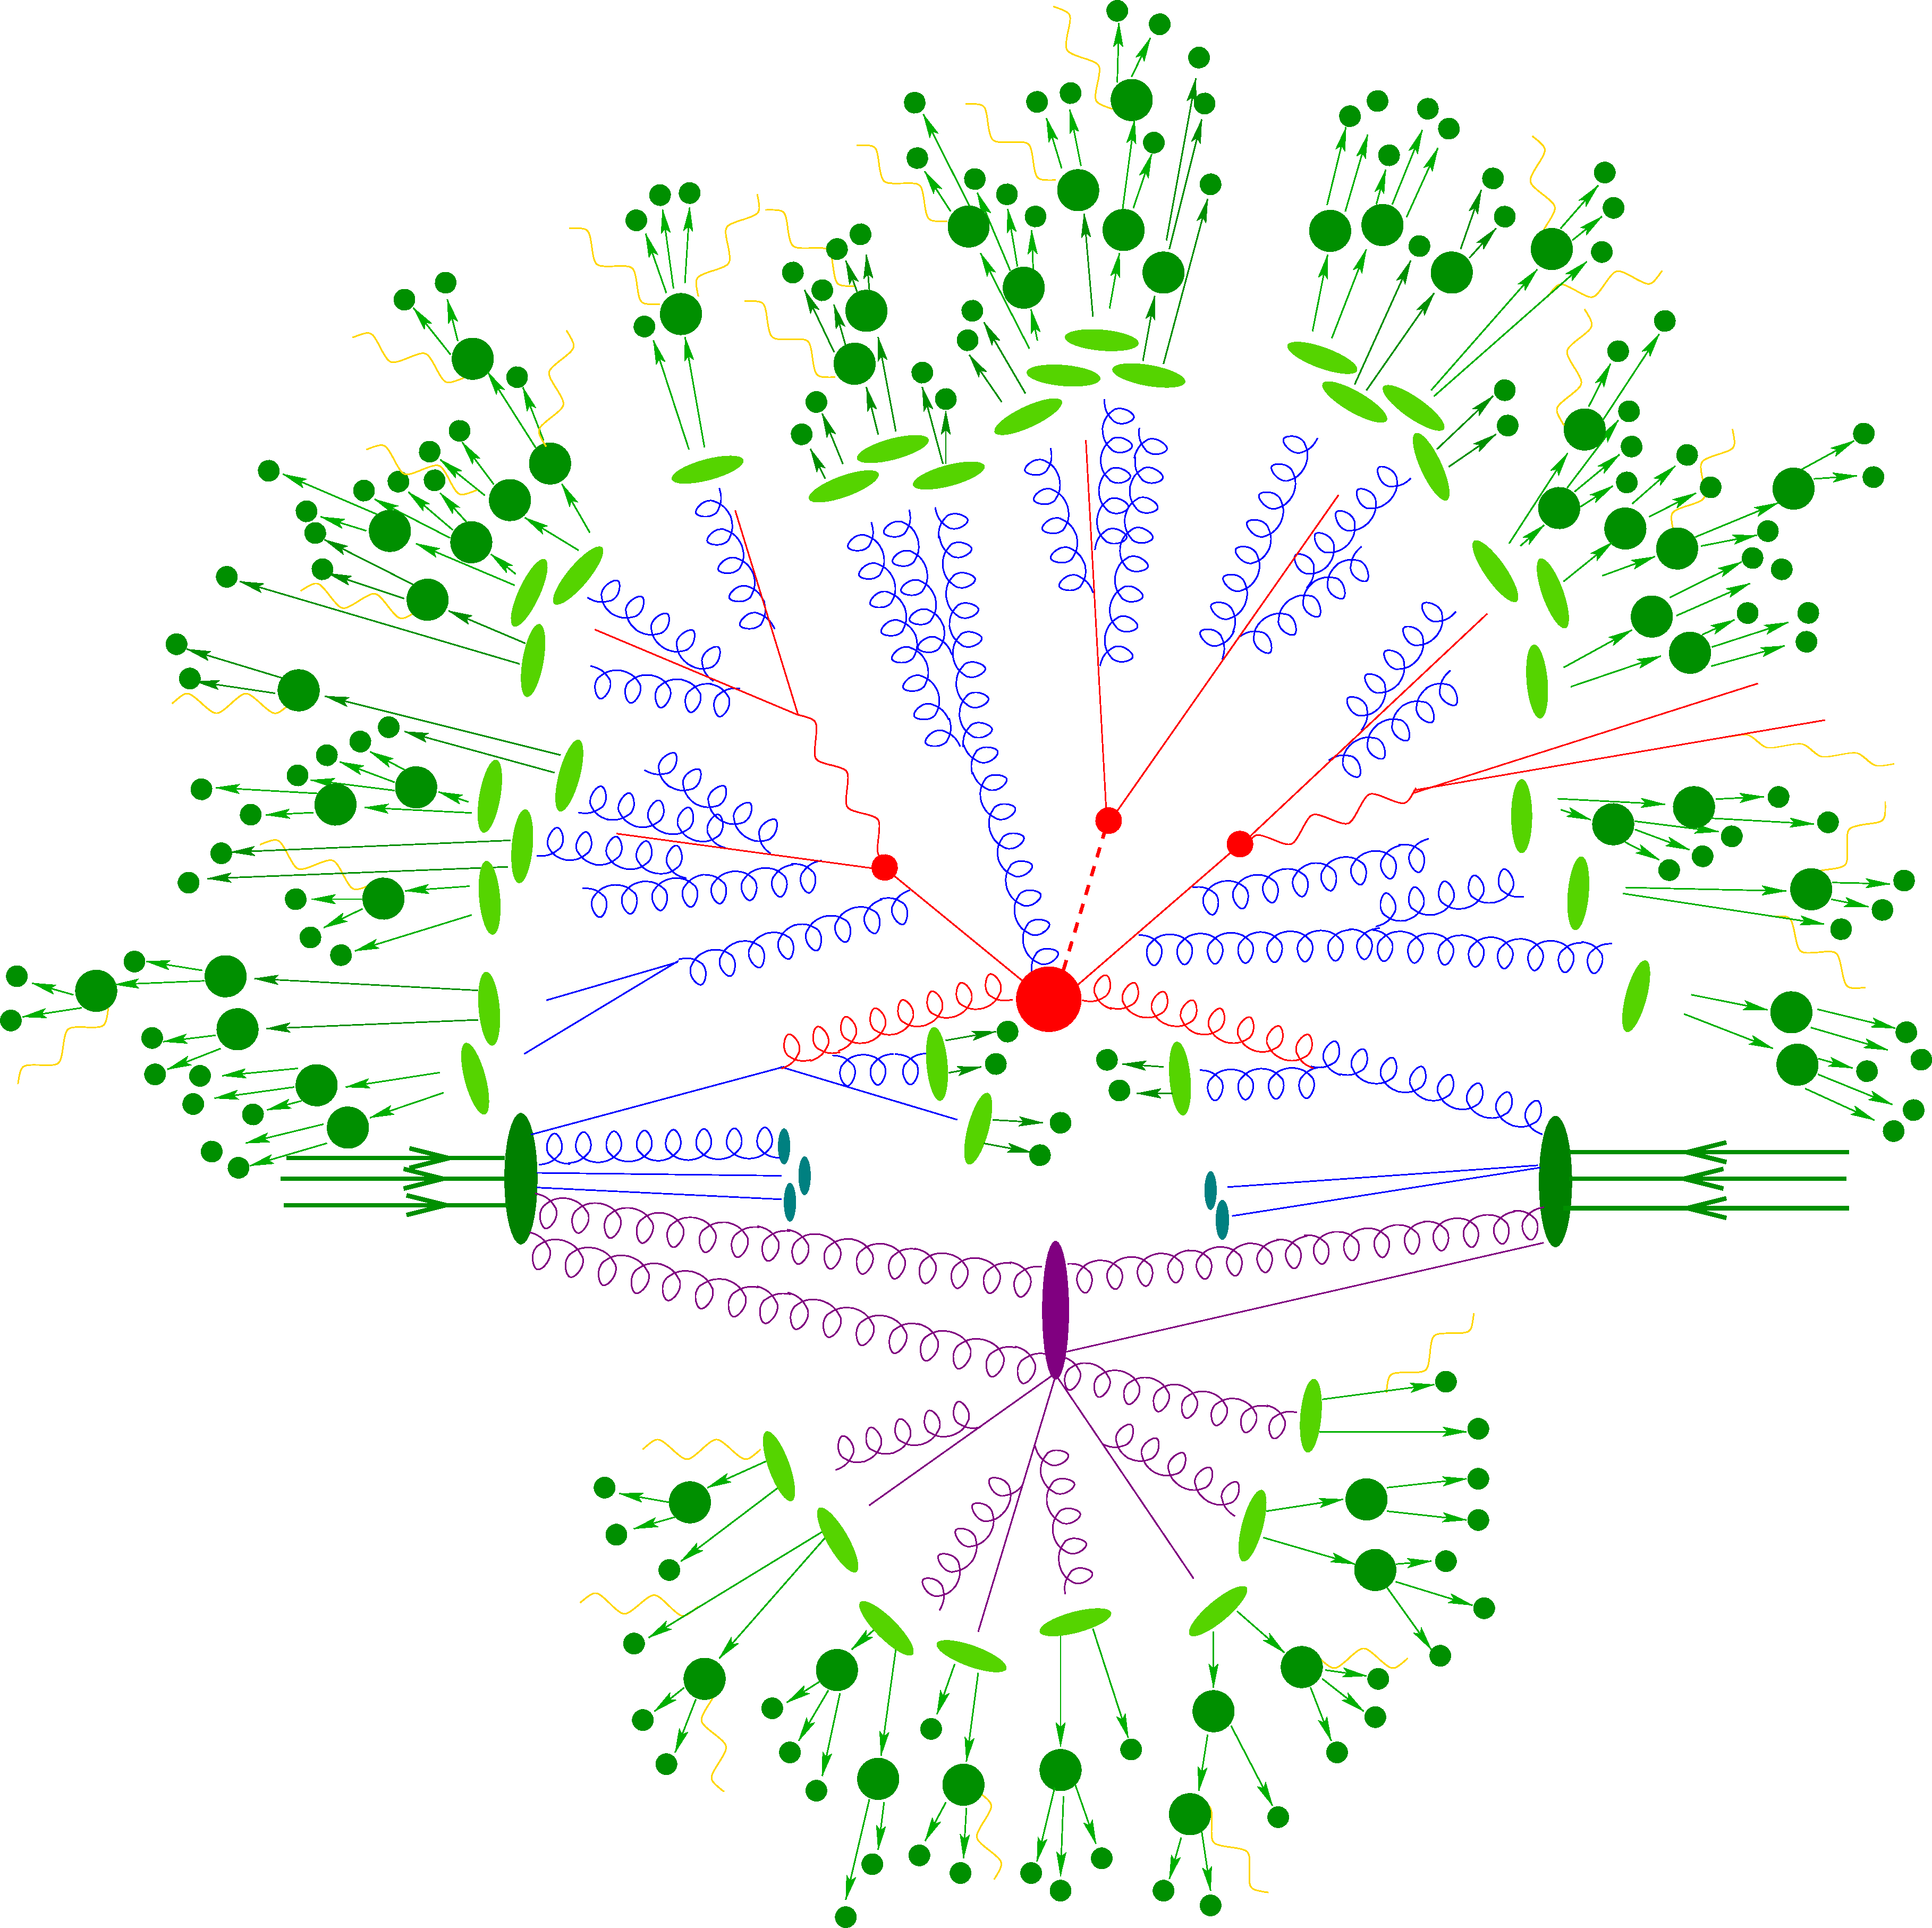
\includegraphics[width=0.6\textwidth]{figures/event_svg-tex.pdf}
  \caption{Schematic representation of the Monte Carlo event generation process in particle
           physics. Colouring of vertices and particles indicates the event generation stage:
           hard scattering process (big red blob), QCD radiation (blue), hadronisation (light
           green), showering (dark green), and a secondary vertex (purple).
           Taken from reference~\cite{sherpa_1}.}
  \label{fig:mc_stages}
\end{figure}
Building on the QCD processes introduced in \cref{sec:strong_interaction}, predictions at the \lhc are obtained almost exclusively via Monte Carlo (MC) simulations, in which event samples are generated by randomly sampling from the underlying probability distributions. The complex mathematical structure of the Standard Model, combined with the wide range of energy scales involved in collider processes, renders purely analytical predictions rarely feasible.

\paragraph{Hard scattering}
Events are simulated using a cascade of programs, each responsible for a distinct stage of the event. Matrix-element generators compute the hard-scattering amplitude for a given process and sample the kinematic phase space according to the differential cross-section, yielding the partonic final state of the hard interaction; events at this stage are referred to as
\textit{parton-level}.

\paragraph{Parton shower and hadronisation}
The parton-level events are subsequently passed through parton-shower and hadronisation algorithms, as outlined in \cref{sec:strong_interaction}, which evolve the hard-scatter partons into colour-neutral hadronic final states. A schematic description of the full event generation chain
is given in \cref{fig:mc_stages}.

\paragraph{Detector simulation}
Finally, detector simulation programs model the interactions of stable particles with the detector material, producing realistic detector responses. This includes simulating energy deposits in calorimeters, hits in tracking detectors, and other relevant signals. For many applications, a simplified fast simulation is sufficient, involving smearing of particle momenta and energies to match the detector resolution, applying efficiency corrections, and accounting for pile-up---the contribution from additional inelastic $pp$ interactions occurring within the same bunch crossing.


\section{Top-Quark Physics}
\label{sec:top-quark}
\begin{figure}[ht]
  \centering

  \begin{subfigure}[c]{0.3\textwidth}
    \centering
    \includegraphics[width=\textwidth]{figures/feynman-diagrams/ttbar_production_gg_t_channel.pdf}
    \caption{}
    \label{fig:top_production_gg_t_channel}
  \end{subfigure}
  \hfill
  \begin{subfigure}[c]{0.3\textwidth}
    \centering
    \includegraphics[width=\textwidth]{figures/feynman-diagrams/ttbar_production_gg_s_channel.pdf}
    \caption{}
    \label{fig:top_production_gg_s_channel}
  \end{subfigure}
  \hfill
  \begin{subfigure}[c]{0.3\textwidth}
    \centering
    \includegraphics[width=\textwidth]{figures/feynman-diagrams/ttbar_production_gg_u_channel.pdf}
    \caption{}
    \label{fig:top_production_gg_u_channel}
  \end{subfigure}
  \begin{subfigure}[b]{0.3\textwidth}
    \centering
    \includegraphics[width=\textwidth]{figures/feynman-diagrams/ttbar_production_qq_s_channel.pdf}
    \caption{}
    \label{fig:top_production_qq_s_channel}
  \end{subfigure}

  \caption{Leading order Feynman diagrams for top-quark pair production in \subrefb{fig:top_production_qq_s_channel}
     \subrefb{fig:top_production_gg_t_channel}, \subrefb{fig:top_production_gg_s_channel} \& \subrefb{fig:top_production_gg_u_channel} gluon fusion (ggF) and \subrefb{fig:top_production_qq_s_channel} quark-antiquark annihilation.}

  \label{fig:top_production}

\end{figure}

The top quark is the heaviest known elementary particle. The prediction of its existence arose due to the already established CP-Violation in the kaon system, which required a third generation of quarks to be explained within the SM framework~\cite{kobayashi_maskawa}. Furthermore, the discovery of the bottom quark in 1977~\cite{bottom_discovery} implied the existence of its weak isospin partner, the top quark. The top quark was eventually discovered in 1995 by the \cdf and \dzero collaborations at the \tevatron collider~\cite{top_discovery_cdf,top_discovery_d0}.
Currently, the world average of the top-quark mass is measured to be~\cite{PDG2024}
\begin{equation}
  m_t = 172.56 \pm 0.31~\unit{\giga\electronvolt}.
\end{equation}
Along with the largest mass, the top quark also has the strongest Yukawa coupling to the Higgs boson, making it interesting for studies of the Higgs mechanism and electroweak symmetry breaking.
Due to its large mass, the top quark also has the shortest lifetime of all quarks, about $5 \times 10^{-25}~\unit{\second}$~\cite{PDG2024}, which is shorter than the typical hadronisation timescale of $3 \times 10^{-24}~\unit{\second}$~\cite{hadronization_time_2}. Therefore, the top is the only quark that decays before it hadronises, allowing for direct studies of its properties through its decay products.

Notably, the top quark also decays before its spin can decorrelate, preserving spin information in the angular distributions of its decay products~\cite{spin_decorrelation_time}. This unique feature enables precise measurements of spin correlations and polarisation of top quarks.
At hadron colliders like the \lhc, top quarks are predominantly produced in pairs via the strong interaction.
The leading order (LO) Feynman diagrams for top-quark pair production are shown in \cref{fig:top_production}.
At the \lhc, the dominant production mechanism is gluon fusion (ggF).
This is due to the high gluon density in the proton at the relevant Bjorken-$x$ values for top-quark production and the low antiquark-contributions at a $pp$-collider.
The CKM matrix element $V_{tb}$ is close to unity~\cite{PDG2024}, leading to a nearly exclusive decay of the top quark into a $W$ boson and a $b$ quark.
The $W$ can subsequently decay either leptonically into a charged lepton and a neutrino or hadronically into a pair of quarks, with branching ratios of about $\text{BR}(W\to\ell,\nu)\approx1/3$ and $\text{BR}(W\to q\bar{q})\approx2/3$, respectively~\cite{PDG2024}.
Based on these $W$ decay modes, top-quark pair events are categorised into three channels. In the \textbf{dileptonic channel}, both $W$ bosons decay leptonically ($W^+ \to \ell^+ \nu_\ell$,$W^- \to \ell^-\bar{\nu}_\ell$), resulting in two charged leptons, two neutrinos and two $b$ quarks in the final state. This channel has a branching ratio of approximately $1/9$. The \textbf{semileptonic channel} occurs when one $W$ boson decays leptonically and the other hadronically ($W \to q\bar{q}'$), yielding one charged lepton, one neutrino, and four quarks (including two $b$ quarks) in the final state. Finally, in the \textbf{all-hadronic channel}, both $W$ bosons decay hadronically, producing six quarks (including two $b$ quarks) in the final state, which suffers from large multijet background contamination in the busy environment of hadron colliders like the \lhc. Both hadronic decays have a similar branching ratio of $4/9$.


\subsection{Spin Correlations in Top-Quark Pairs}
\label{sec:ttbar_entanglement}
As elaborated upon before, the top quark decays before it can hadronise or its spin decorrelates. Therefore, the spin information of the top quark is directly transferred to its decay products. In top-quark pair production, the spins of the top and antitop quarks are correlated due to the production mechanism. Due to the chiral nature of the weak interaction, these spin correlations manifest in the angular distributions of the decay products, particularly the charged leptons in the dileptonic decay channel.

Recent studies at the \lhc began to explore the potential effects of quantum entanglement in top-quark pairs~\cite{atlas_entanglement}. Entanglement generally describes a quantum mechanical phenomenon where the quantum states of two or more particles become correlated in such a way that the state of one particle cannot be described independently of the state of the other(s), even when the particles are separated by large distances~\cite{schrödinger_entanglement}. This property is expressed as the system having a non-separable density matrix. While a general description of this phenomenon is beyond the scope of this thesis, entanglement can be tested using specific criteria. One such criterion is the \emph{Peres-Horodecki criterion}~\cite{peres_criterion,entanglement_two_qbits}, which states that if the partial transpose of the density matrix of a bipartite system has at least one negative eigenvalue, then the system is entangled. Considering the top-quark pair's spin as a bipartite system of two spin-$\tfrac{1}{2}$ particles (qubits), this criterion can be applied to test for entanglement in their spin states.

In reference~\cite{entanglement_top_quarks}, it was proposed to measure entanglement in top-quark pairs produced at the \lhc by analysing the angular distributions of their decay products, specifically the charged leptons in the dileptonic decay channel. The study showed that by measuring the opening angle between the two leptons, one can construct an observable sensitive to the entanglement of the top quarks' spin system. Due to the kinematics of top-quark pair production, the entanglement is expected to be more pronounced in certain regions of phase space; one such region is at low invariant mass of the top-quark pair system.

One particular region of interest is the so-called \emph{threshold region}, referring to the region in which the invariant of ht \ttbar-system is close to the production threshold of $m(t\bar{t})\sim 350~\GeV$, where the top-quarks are produced with low relative velocity. In this region, the top-quark pair system is produced as a spin singlet state in about $\sim 80\%$ of the cases, leading to a strong entanglement signature~\cite{toponium_2}. The \atlas and \cms collaboration recently reported the first experimental evidence of quantum correlations consistent with entangled spin quantum states in top-quark pairs~\cite{atlas_entanglement,cms_entanglement}. Measurements of this variable are particularly sensitive in the dilepton channel, because the lepton has the highest spin-analysing power~\cite{spin_analyzing_power,spin_analyzing_power_jets}. The spin-analysing power measures the extent to which the spin information of the parent is imprinted in the angular distributions of the decay products. Due to QCD effects, this is lower for light jets compared to leptons.

\subsection{Top-Quark Pair Quasi-Bound-State Effects}
\label{sec:ttbar_toponium}
\begin{figure}[ht]
  \centering
  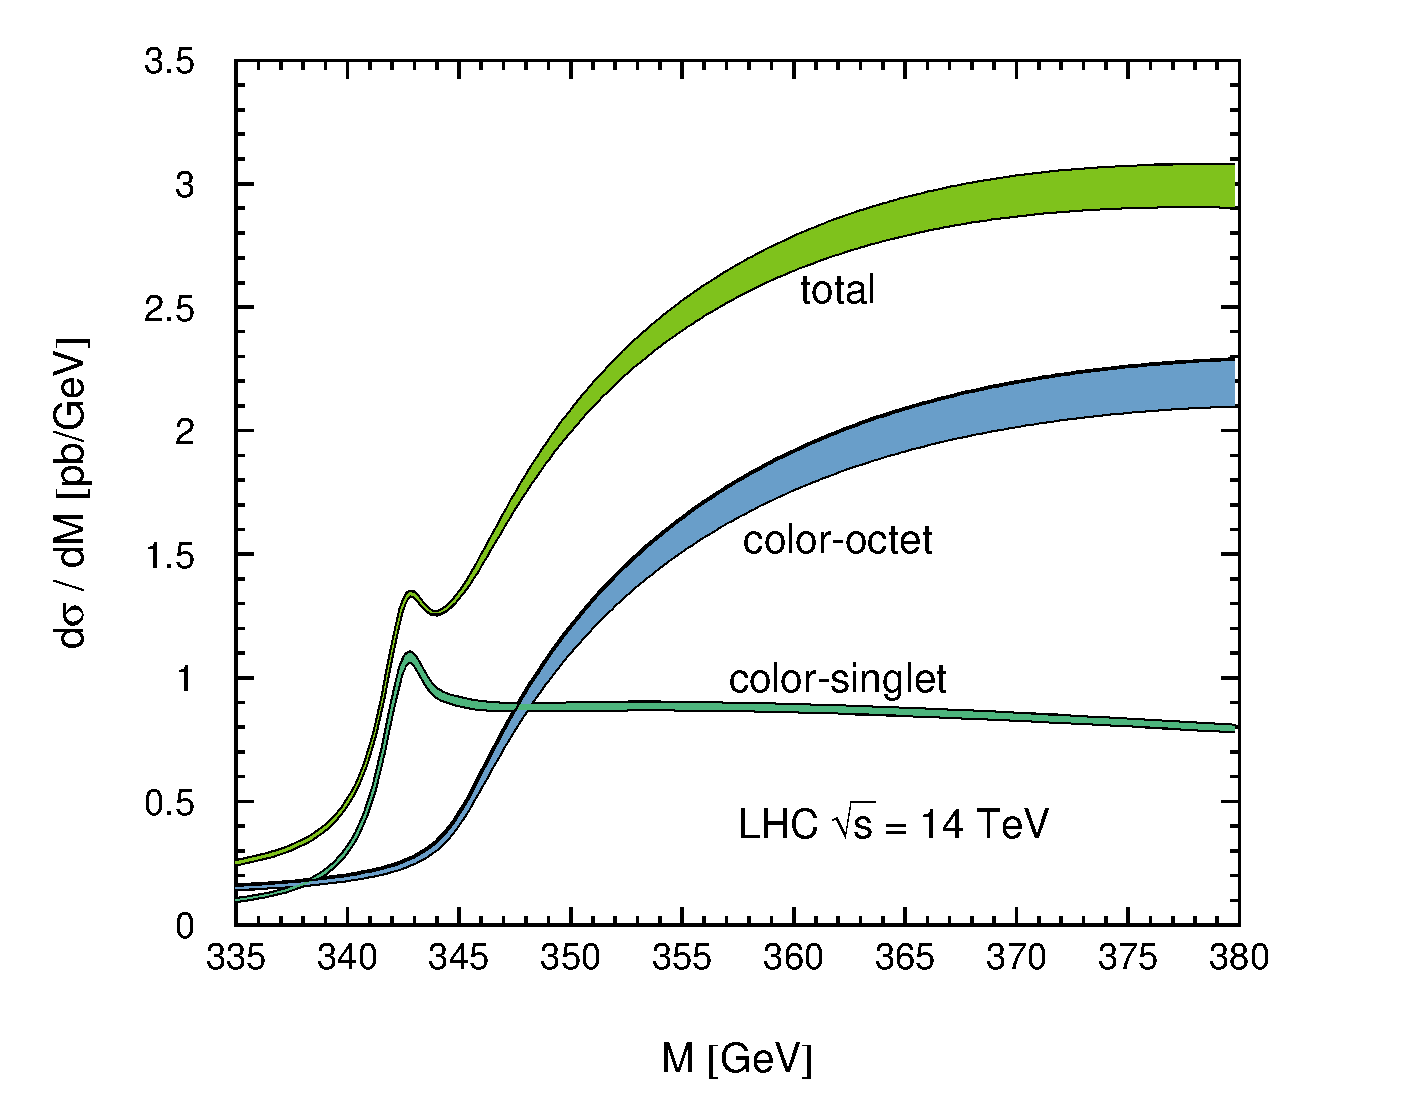
\includegraphics[width=.7\textwidth]{figures/toponium/xs2lhc14.pdf}
  \caption{Differential cross-section of top-quark pair production in     a colour-singlet or -octet state. The Figure is taken from     reference~\cite{toponium_2}, which provides further details on the   underlying modelling.}
  \label{fig:toponium_mttbar}
\end{figure}
Even though the top quark decays before it can hadronise, near the production threshold of top-quark pairs, the strong interaction between the top and antitop quarks can lead to the formation of transient bound states, coined as \textit{toponium}~\cite{toponium_1,toponium_2,toponium_3}. These bound state effects can influence the production cross-section and kinematic distributions of top-quark pairs near threshold. The \cms and \atlas collaborations have recently observed an excess in the invariant mass distribution of top-quark pairs near threshold, consistent with the presence of toponium-like bound state effects~\cite{CMS2025Pseudoscalar,atlas_toponium}. The modelling of these effects is based on non-relativistic QCD (NRQCD) calculations, which account for the strong interaction dynamics between the top and antitop quarks in the near-threshold region~\cite{NRQCD_toponium_1, NRQCD_toponium_2}. The leading contributions arise from the formation of colour-singlet $^1S_0$, which enhances the cross-section due to an attractive QCD potential. The differential cross-sections related to the different colour-states can be found in \cref{fig:toponium_mttbar}. A proper introduction to the physics behind this effect would exceed the scope of this thesis, which focuses on reconstruction techniques. Thus, for further reference, the reader is pointed to the aforementioned references \cite{NRQCD_toponium_1, NRQCD_toponium_2}.

Understanding and accurately modelling these bound-state effects is crucial for precision measurements of top-quark properties and for searches of new physics in top-quark pair production. One notable example is the measurement of quantum effects, where the strength of the observed entanglement properties is influenced by bound-state effects and by their impact on the spin structure of the top-quark pair system. The measurement of these effects relies on reconstructing the top-quark system at the production threshold and uses angular correlations among the top-quark's decay products, similar to studies of quantum effects.
\subsection{Dileptonic Decay Channel}
\label{sec:top_decay_modes}
\begin{figure}[ht]
  \centering
  \includegraphics[width=0.5\textwidth]{figures/feynman-diagrams/g_to_dilepton.pdf}
  \caption{Leading order Feynman diagram for top-quark pair   production via gluon fusion with dileptonic decay.}
  \label{fig:dilepton_ttbar_decay}
\end{figure}

While having the lowest branching ratio and thus the lowest event yields of all decay channels, the dilepton channel offers a particularly clean signature with reduced background contamination.
Furthermore, leptons can be reconstructed and identified with a high efficiency in a hadron-collider environment and carry charge information, which enables assignment to top or antitop quark, respectively.
This makes it very suited for precision measurements of top-quark properties. The presence of two neutrinos in the final state leads to missing transverse energy (\met) in the event, complicating the full reconstruction of the top quarks' kinematics. Advanced techniques, such as kinematic fitting and multivariate analyses, are often employed to address these challenges and extract maximum information from the dileptonic events.

\subsubsection{Kinematic Constraints}
\label{sec:kinematic_constraints}
Assuming both $W$ bosons and top quarks are on-shell, the following kinematic constraints can be applied to the dileptonic decay channel, 
\begin{alignat}{2}
  (\vec{p}_{\nu_1} + \vec{p}_{\nu_2})_{x} & = \met_x, &
  (\vec{p}_{\nu_1} + \vec{p}_{\nu_2})_{y} & = \met_y,  \label{eq:met}\\
  (p_{\ell_1} + p_{\nu_1})^2 & = m_W^2,  & (p_{\ell_2} + p_{\nu_2})^2 & = m_W^2, \label{eq:w_boson}    \\
  (p_{b_1} + p_{\ell_1} + p_{\nu_1})^2    & = m_t^2,\quad   & (p_{b_2} + p_{\ell_2} + p_{\nu_2})^2 & = m_t^2\,.\label{eq:top_quark_mass}
\end{alignat}
If one assumes the neutrinos to be massless, these six equations provide constraints on the six unknown components of the two neutrino momenta. Due to the algebraic nature of the constraints, multiple solutions can exist for a given event, leading to ambiguities in the reconstruction. Furthermore, the effects of detector resolution and off-shell particles can lead to the system of equations having no real-valued solution~\cite{sonnenschein_method, ellipse_method}. This motivates the development of more sophisticated reconstruction methods.

\subsection{Spin-Sensitive Angular Variables}
\label{sec:spin_sensitive_variables}
\begin{figure}[ht]
  \centering
  \begin{subfigure}[c]{0.49\textwidth}
    \centering
    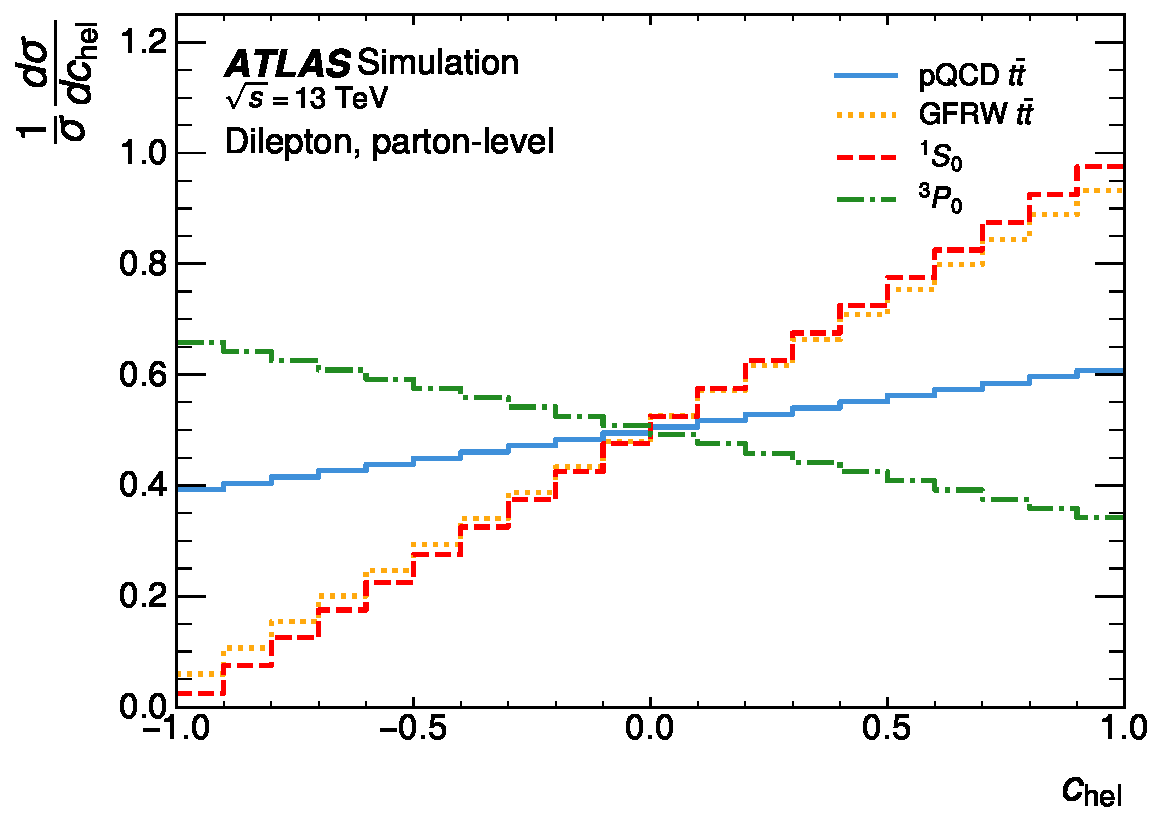
\includegraphics[width=\textwidth]{figures/c_hel_theory.pdf}
    \caption{\chel}
    \label{fig:c_hel_theory}
  \end{subfigure}
  \hfill
  \begin{subfigure}[c]{0.49\textwidth}
    \centering
    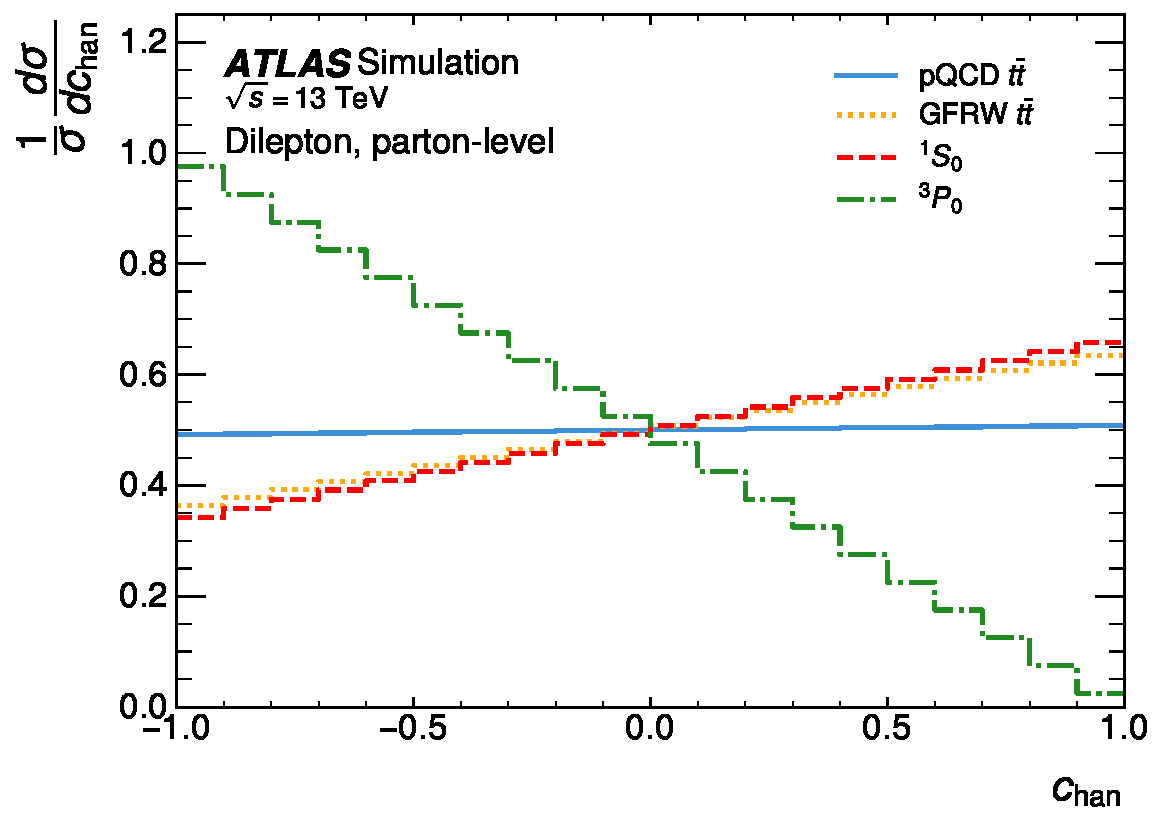
\includegraphics[width=\textwidth]{figures/c_han_theory.pdf}
    \caption{\chan}
    \label{fig:c_han_theory}
  \end{subfigure}
  \caption{Simulation of the distributions of  \chel and \chan for dileptonic decaying top-quark pairs produced near threshold. Distributions are shown for different spin states, as well as calculations using perturbative QCD (pQCD) or a modelling of the quasi-bound-state effects using a Green's Function Reweighting (GFRW)~\cite{NRQCD_toponium_2}. The distributions are normalised to unity and computed at parton level. The Figures are taken from   reference~\cite{atlas_toponium}.}
  \label{fig:spin_sensitive_theory}
\end{figure}


To study spin correlations and entanglement in top-quark pairs, a spin-sensitive angular variable is used. To measure quasi-bound-state effects, an additional angular variable is employed. Both variables are defined using the charged leptons from the dileptonic decay of the top-quark pair.

To compute the variables, top quarks and leptons are first boosted to the rest frame of the \ttbar system.

Their momentum vectors are boosted once more into their respective parent top quarks' rest frame. The normalised vectors of these transformed momenta are labelled as $\hat \ell_{t}^+$ and $\hat \ell^-_{t}$. The inner product of these unit vectors then defines the variable \begin{equation}
  \label{eq:c_hel}
  c_{\text{hel}} = \hat \ell_{t}^+ \cdot \hat \ell_{t}^-\,.
\end{equation}
Analogously, one can define the variable \chan, where either of the lepton momenta components parallel to the parent top-quark momentum in the \ttbar rest frame is flipped before taking the inner product \cite{bernreuther_nlospin_2004,bernreuther_spin_observables}. This variable adds important context by enabling isolation of scalar states. The differential cross-section of the spin-states as a function of \chel or \chan are obtained from simulation and found in \cref{fig:spin_sensitive_theory}. The distributions clearly show the distinctive shapes of the different spin states. Further, a stark difference between the slope of the perturbative QCD computation and the modelling of the quasi-bound state can be found, referred to as pQCD \ttbar and GFRW \ttbar in the plots, respectively.
This highlights the variables' sensitivity to the spin structure of the \ttbar system.


\chapter{Experimental Setup}
\label{chap:experiment_setup}
\section{The LHC}
The Large Hadron Collider (\lhc) at \cern is a synchrotron designed to accelerate protons and lead nuclei. This work focuses on the proton-proton collisions during \LHCrunii. During \LHCrunii from 2015
to 2018, the \lhc operated at a centre of mass energy of $\sqrt{s}=13\,\unit{\tera\electronvolt}$ with an integrated luminosity of $\mathcal{L}_{\text{int}}\approx 140\,\unit{\femto\barn^{-1}}$~\cite{ATLAS:2019pzw}.

After completion of \LHCruniii in June 2026 and an operational pause, the \lhc will operate with increased luminosity as the High-Luminosity Large Hadron Collider (HL-\lhc). During this phase, it is planned to accumulate data with an integrated luminosity of around $\mathcal{L}_{\text{int}}=3\,\unit{\atto\barn^{-1}}$
\cite{Aberle:2749422}.

\section{The Detector}
The \atlas detector is a general-purpose particle detector at the \lhc at \cern. It can be roughly separated into three elements: the inner detector, the calorimeter, and the muon spectrometer~\cite{atlas_tdr}.
\subsection{The Coordinate System}
The interaction point marks the origin of the \atlas coordinate system. The $z$-axis is orientated along the beamline, the $x$-axis points towards the centre of the \lhc and the $y$-axis points upwards.

Using this convention, several kinematic variables are defined. One of which is the transverse momentum defined as \begin{align}
p_T=\sqrt{p_x^2+p_y^2}
\end{align}
Because of the \atlas detector's cylindrical shape and the cylindrical symmetry of the interactions, the azimuthal angle is used as an additional variable. The polar angle relative to the $z$-axis can be used to define the pseudorapidity, which can also be expressed in terms of the momentum \begin{align}
\eta=-\ln\left(\tan\left(\frac{\theta}{2}\right)\right)=\ln\left(\frac{|\vec   p|+p_z}{|\vec p|-p_z}\right),.
\end{align}
In the ultra-relativistic limit $m\ll |\vec p|$, the pseudorapidity is equal to the rapidity defined as \begin{align}
y=\frac{1}{2}\ln\left(\frac{E+p_z}{E-p_z}\right),.
\end{align}
These variables are convenient for use in the \atlas experiment because $p_T,\phi$, and differences of $\eta$ are invariant under Lorentz-boost along the $z$-axis.
\subsection{Inner Detector}
\begin{figure}[ht]
\centering
\includegraphics[width=1.0\textwidth]{figures/atlas-detector/IDbriefing_figure1.png}
\caption{Schematic cross-section of the inner detector of the   \atlas detector (\copyright\ \cern).}
\label{fig:inner_det}
\end{figure} \noindent The inner detector (ID) is the innermost part of the \atlas detector.
It is used for tracking charged particles, particle identification, and primary- and secondary-vertex determination~\cite{atlas_tdr}. The ID consists of three different sub-detectors. Their rough structure is depicted in \Cref{fig:inner_det}. The ID is enclosed by a solenoid magnet, which provides a $2\,\unit{\tesla}$ axial magnetic field inside the ID. The magnetic field is crucial to measure the momentum of a charged particle. The transverse momentum is measured as the curvature of the particle's track due to the Lorentz force.

The detector part closest to the beam pipe is the pixel detector. It consists of 1744 modules arranged in three barrel layers. Each module hosts 47232 silicon pixels with a size of $50\times 400\,\unit{\micro \metre^2}$. The pixels are semiconductor trackers used to detect the traversing of charged particles.

The following part of the detector is the semiconductor tracker (SCT). It consists of 4088 modules arranged in four layers to ensure four-position measurements of charged particles. Each module consists of four silicon sensors. The sensors offer a $17\,\unit{\micro \metre}$ resolution in-plane lateral and $580\,\unit{\micro \metre}$ in-plane longitudinal.

The outermost part of the inner detector is the transition radiation tracker (TRT). It consists of polyimide drift (straw) tubes with a $4\,\unit{\milli\metre}$ diameter that are arranged in a $528\,\unit{\milli\metre}$ thick cylindrical layer around the beam pipe. The straw tubes are interleaved with fibres for the readout.
The transition radiation tracker utilises the transition radiation emitted by charged particles traversing the interface between two media with different refractive indices. The TRT provides measurements of charged particles and electron identification.
\subsection{Calorimeter System}
\begin{figure}[ht]
\centering
\includegraphics[width=0.85\textwidth]{figures/atlas-detector/0803015_01.jpg}
\caption{Computer generated image of the \atlas calorimeter   (\copyright\ \cern).}
\label{fig:colorimeter}
\end{figure}\noindent The calorimeters are the detector layers following the inner detectors. Its structure is divided into the Electromagnetic calorimeter (ECal) and the hadronic calorimeter (HCal).
\subsubsection{Electromagnetic Calorimeter}
The ECal is used for the energy and position measurement of electrically charged particles and photons. It utilises bremsstrahlung and pair production to create a cascade of charged particles, which are measured. Apart from offering full azimuthal coverage, it is equipped with end caps along the beam pipe. The \atlas ECal is a sampling calorimeter using lead as the passive medium and liquid Argon as the active medium. The innermost part of the ECal is a presampler that detects whether the particle started showering before reaching the ECal.
\subsubsection{Hadronic Calorimeter}
The HCal measures the energy and position of baryons and mesons through strong interactions with the nuclei. In the range $|\eta|<1.7$, it is a sampling calorimeter with steel as the passive medium and scintillators as the active medium. For the end cap, liquid Argon is deployed as the active medium. The HCal operates on the same principle as the ECal but provides less precise measurements. In the range of $3.1<|\eta|<4.9$, ECal and HCal are substituted with the forward calorimeters (FCal), which are made up of three modules to fulfil the function of both calorimeters. In combination with the FCal, the calorimeters cover the full range $|\eta|<4.9$.

A computer-generated image of the structures of the various calorimeters used in the \atlas detector is shown in \Cref{fig:colorimeter}.
\subsection{Muon Spectrometer}
The muon spectrometer is the outermost part of the \atlas detector.
Its purpose is to detect charged particles exiting the calorimeters and measure their momentum in the range of $|\eta|<2.7$. A detector dedicated to the measurement of muons is necessary because their mass makes them minimal ionising particles in the energy range of the \lhc collisions. The energy loss due to bremsstrahlung is insufficient to produce the showers needed to measure their energy. The muons' transverse momenta can be measured in the ID. Like the inner detector, the muon spectrometer utilises a magnetic field to conduct a measurement of the particle's momentum.  In the muon spectrometer, however, a solenoid magnet is used to allow for the measurement of the muon's momentum along a different direction. Combining the measurements yields complete knowledge of the muons' four-momentum.
Furthermore, the high rates of electron and hadron stopping in the calorimeters enable high specificity in muon detection.

\subsection{Trigger System}
With a bunch spacing of $25\,\unit{\nano\second}$
\cite{ATLAS:2019pzw} collisions happen at a rate of $40\,\unit{\mega\hertz}$. Each collision involves hundreds of particles. To reduce the data to a feasible amount, triggers are employed to filter out less interesting events. Different layers of triggers operate either at the hardware or software level. The L1 hardware-level trigger serves as the first filter for events. It makes decisions in less than $2.5\,\unit{\micro\second}$. The subsequent L2 trigger is a software-level trigger that makes decisions in less than $200 ,\unit{\micro \second}$. Combined, the trigger system reduces the event rate from $40\,\unit{\mega\hertz}$ to $1000\,\unit{\hertz}$. The events from this stream are then stored at the \cern data centre.
\chapter{Machine Learning in Particle Physics}
\label{chap:machine-learning}
Since this work focuses on improving the event reconstruction of dileptonic \ttbar decays using machine learning techniques, this chapter aims to provide an overview over the fundamental concepts and methodologies employed in machine learning.

From a computational perspective, machine learning can be viewed as the optimisation of a function $f:\mathbb{R}^n \rightarrow \mathbb{R}^m$ that maps input data points $\mathbf{x} \in \mathbb{R}^n$ to output predictions $\mathbf{y} \in \mathbb{R}^m$. The function $f$ is parameterised by a set of learnable parameters $\theta$, which are adjusted during the training process to minimise a predefined \textit{loss function} $L(\mathbf{y}, f(\mathbf{x}; \theta))$. The loss function quantifies the discrepancy between the predicted outputs and the true target values, guiding the optimisation process.


\section{Supervised Learning}
Machine learning can be broadly categorised into supervised and unsupervised learning. In supervised learning, the model is trained on a labelled dataset, where each input data point is associated with a corresponding target output. The goal of the model is to learn a mapping from inputs to outputs, enabling it to make accurate predictions on unseen data.


\subsection{Monte Carlo Training Data}
\begin{figure}
    \centering
    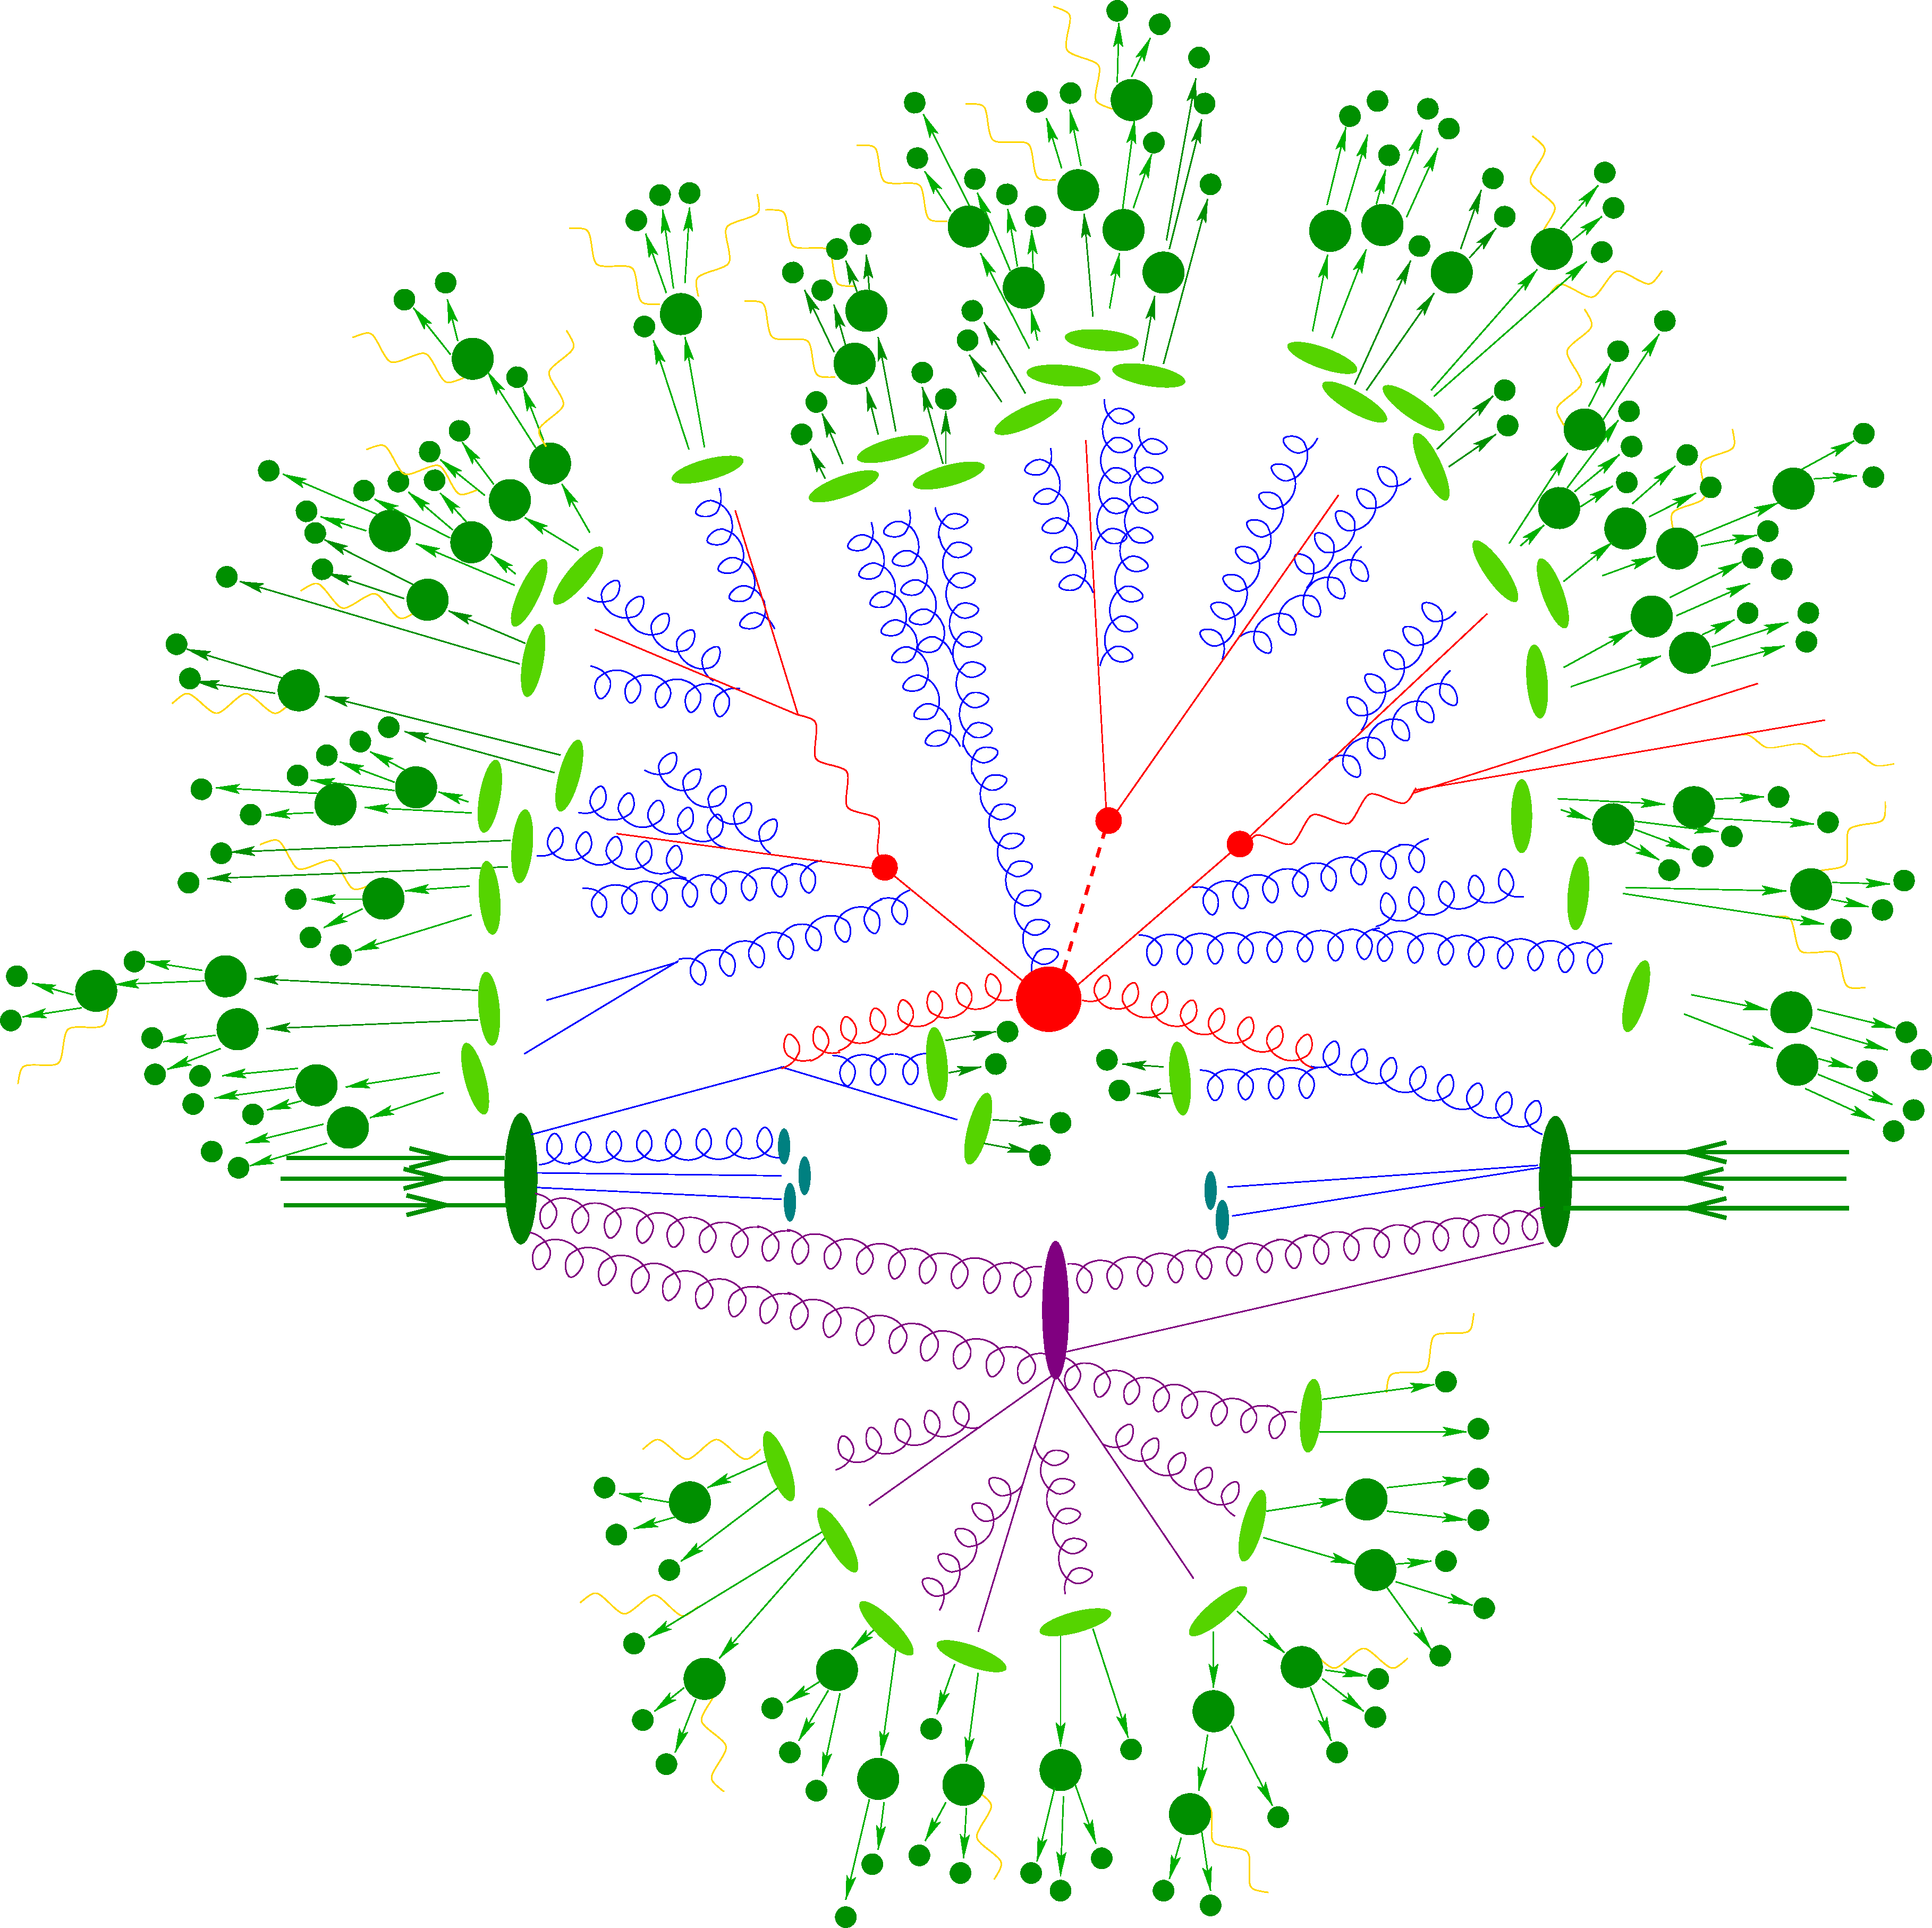
\includegraphics[width=0.6\textwidth]{figures/event_svg-tex.pdf}
    \caption{Schematic representation of the Monte Carlo event generation process in particle physics. Colouring of vertices and particles indicates the event generation stage: hard scattering process (big red blob), QCD radiation (blue), hadronisation (light green), showering (dark green), and a secondary vertex (purple). The Figure is taken from Reference~\cite{sherpa_1}.}
\end{figure}
\label{sec:mc_training_data}
Events are usually simulated using a cascade of different programs, each simulating a different state of the event. First the hard scattering process is simulated using matrix element generators. These programs calculate the probabilities of different particle interactions based on the underlying physics theories, such as the Standard Model. Using these probabilities, they generate events that represent the initial state of the particles after the collision. The possible kinematic phase space is sampled according to these probabilities, resulting in a set of particles with specific momenta and energies. This type of event variables is often referred to as \textit{parton-level}.

Next, the parton showering and hadronization processes are simulated. Parton showering models the emission of additional particles from the initial partons, while hadronization simulates the formation of hadrons from quarks and gluons. These processes are crucial for accurately modelling the final state particles observed in detectors.

Finally, detector simulation programs are used to simulate the interaction of particles with the detector material, producing realistic detector responses. This includes simulating the energy deposits in calorimeters, hits in tracking detectors, and other relevant signals.

While the actual detector response is simulated using complex detector simulation software, for many machine learning applications, a simplified representation of the detector response is sufficient. This can involve smearing the particle momenta and energies according to the detector resolution, applying efficiency corrections, and simulating the effects of pile-up.

This is because, for the reconstruction of the physics objects, such as jets, leptons, and missing transverse energy, highly sophisticated algorithms are used that already take into account the detector effects (Note that these algorithms may also be machine learning based). Therefore, the input features for machine learning models can often be derived directly from these reconstructed objects, rather than relying on the raw detector signals. The reconstructed object event variables are called \textit{reco-level}.

\subsection{Training}
During the training phase, the model is presented with a set of input features derived from the reco-level event variables, along with their corresponding target outputs, which are typically derived from the parton-level event variables. The model learns to map the input features to the target outputs by minimizing a loss function that quantifies the difference between the predicted and true values. Common loss functions include mean squared error for regression tasks and cross-entropy loss \cite{cross-entropy} for classification tasks.
The training process involves iteratively (each step is called \textit{epoch}) updating the model's parameters using an optimisation algorithm to minimise the loss function.

\subsection{Validation and Testing}
To evaluate the performance of the trained model, it is essential to validate and test it on independent datasets that were not used during training. This helps to assess the model's generalization capabilities and ensures that it can make accurate predictions on unseen data. A common practice is to split the available data into training, validation, and test sets. The validation set is used to tune hyperparameters and monitor the model's performance during training, while the test set is reserved for the final evaluation of the model's performance.

Since in particle physics, simulated data is often used for training and background modelling, one typically employs a k-folding strategy \cite{k-folding}, where the data is divided into k subsets. The model is trained k times, each time using a different subset as the validation set and the remaining subsets for training. This approach helps to use the available data more efficiently.

\section{Regression and Conditional Density Learning}
To highlight some important distinctions between different machine learning tasks, it is useful to briefly discuss regression and conditional density learning.
\subsection{Supervised Learning as Risk Minimisation}
In supervised learning, the goal is to learn a parametrised function $f_\theta$ that maps input data $\mathbf{x}$ to output predictions $\mathbf{y}$. This can be formalised as a risk minimisation problem, where the objective is to minimise the expected loss over the joint distribution of inputs and outputs. The expected risk can be expressed as:
\begin{equation}
    R(f) = \mathbb{E}_{\mathbf{x}, \mathbf{y}}[L(\mathbf{y}, f_\theta(\mathbf{x}))]
\end{equation}
where $L$ is the loss function that quantifies the discrepancy between the true output $\mathbf{y}$ and the predicted output $f_\theta(\mathbf{x})$. The goal of training is to find the parameters $\theta$ that minimise this expected risk, which is typically approximated using empirical risk minimisation on the training dataset.
\subsection{Regression}
In regression tasks, the output $\mathbf{y}$ is a continuous variable, and the model is trained to predict a specific value for each input $\mathbf{x}$. The loss function commonly used for regression is the mean squared error (MSE), which measures the average squared difference between the predicted values and the true values:
\begin{equation}
    L_{\text{MSE}}(\mathbf{y}, f(\mathbf{x})) = \frac{1}{N} \sum_{i=1}^{N} (y_i - f_\theta(\mathbf{x}_i))^2
\end{equation}
where $N$ is the number of samples in the dataset. The model learns to minimise this loss function. If the labels are not deterministic, meaning that there is inherent uncertainty in the target values, one can describe the labels using a conditional probability distribution $p(\mathbf{y}|\mathbf{x})$. In this case, minimising the MSE corresponds to learning the conditional mean of the distribution (see \Cref{chap:supplementary_computations_and_proofs} for a proof):
\begin{equation}
    f_\theta(\mathbf{x}) = \mathbb{E}[\mathbf{y}|\mathbf{x}] = \int \mathbf{y} p(\mathbf{y}|\mathbf{x}) d\mathbf{y}\,.
\end{equation}
Depending on the loss-function used, the model can learn different statistics of the conditional distribution. For example, using the mean absolute error (MAE) loss function would lead to learning the conditional median instead of the mean.

\subsection{Conditional Density Learning}
In contrast to regression, conditional density learning aims to learn the entire conditional probability distribution $p(\mathbf{y}|\mathbf{x})$ rather than just a point estimate. This is particularly useful when the target variable has inherent uncertainty or when multiple outcomes are possible for a given input. To quantify the difference between the true conditional distribution and the model's predicted distribution, the Kullback-Leibler (KL) divergence is often used as a loss function \cite{kl_divergence}
\begin{equation}
    L_{\text{KL}}(p, q) = \int p(\mathbf{y}|\mathbf{x}) \log \left( \frac{p(\mathbf{y}|\mathbf{x})}{q_\theta(\mathbf{y}|\mathbf{x})} \right) d\mathbf{y}
\end{equation}
where $p(\mathbf{y}|\mathbf{x})$ is the true conditional distribution and $q_\theta(\mathbf{y}|\mathbf{x})$ is the model's predicted distribution. Minimizing this loss function encourages the model to produce a predicted distribution that closely matches the true distribution, allowing for a more comprehensive understanding of the uncertainty and variability in the target variable. In practice, computing KL divergence can be challenging, since the true distribution might be unknown or difficult to estimate. In such cases, one relies on the data to provide an empirical estimate of the true distribution, and the loss function is approximated using samples from the dataset. It can be shown that minimizing the KL divergence is equivalent to maximizing the likelihood of the observed data under the model's predicted distribution, which is a common approach in training probabilistic models. For the case of a discrete target variable, this corresponds to minimising the cross-entropy loss, which is widely used in classification tasks \cite{cross-entropy}.

\section{Neural Networks}
\begin{figure}[ht]
    \centering
    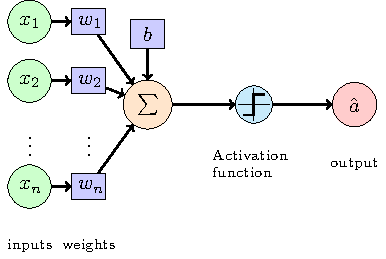
\includegraphics[width=0.6\textwidth]{figures/machine-learning/perceptron.pdf}
    \caption{Schematic of a single artificial neuron (perceptron). The neuron receives multiple input signals, each associated with a weight, and computes a weighted sum of these inputs, optionally a so-called bias is added. An activation function is then applied to this sum to produce the neuron's output.}
    \label{fig:perceptron}
\end{figure}
As elaborated before, machine learning models can be viewed as parameterised functions that map input data to output predictions. Neural networks are a class of machine learning models that are inspired by the structure and function of biological neural networks in the human brain. They consist of interconnected artificial neurons that process and transform the input data to produce the desired output.
The simplest unit of a neural network is the artificial neuron, also known as a perceptron \cite{perceptron}. A perceptron takes multiple input signals, each associated with a weight, and computes a weighted sum of these inputs. An activation function is then applied to this sum to produce the neuron's output. This structure is illustrated in \Cref{fig:perceptron}. The general structure of a perceptron is inspired by biological neurons. The activation function introduces non-linearity into the model, allowing it to learn complex patterns in the data. Common activation functions include the sigmoid function, hyperbolic tangent (tanh), and rectified linear unit (ReLU) \cite{relu}. For this work, the ReLU activation function is used, which is defined as $f(x) = \max(0, x)$, meaning that it outputs the input directly if it is positive, and zero otherwise. This activation function has been shown to be effective in training deep neural networks by mitigating the vanishing gradient problem \cite{relu}.


\subsection{Dense Neural Network}
\begin{figure}[ht]
    \centering
    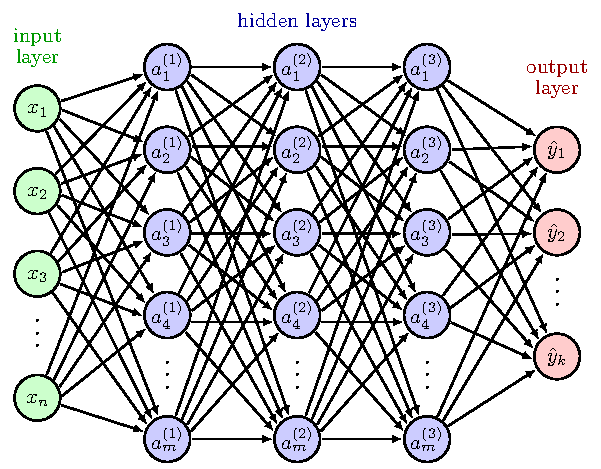
\includegraphics[width=0.5\textwidth]{figures/machine-learning/dnn.pdf}
    \caption{Schematic of a dense neural network with multiple layers. Each layer consists of multiple neurons, and each neuron in one layer is connected to every neuron in the subsequent layer.}
    \label{fig:dnn}
\end{figure}
A dense neural network (DNN), also known as a fully connected neural network \cite{backpropagation}, is a type of artificial neural network where each neuron in one layer is connected to every neuron in the subsequent layer. This architecture allows for the learning of complex relationships between input features and output targets. A schematic of a dense neural network is shown in \Cref{fig:dnn}.

A DNN consists of an input layer, one or more hidden layers, and an output layer. The input layer receives the input features, while the hidden layers perform a series of transformations on the data using the weights and biases associated with each neuron. The output layer produces the final predictions. Each layer applies an activation function to the weighted sum of inputs from the previous layer, enabling the network to learn non-linear mappings. The depth (number of layers) and width (number of neurons per layer) of the network can be adjusted.

\subsection{Transformer Networks}
\label{sec:transformer}
\begin{figure}[ht]
    \centering
    \begin{subfigure}[b]{0.3\textwidth}
        \centering
        \includegraphics[scale = 0.71]{figures/machine-learning/dpa.pdf}
        \caption{\centering Scaled \\ Dot-Product Attention}
        \label{fig:dpa}
    \end{subfigure}
    \begin{subfigure}[b]{0.35\textwidth}
        \centering
        \includegraphics[scale = 0.71]{figures/machine-learning/mha.pdf}
        \caption{Multi-Head Attention}
        \label{fig:mha}
    \end{subfigure}
    \begin{subfigure}[b]{0.3\textwidth}
        \centering
        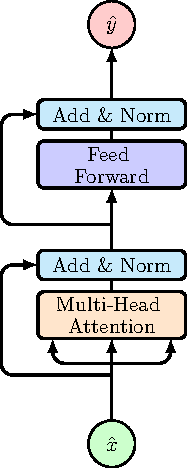
\includegraphics[scale = 0.71]{figures/machine-learning/transformer_layer.pdf}
        \caption{Transformer Layer}
        \label{fig:transformer_layer}
    \end{subfigure}
    \caption{Different components of the transformer architecture from smallest to largest unit: (a) Scaled Dot-Product Attention, (b) Multi-Head Attention, and (c) Transformer Layer.}
    \label{fig:attention}
\end{figure}
The transformer architecture deals with sequential data using an attention mechanism. This allows transformers to process information in parallel, making them efficient for training on large datasets. Additionally, transformer can capture long-range dependencies in the data very effectively, as they relate all elements of the input sequence to each other through attention mechanisms.

The core component of the transformer architecture is the attention mechanism, which allows the model to focus on different parts of the input sequence when making predictions. The most commonly used attention mechanism is the scaled dot-product attention \cite{attention_is_all_you_need}, illustrated in \Cref{fig:dpa}. In this mechanism, three vectors are computed for each input element: the query ($q$), key ($k$), and value ($v$) vectors. The attention scores are calculated by taking the dot product of the query and key vectors, scaling them by the square root of the dimension of the key vectors, and applying a softmax function to obtain attention weights. These weights are then used to compute a weighted sum of the value vectors, producing the output of the attention mechanism.
Multi-head attention, shown in \Cref{fig:mha}, extends the scaled dot-product attention by allowing the model to attend to different parts of the input sequence simultaneously. This is achieved by using multiple parallel attention heads, each with its own set of learned linear transformations for the query, key, and value vectors. The outputs of all attention heads are concatenated and linearly transformed to produce the final output.

The key, query and value vectors are typically obtained by applying learned linear transformations to the input embeddings. Depending on the type of relational information one wants to capture, one can choose to derive these vectors from different input sources. For example, in the \textit{self-attention mechanism}, all three vectors are derived from the same input sequence ($\hat q_t = \hat k_t=\hat v_t = \hat x_t$), allowing the model to relate different elements within the same sequence. In \textit{cross-attention}, the query vectors are derived from one sequence, while the key and value vectors are derived from another sequence ($\hat q_t = \hat x_{1,t}$, $\hat k_t=\hat v_t = \hat x_{2,t}$), enabling the model to relate information between two different sequences.
\paragraph{Symmetries}
In many applications, including particle physics, the input data exhibits certain symmetries that can be exploited to improve model performance.

The attention mechanism has inherent permutation equivariances, that can be exploited. Self-attention is permutation equivariant to the input sequence, meaning that permuting the input elements results in a corresponding permutation of the output elements. This property is particularly useful when dealing with sets or unordered data, where the order of the elements does not carry any inherent meaning. Cross-attention is permutation equivariant to permutations of the query inputs and separately to permutations of the key/value inputs. This allows the model to effectively relate information between two different sequences, regardless of their order.

\subsection{Training Neural Networks}
Training neural networks involves optimizing the model's parameters (weights and biases) to minimise the loss function. The number of parameters in a neural network can rise rapidly, especially in deep architectures, making the optimisation process computationally intensive. The most commonly used optimisation algorithm for training neural networks is stochastic gradient descent (SGD) \cite{sgd}, which iteratively updates the model's parameters based on the gradients of the loss function with respect to the parameters. Modern variants of SGD, such as Adam \cite{adam}, incorporate adaptive learning rates and momentum to improve convergence.
The backpropagation algorithm \cite{backpropagation} is used to efficiently compute the gradients of the loss function with respect to the model's parameters. It involves propagating the error signal backward through the network, allowing for the calculation of gradients at each layer. These gradients are then used by the optimisation algorithm to update the parameters. The algorithm relies on the chain rule and nested structure of the neural network to compute the gradients efficiently.
Regularization techniques, such as dropout \cite{dropout} and weight decay, are often employed during training to prevent overfitting and improve the model's generalization capabilities. Dropout randomly deactivates a fraction of the neurons during training, forcing the network to learn more robust features. Weight decay \cite{adamW} adds a penalty term to the loss function based on the magnitude of the weights, discouraging overly complex models and promoting generalization.
\chapter{Analysis and Reconstruction of Dileptonic Top-Quark Pair Events}
\label{chap:reconstruction-methods}
\section{Data and Simulation}
\label{sec:data-and-simulation}

This section describes the data and simulation samples used in this analysis. At the current stage of this thesis, only simulation samples have been studied; the data samples will be described in the final version. The simulated samples are produced using Monte Carlo (MC) event generators as described in \Cref{sec:mc_training_data}.

While a complete analysis requires detailed investigation of background processes contributing to the signal regions, this thesis focuses on developing and evaluating reconstruction methods. Therefore, only the signal process of \ttbar production with dileptonic decays is described here. The background processes and their simulation will be discussed in the final thesis.

\subsection{Simulation of Dileptonic Top-Quark Pair Events}
\label{sec:nominal_ttbar}
The signal process of \ttbar production with dileptonic decays is simulated using \powheg~\cite{powheg} at next-to-leading order (NLO) in perturbative quantum chromodynamics (QCD). The \powheg generator is interfaced with \pythia~\cite{pythia} for parton showering, hadronization, and underlying event modelling.

To link the reco-level particles to the parton-level objects, a parton matching is performed. The parton-level objects are defined as the top quarks and their decay products after final state radiation before hadronization. The matching is done by iteratively associating reconstructed jets to partons based on angular distance criteria. The decay products of the top quarks are matched within a cone of $\Delta R \leq 0.3$ and $\Delta R\leq 0.1$ for jets and leptons ($e$,$\mu$) respectively. If multiple reconstructed objects are found within this cone, the one with the smallest $\Delta R$ is chosen.

\subsection{Simulation of Non-Relativistic Quasi-Bound State Resonance}



\subsection{Object Definition}
\label{sec:object-definition}
The reconstruction of physics objects—electrons, muons, jets, and missing transverse energy (\met)—is performed using the standard \atlas reconstruction algorithms~\cite{atlas_tdr}.

\paragraph{Electrons} are required to have transverse momentum \pt $> 5~\unit{\giga\electronvolt}$ and pseudorapidity $|\eta| < 2.47$, excluding the transition region between the barrel and endcap calorimeters ($1.37 < |\eta| < 1.52$). Electrons must satisfy the Tight identification criteria and be isolated from other activity in the detector.

\paragraph{Muons} are reconstructed using information from both the inner detector and the muon spectrometer. They are required to have \pt $> 5~\unit{\giga\electronvolt}$ and $|\eta| < 2.5$. Muons must satisfy the Tight identification criteria and be isolated.

\paragraph{Jets} are reconstructed using the anti-$k_t$ algorithm \cite{anti_k_t_jet_2} with a radius parameter of $R = 0.4$. They are required to have \pt $> 25~\unit{\giga\electronvolt}$ and $|\eta| < 2.5$. $b$-tagging is performed using the GN2 algorithm~\cite{gn2_btagger} to identify jets originating from $b$-quarks.

\paragraph{Missing Transverse Energy} (\met) is calculated from the negative vector sum of the transverse momenta of all reconstructed objects in the event, including a soft term to account for energy not associated with reconstructed objects.

\subsection{Event Selection}
\label{sec:event-selection}
Events are selected to contain exactly two oppositely charged leptons (electrons or muons). One of the leptons must have \pt $> 25~\unit{\giga\electronvolt}$, while the other must have \pt $> 5~\unit{\giga\electronvolt}$. At least two jets are required, with at least one being $b$-tagged at the $77\%$ working point (WP). Additional selection criteria are applied to suppress background contributions, which will be detailed in the final thesis.

For the training and evaluation of the reconstruction methods, only events that pass the selection criteria and have a successful parton matching are considered. Fully parton-matched events, make up about $60\%$ of the whole sample. Events with jets or leptons of the \ttbar-process end up outside the detector acceptance are typically the main cause for an event being unmatchable. Thus, training with only parton-matched events might introduce a bias with respect to certain event topologies, if they are disfavoured to have a parton-matching.


\section{Reconstruction of Top-Quark Pairs}
\label{sec:reconstruction-methods}
Reconstructing the kinematics of dileptonic \ttbar events requires an assignment of reconstructed objects to the parton-level decay products. This section describes the different reconstruction methods developed and evaluated in this thesis.

While the leptons are directly identified from the reconstructed objects, the assignment of jets to the $b$-quarks from the top quark decays is ambiguous due to the presence of multiple jets in the event. Additionally, the two neutrinos from the $W$ boson decays are not directly detected, leading to missing information in the event reconstruction.
Based on this, the reconstruction breaks down into two main tasks:
\paragraph{Jet Assignment} Assigning the reconstructed jets to the $b$-quarks from the top quark decays.
\paragraph{Neutrino Regression} Estimating the momenta of the two neutrinos using the measured \met and other event kinematics.

\subsection{B-Tagging}
\label{sec:b_tagging}
The identification of $b$-jets is crucial for the reconstruction of \ttbar events. Due to the long lifetime of $b$-hadrons, they travel a measurable distance from the primary vertex before decaying, leading to displaced vertices and tracks with large impact parameters. The GN2 algorithm \cite{gn2_btagger} is used for $b$-tagging in this analysis, which combines various discriminating variables using a deep (graph) neural network to achieve high efficiency and purity in identifying $b$-jets. The performance of the $b$-tagging algorithm is characterised by its efficiency (the probability of correctly identifying a $b$-jet) and its misidentification rate (the probability of incorrectly tagging a non-$b$-jet as a $b$-jet).


\subsection{Jet Assignment Methods}
\label{sec:jet_assignment}
This thesis explores several methods for jet assignment, ranging from traditional algorithms to machine learning approaches. While the leptons can be assigned to the $W$ bosons based on their charge, the assignment of jets to the $b$-quarks is not straightforward due to the presence of multiple jets in the event. All the methods presented here, utilise kinematic relationships to make an assignment which jet and lepton stem from the same top quark decay.
From recent publications e.g. \cite{ATLAS2024Entanglement}, two conventional methods have been implemented as baselines:

\paragraph{Jet-Selection}
Both methods start by selecting the two $b$-jet candidates in the event based on the $b$-tagging at the $77\%$ WP. If more than two $b$-tagged jets are present, the two with the highest \pt are chosen. If only one $b$-tagged jet is found, the non-tagged jet with the highest $b$-tagging score is selected as the second candidate.
\begin{figure}[H]
    \centering
    \begin{minipage}[t]{0.48\textwidth}
        \textbf{$\chi^2$-Method}\\[0.5em]
        For both possible assignments of the two $b$-jet candidates to the parton-level $b$-quarks, the invariant masses of the reconstructed top quarks are computed,
        \begin{equation}
            \label{eq:chi_square}
            \chi^2 = (m_{b_1,{\nu},\ell^+} - m_{t})^2+(m_{b_2,\bar{\nu},\ell^-} - m_{t})^2
        \end{equation}
        where $m_t = 172.5~\unit{\giga\electronvolt}$ is the top quark mass. The assignment with the smaller $\chi^2$ value is chosen.
    \end{minipage}
    \hfill
    \begin{minipage}[t]{0.48\textwidth}
        \textbf{$\Delta R$-Method}\\[0.5em]
        This method assigns the $b$-jet candidates based on their angular distance to the leptons.
        \begin{equation}
            \Delta R = \sqrt{(\Delta\phi)^2 + (\Delta\eta)^2}
        \end{equation}
        The jet-lepton-pair with the smaller $\Delta R$ value is assigned to each other. The remaining jet is assigned to the other lepton.
    \end{minipage}
\end{figure}
Note, that the $\chi^2$-Method relies on the reconstructed neutrino momenta to compute the invariant masses of the top quarks. Therefore, it is inherently linked to the neutrino regression method used. In contrast, the $\Delta R$-Method is independent of the neutrino momenta.
For the analysis here, the regression from $\nu^2$-Flows was found to deliver a much better performance for the assignment. Thus, ultimately, the $\chi^2$-Method was used in conjunction with the prediction of $\nu^2$-Flows instead of the $\nu$-Weighter to provide a reasonable baseline.

Empiric evidence for the validity of both can be found in \Cref{fig:jet_lepton_pairing}, which shows the distributions of the reconstructed invariant mass of the top quark and the $\Delta R$ between the jet and lepton for correct and incorrect jet-lepton pairs. The correct pairs show a clear peak around the top quark mass in the invariant mass distribution and a smaller $\Delta R$ compared to incorrect pairs, which supports the use of these variables for jet assignment.

The $\Delta R$-Method was used in previous \atlas analyses \cite{ATLAS2024Entanglement} for events, that failed the kinematic reconstruction required for the $\chi^2$-Method. However, in this thesis, both methods are evaluated on the full dataset for comparison. 

\begin{figure}
    \centering
    \begin{subfigure}{0.49\textwidth}
        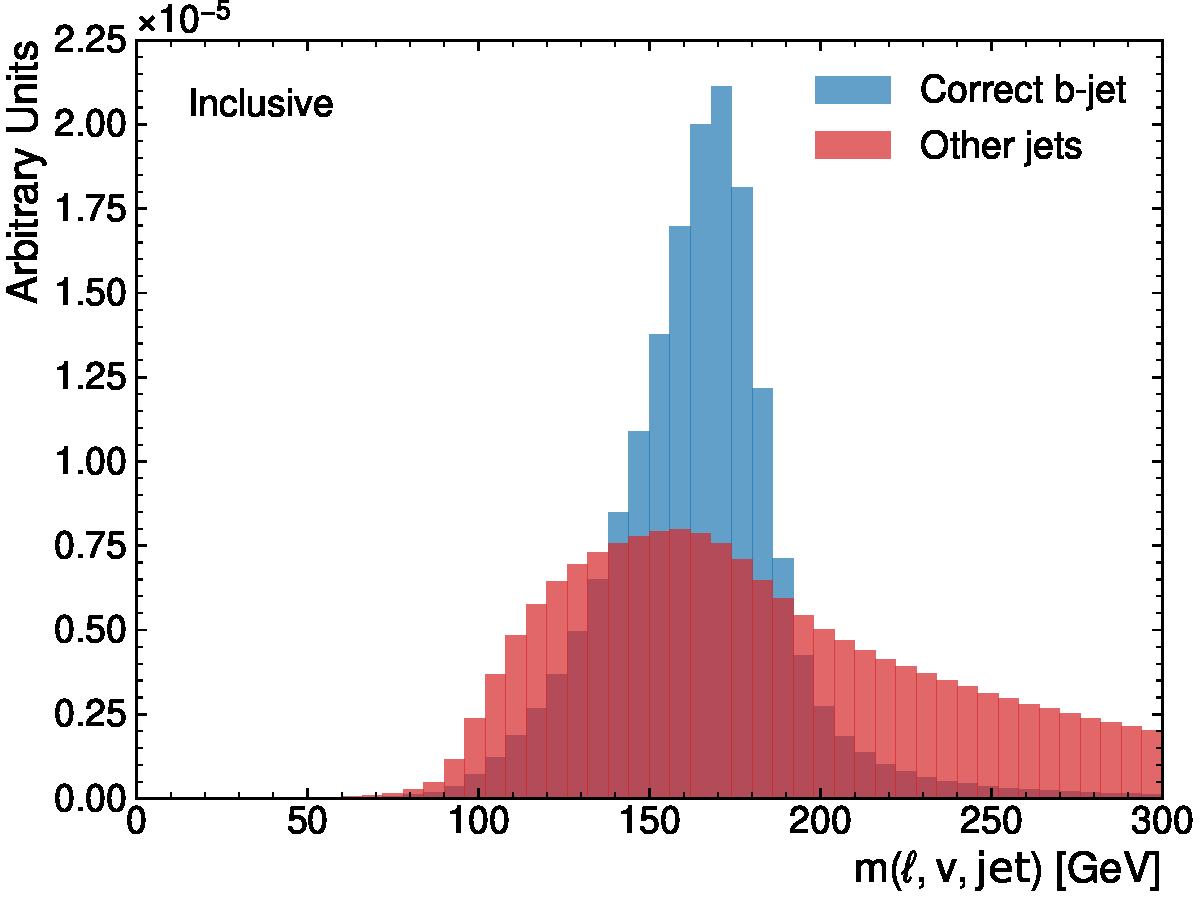
\includegraphics[width=\textwidth]{plots/feature_plots/relational_jet_lepton_full_inv_mass_distribution.pdf}
        \caption{$\chi^2$-Method}
        \label{subfig:chi_square_method}
    \end{subfigure}
    \begin{subfigure}{0.49\textwidth}
        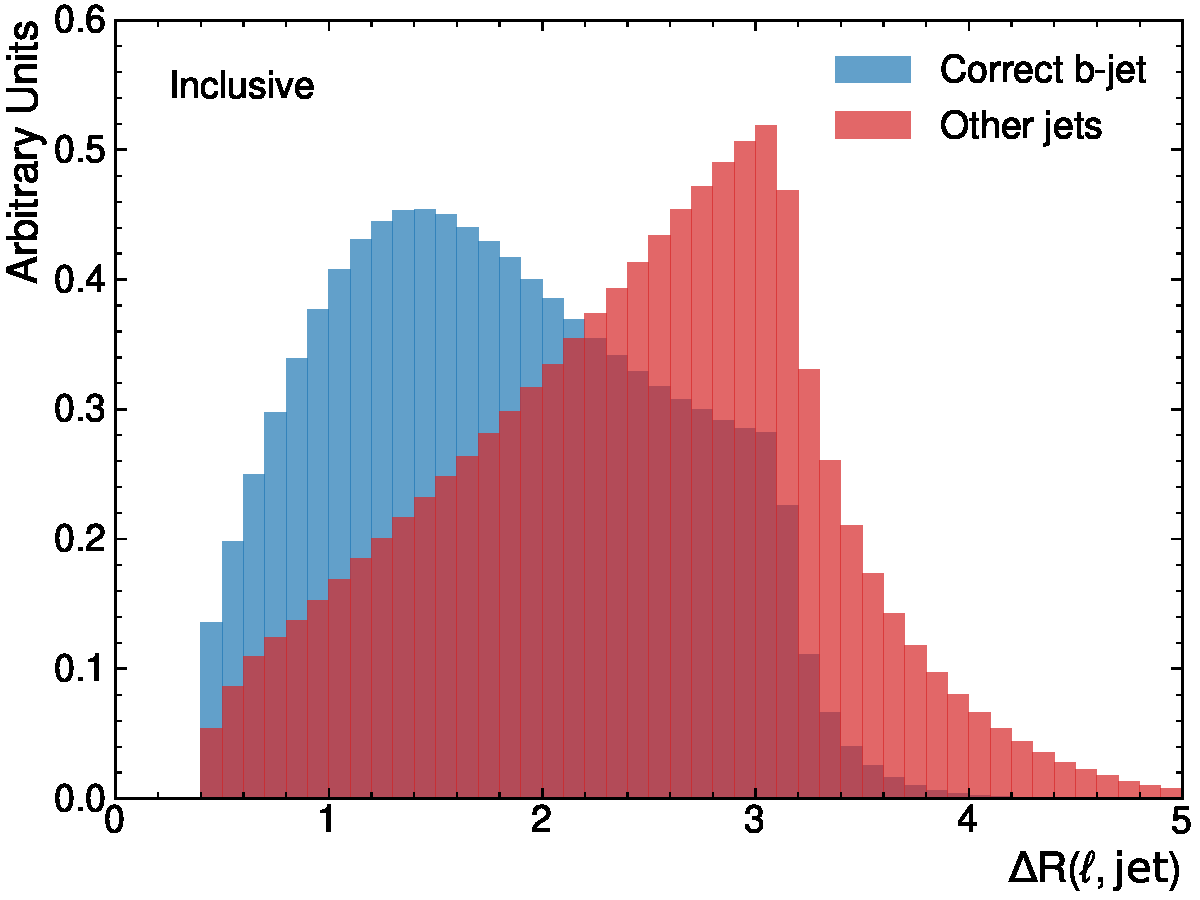
\includegraphics[width=\textwidth]{plots/feature_plots/relational_jet_lepton_deltaR_distribution.pdf}
        \caption{$\Delta R$-Method}
        \label{subfig:delta_R_method}
    \end{subfigure}
    \caption{Distributions for pairing up correct and incorrect jet-lepton pairs for the reconstructed invariant mass of the top quark (a) and the $\Delta R$ between the jet and lepton (b). The correct pairs are shown in blue, while the incorrect pairs are shown in red. The distributions are normalised to unit area. Note, that the reconstructed invariant mass for the $\chi^2$-Method includes the neutrino prediction from $\nu^2$-Flows.}
    \label{fig:jet_lepton_pairing}
\end{figure}

\subsection{Neutrino Regression Methods}
\label{sec:neutrino_regression}
Due to the limited availability of kinematic reconstruction methods in the \atlas software framework, two methods for neutrino regression are implemented and evaluated in this thesis. For completeness, the Ellipse-method, which has been used in previous \atlas analyses is described as well, but they have not been implemented or evaluated in this thesis.


\subsubsection{Ellipse-Method}
The ellipse method \cite{ellipse_method} is a kinematic reconstruction technique that exploits the constraints of the event to solve for the neutrino momenta. The method uses the measured \met and the momenta of the leptons and jets to construct a system of equations based on the invariant mass constraints of the $W$ bosons and top quarks. By solving this system of equations, one can obtain possible solutions for the neutrino momenta. The method typically yields multiple solutions, and additional criteria are used to select the most likely solution based on the event kinematics. In previous \atlas analyses, the solution yielding the lowest $m(t\bar{t})$ was chosen as the reconstructed neutrino momenta.

\subsubsection{Neutrino-Weighter}
The Neutrino-Weighter ($\nu$-Weighter), first described in \cite{neutrino_weighting_method}, is a method that assigns weights to different possible neutrino momentum configurations based on how well they satisfy the kinematic constraints of the event. The method uses the measured \met and the momenta of the leptons and jets to compute a weight for each possible neutrino momentum configuration. For each configuration, a weight is computed based on how well the reconstructed event kinematics match the expected kinematics of a \ttbar event - this includes constraints such as the invariant mass of the $W$ bosons and top quarks. The configuration with the highest weight is then selected as the reconstructed neutrino momenta. This method is computationally intensive, as it requires scanning over numerous possible neutrino momentum configurations. The computation of the reconstructed masses for the tops and W-bosons requires identification of the jets with a lepton. In principle this might be done by a sophisticated method such as the ones presented here.
However, the implementation used here, selected the jets based on b-tagging at $85\%$ working-point, and leading $p_T$ in case, the number of b-tagged jets deviates from two. While this still leaves a two-fold degeneracy for the assignment, both of the scenarios were evaluated, weighted and considered for the maximisation of the likelihood.

\subsubsection{$\nu^2$-Flows}
The method $\nu^2$-Flows \cite{nu_square_flows} uses normalizing flows to model the conditional probability distribution of the neutrino momenta given the observed event kinematics. The model is trained on simulated dileptonic \ttbar events, where the true neutrino momenta are known from the parton-level information. The trained model can then be used to sample possible neutrino momenta for new events, allowing for a probabilistic reconstruction of the event kinematics. For each event, multiple samples of neutrino momenta are drawn from the model, and the one with the highest probability density is selected as the reconstructed neutrino momenta.
A detailed outline of the $\nu^2$-Flows method and its implementation can be found in Reference~\cite{nu_square_flows}. For this thesis, this method serves to establish a baseline for neutrino regression to evaluate the impact of improved jet assignment methods. Note, however, that this method has not been used in \atlas analyses yet. However, due to matters of software compatibility, it was one of the only viable options at this stage of the thesis.
Since $\nu^2$-Flows processes the full event information to make a prediction for the neutrino momenta, it does not require a jet-assignment. Therefore, it can be used in conjunction with both the $\chi^2$-Method and the $\Delta R$-Method for jet assignment, allowing for a direct comparison of the impact of the jet assignment on the overall reconstruction performance.
\chapter{Machine Learning Based Reconstruction}
\label{chap:ml-reconstruction}


In addition to the outline reconstruction methods described in \Cref{chap:reconstruction-methods}, this chapter focuses on the development of a machine learning-based reconstruction strategies for the dileptonic \ttbar channel. Machine learning-based reconstruction techniques have gained significant traction in recent years. One major example for this, is their use in flavour tagging algorithms \cite{flavour_tagging_review}. For this, machine learning models are trained to address both challenges of jet assignment and neutrino regression, by learning from simulated data to predict the correct jet-parton assignments and neutrino momenta.

For the high permutation complexity of jet assignments in all-hadronic channels, SPANet \cite{spanet} has demonstrated significant improvements over traditional methods. These architectures leverage attention mechanisms to improve the accuracy by leveraging the full event information and utilising permutation equivariant architectures to handle the combinatorial nature of the problem.
Based on these successes, this thesis explores the adaptation of similar architectures for the dileptonic \ttbar channel, which presents unique challenges due to the presence of two neutrinos and fewer jets.

On the other hand, for neutrino regression, $\nu^2$-Flows \cite{nu_square_flows} has shown promise in improving the reconstruction of neutrino momenta by modelling the underlying probability distributions of the neutrino kinematics.

This thesis investigates, how machine learning can be used to provide a full reconstruction pipeline for the dileptonic \ttbar channel, by combining jet assignment and neutrino regression.

\section{Jet-Assignment}
\label{sec:jet-assignment}

\subsection{Neural Network Architectures}
\label{sec:nn-architectures}


\subsection{Training Procedure}
\label{sec:training-procedure}

\subsection{Hyperparameter Optimisation}
\label{sec:hyperparameter-optimisation}

\section{Neutrino Regression}
\label{sec:neutrino-regression}


\chapter{Evaluation of the ML-Based Reconstruction}
\label{chap:performance-evaluation}
To evaluate the performance of the ML-based reconstruction method, several metrics and analyses are conducted. This chapter presents the results of these evaluations, focusing on the accuracy of particle assignments, the reconstruction of relevant physics variables, and the performance across different kinematic regions. For this evaluation, the ML-based methods are compared against the baseline reconstruction techniques. The comparison includes both the overall performance and the performance in specific regions of interest, such as near the $t\bar{t}$ production threshold. Furthermore, the impact of the improved reconstruction on the resolution of key observables is assessed, demonstrating the potential benefits for precision measurements and searches in top-quark physics.


\section{Machine Learning Metrics}
\label{sec:ml-metrics}


\section{Assignment Accuracy}
\label{sec:assignment-accuracy}
\begin{table}[ht]
    \centering
        \begin{tabular}{lcc}
        \toprule
        Method & Assignment Accuracy & Selection Accuracy \\
        \midrule
        $\Delta R(\ell,j)$-Method & $0.63455_{-0.00042}^{+0.00050}$ & $0.92333_{-0.00041}^{+0.00035}$ \\
        $\chi^2$-Method & $0.73896_{-0.00048}^{+0.00039}$ & $0.92329_{-0.00037}^{+0.00031}$ \\
        CompactTransformer & $0.8230_{-0.0006}^{+0.0005}$ & $0.95946_{-0.00036}^{+0.00024}$ \\
        \bottomrule
    \end{tabular}
    \caption{Comparison of assignment and selection accuracies for different reconstruction methods. The uncertainties represent the statistical variations in the evaluation dataset.}
    \label{tab:reconstruction-accuracies}
\end{table}
The assignment accuracy is defined as the fraction of events where the reconstructed particles are correctly assigned to their parent partons. The selection accuracy, on the other hand, measures the fraction of events where the correct assignment is among the selected candidates. Both metrics are crucial for evaluating the performance of reconstruction methods, as they directly impact the resolution of physics observables and the sensitivity of analyses. Furthermore, some variables, such as the invariant mass of the $t\bar{t}$ system, are only sensitive to the correct selection of candidates, making the selection accuracy particularly important for certain analyses. The \Cref{tab:reconstruction-accuracies} summarises the overall assignment performance of the reconstruction methods.
The ML-based method, represented by the CompactTransformer, shows a significant improvement in the assignment accuracy compared to the $\Delta R(\ell,j)$-Method and the $\chi^2$-Method. The improvement for the selection accuracy is rather small, which can be attributed to the b-tagging. Because baseline methods almost exclusively rely on b-tagging for the selection, and the GN2-tagger is very performant \cite{gn2_btagger}, the selection accuracy is already very high. Further, the b-tagging of the GN2-tagger already takes into account the full kinematic information of the event, making it difficult for the ML-based method to significantly outperform the selection accuracy.
Regarding the assignment accuracy, the ML-based method shows a significant improvement, which can be attributed to its ability to learn complex correlations between the kinematic variables of the reconstructed particles.\\
\begin{figure}[ht]
    \centering
    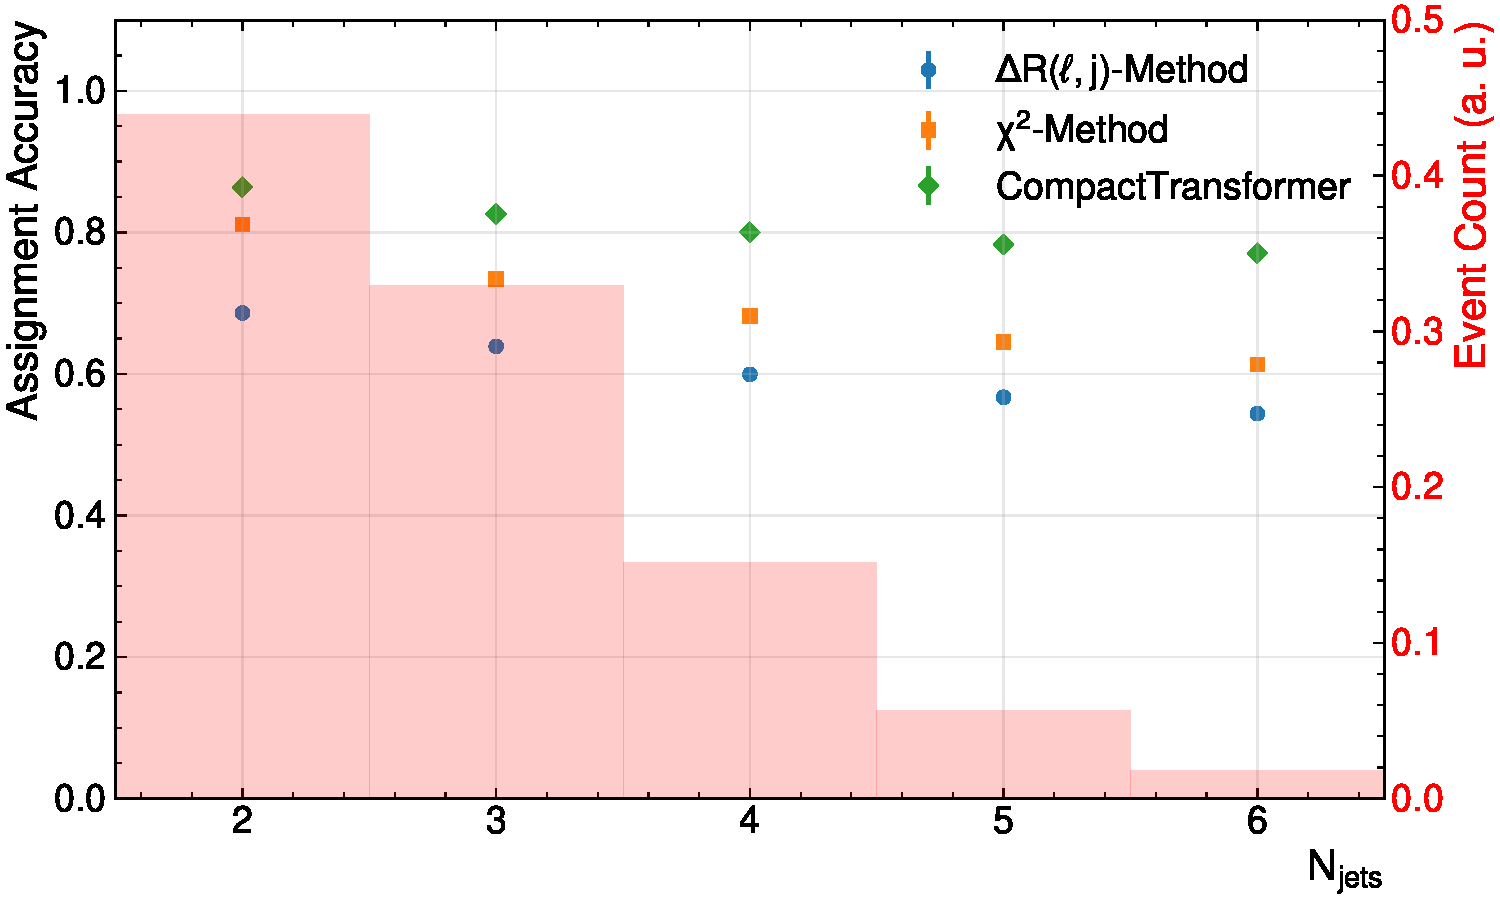
\includegraphics[width=0.7\textwidth]{plots/compact_assigner/binned_performance/N_jets/binned_accuracies_N_jets.pdf}
    \caption{Assignment accuracy as a function of the number of jets in the event for different reconstruction methods. The background histograms show of the distribution of events as a function of the number of jets. The uncertainties represent the statistical variations in the evaluation dataset.}
    \label{fig:accuracy_vs_njets}
\end{figure}%
The \Cref{fig:accuracy_vs_njets} shows the assignment accuracy for different jet multiplicities for the different methods. It can be observed, that the CompactTransformer outperforms the baseline-methods in all bins. For all methods, the performance drops with an increasing number of jets. The performance drop, however, is relatively small, which can be attributed to the performance of the b-tagging. Notably, the performance of the CompactTransformer drops the least, and the difference in performance increases for higher jet numbers. This stems from the improved accuracy of the jet-selection as shown before. In the Appendix, the \Cref{fig:selection_accuracy_vs_n_jets} shows the selection accuracy binned in the same way. It can be seen that the CompactTransformer does a much better job at selection the correct jets for events with a higher jet multiplicity. It was found, that this is the primary cause for differences in assignment accuracy with respect to the jet-multiplicity. The efficiency of assigning correctly selected jets seems to be mostly independent of the jet-multiplicity.
\begin{figure}[ht]
    \centering
    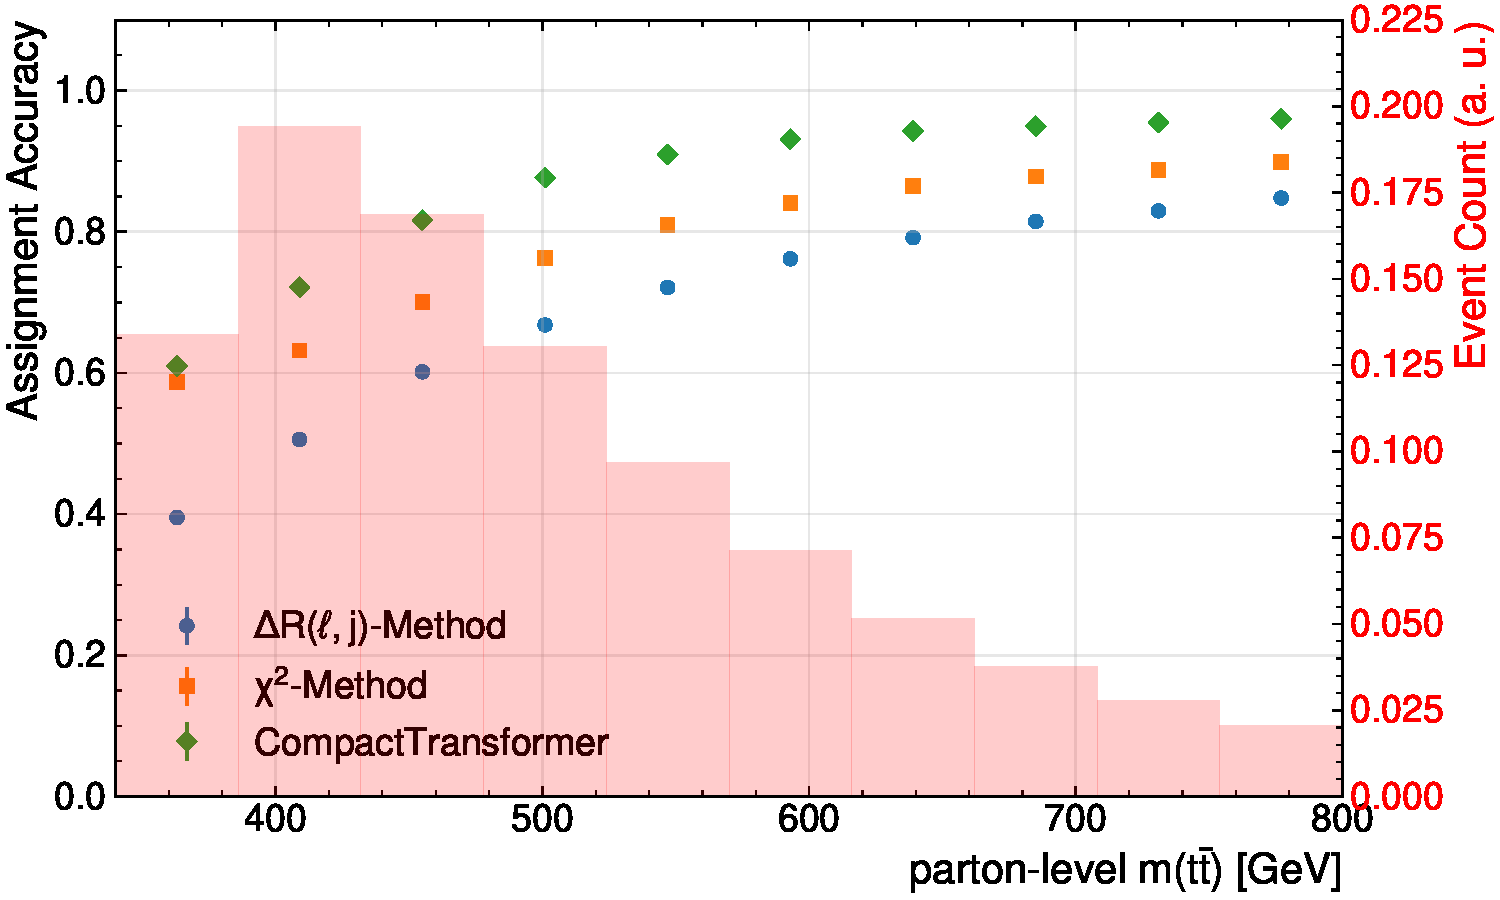
\includegraphics[width=0.7\textwidth]{plots/compact_assigner/binned_performance/truth_ttbar_mass/binned_accuracies_truth_ttbar_mass.pdf}
    \caption{This plot shows the assignment accuracy in bins of the true invariant mass of the top-quark pair.}
    \label{fig:accuracy_vs_mttbar}
\end{figure}
\Cref{fig:accuracy_vs_mttbar} shows the assignment accuracy as a function of the parton-level $m(t\bar{t})$. All methods show a similar behaviour; the accuracy drops for low invariant masses and seems to saturate for high invariant masses. For the CompactTransformer, the saturated performance in the high invariant mass regime almost approaches unity, marking near perfect reconstruction. On the other end of the spectrum, the performance drops to around 0.6 near the \ttbar-production threshold. For these low-mass events, the CompactTransformer and the $\chi^2$-Method appear to be almost on-par. In general, this indicates that the $\chi^2$-Method is the leasts sensitive to $m(t\bar{t})$, while the $\Delta R(\ell,j)$-Method seems to be most sensitive. One can consider the conditional probability to make a correct assignment, given that the correct jets were selected. For this situation, the assignment reduces to a binary problem in the dilepton case, as jets can only be assigned to bottom- or antibottom-quark respectively. According to the Bayes' theorem, this probability can be computed by dividing the assignment accuracy with the selection accuracy.
\begin{figure}[ht]
    \centering
    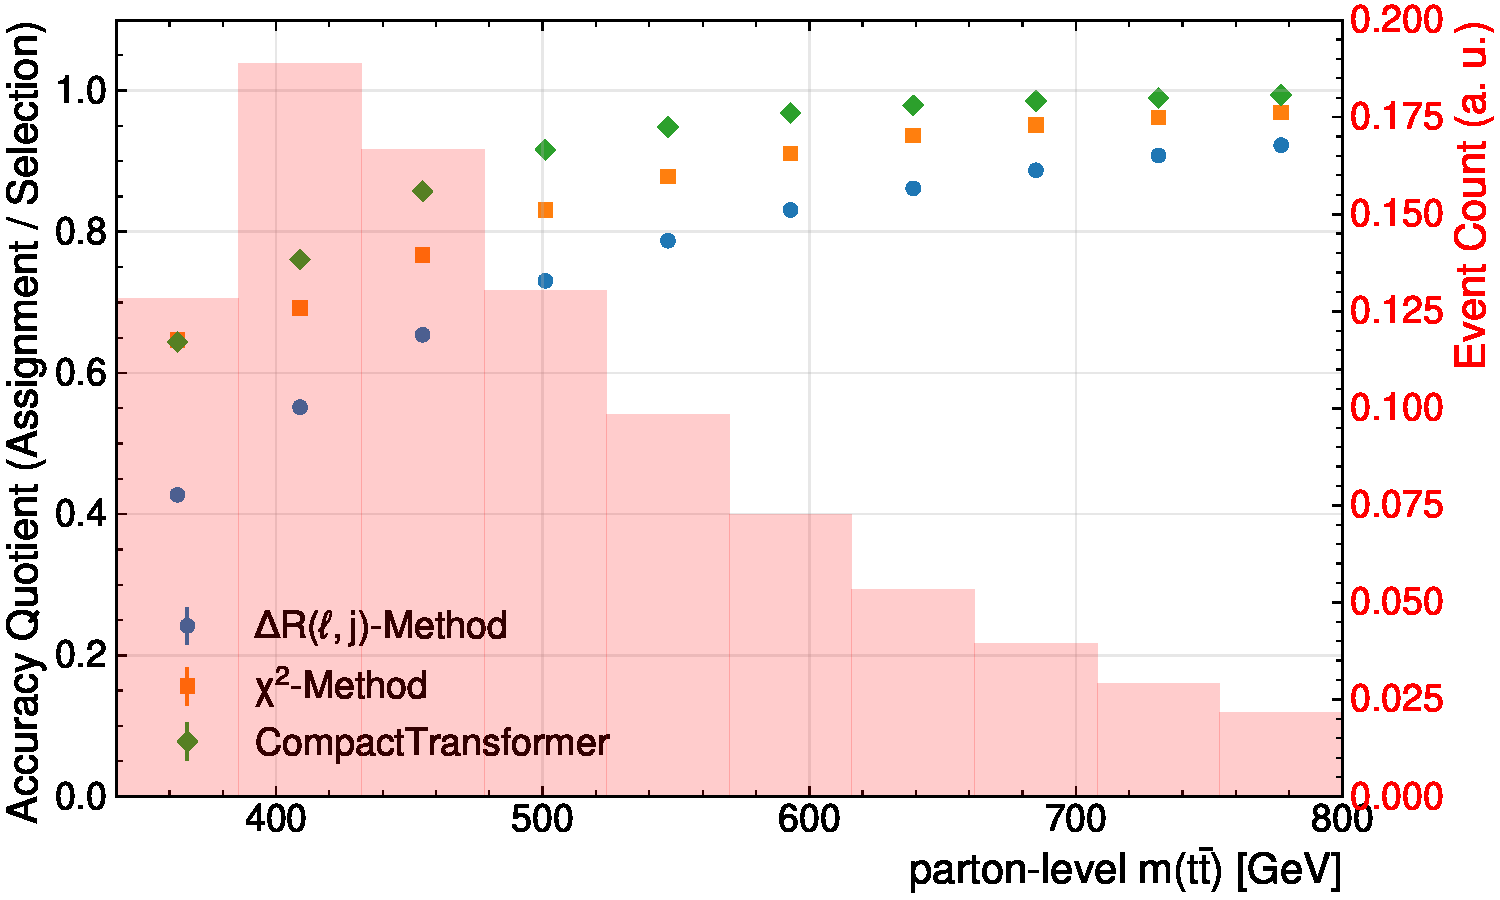
\includegraphics[width=0.7\textwidth]{plots/compact_assigner/binned_performance/truth_ttbar_mass/binned_accuracy_quotients_truth_ttbar_mass.pdf}
    \caption{Quotient of assignment and selection accuracy computed in bins of the parton-level $m(t\bar{t})$.}
    \label{fig:accuracy_quotient_vs_mttbar}
\end{figure}
The corresponding plot showing this probability for the different methods, binned in parton-level $m(t\bar{t})$, is displayed in \Cref{fig:accuracy_quotient_vs_mttbar}. This investigation allows to separate the process of actually assigning the selected jets. One thing one to note, is that the $\Delta R(\ell,j)$-Method has a performance below $0.5$ for the lowest bin, meaning that it performs worse than a random assignment in this bin. This suggests, that the topology of the particles in this region actually disfavours assigning jets based on proximity. \Cref{fig:deltaR_pairing} in the Appendix clearly shows the difference in angular distance for correct and incorrect jet-lepton pairing between the inclusive sample and the near-threshold region.
Another observation is, that in the lowest bin, the CompactTransformer and $\chi^2$-Method are completely on par for this metric. Generally, it can be concluded, that the region close to the production threshold features a particularly challenging topology for the assignment of jets. One particular property of the events close to the production-threshold is, that they feature smaller separation of the leptons. The double-binned distribution of events in \Cref{fig:feature_2d_mttbar_dR_l1l2} shows that events with lower $m(t\bar{t})$ tend to have more collimated leptons, whereas they are more separated for more energetic events.
Since the angular separation of the leptons is suspected to worsen the performance of the events, its impact on the individual methods is investigated.
\begin{figure}[ht]
    \centering
    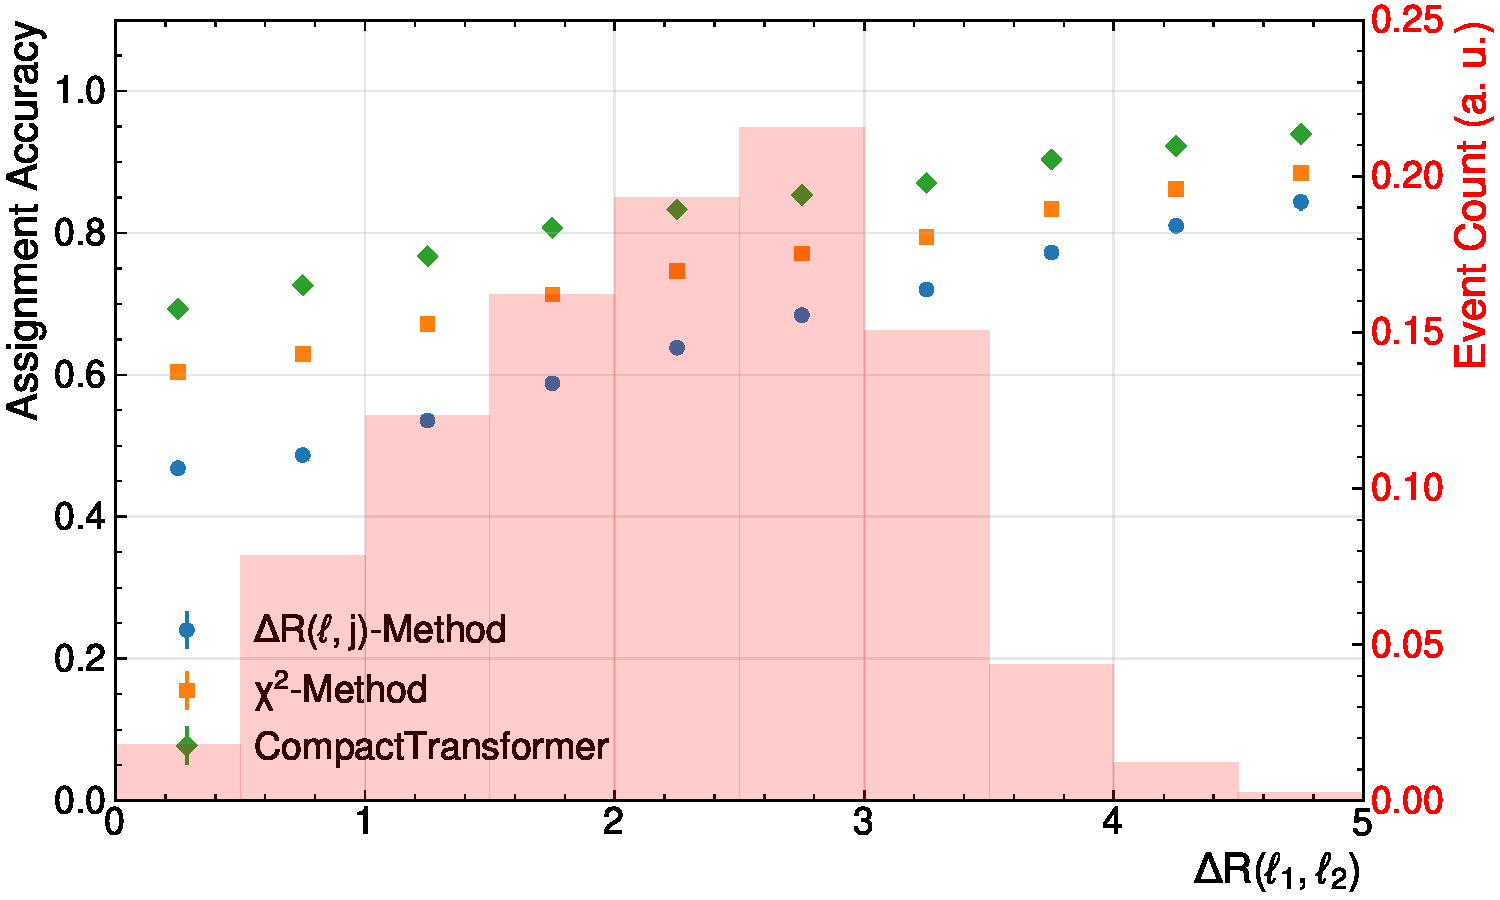
\includegraphics[width=0.7\textwidth]{plots/compact_assigner/binned_performance/dR_l1l2/binned_accuracies_dR_l1l2.pdf}
    \caption{Assignment accuracy binned in the angular distance between the two leptons of the events $\Delta R(\ell_1,\ell_2)$.}
    \label{fig:accuracy_vs_dr_l1l2}
\end{figure}
\Cref{fig:accuracy_vs_dr_l1l2} shows the assignment accuracy in bins of the angular distance $\Delta R(\ell_1,\ell_2)$ between the two leptons. All methods suffer losses in performance for events with close leptons. Interestingly, however, even for the smallest\footnote{Due to the so-called overlap-removal, which removes overlapping objects from the events, there is a cut-off at $\Delta R<0.3$. This technique accounts for the fact that in a detector objects that coincidence cannot be separated.} angular separation the performance is still above the one for near-threshold events.
A combined comparison of both variables' impact is shown in \Cref{fig:accuracy_2d_mttbar_dR_l1l2} in the Appendix. The double-binned accuracy reveals, that the invariant mass $m(t\bar{t})$ seems to have a much stronger impact on the performance, than the angular separation alone.



\section{Neutrino Regression}
\label{sec:neutrino-regression}



\section{Variable Reconstruction}
\label{sec:variable-reconstruction}



\section{Region Specific Performance}
\label{sec:region-specific-performance}




\chapter{Data-Driven Validation Studies}
\label{chap:physics-analysis}

\section{Run 2 Data Sample}
\label{sec:run-2-data-sample}

\section{Analysis Setup}
\label{sec:analysis-setup}
\begin{table}[h]
\centering
%
\caption{Summary of event selection criteria for the SRs and CRs in the analysis. The letter $\ell$ refers to $e$ and $\mu$, and OSSF refers to a lepton pair with opposite charge and the same flavour.}
\begin{tabular}{c|c|c}
\toprule
\textbf{SRs} & \textbf{CR-Z} & \textbf{CR-Fakes} \\
\midrule
\multicolumn{3}{c}{$=2\ell$ with $\pt(\ell) \geq 10~\GeV$} \\
\multicolumn{3}{c}{$\geq 1$ trigger-matched lepton with $\pt \geq 25/27/28~\GeV$} \\
\multicolumn{3}{c}{$\geq 2$ jets with $\pt \geq 25~\GeV$} \\
\multicolumn{3}{c}{$\geq 1$ $b$-tagged jet (70\% efficiency WP)} \\
\multicolumn{3}{c}{$m_{\ell\ell} \geq 15~\GeV$ for $ee$ and $\mu\mu$ events} \\
\multicolumn{3}{c}{$m_{t\bar{t}} \leq 500~\GeV$} \\
\midrule
\multicolumn{2}{c|}{$\met \geq 60~\GeV$ for OSSF events} & --- \\
\midrule
$\ell^\pm\ell^{'\mp}$ & $e^\pm e^\mp/\mu^\pm\mu^\mp$ & $\ell^\pm\ell^{'\pm}$ \\
$|m_{\ell\ell} - m_Z| \geq 10~\GeV$ & $|m_{\ell\ell} - m_Z| \leq 10~\GeV$ & $|m_{\ell\ell} - m_Z| \geq 10~\GeV$ \\
%
%
%
%
\bottomrule
\end{tabular}
\label{tab:selection_2l}
\end{table}


\section{Results}
\label{sec:results}

\chapter{Conclusion}
\label{chap:conclusion}
\section{Summary}
\label{sec:summary}
Many open questions and insightful measurements can be performed
using dileptonic decays of top-quarks. While the channel has a low
branching ratio, it can over a particularly clean event environments.
The recent analyses of quantum effects and quasi-bound state effects
near the production threshold, have motivated further investigations
into this region. The dileptonic decays provide unique and
unparalleled precision for tests of spin-structures in the involved
physics-processes.
Despite offering a clean environment for analyses, the channel has it
own challenges. The presence of two neutrinos from the leptonic decay
of the $W$-bosons leaves $6$ unknown momenta components. Furthermore,
selecting and assigning the $b$-jets to their parent top-quarks
provides additional ambiguities. While the neutrino regression has
been studied in the past, the assignment of the neutrinos is not only
understudied, but the two tasks are also inherently intertwined. Many
variables that are essential for the measurements of the internal
structure, require a full reconstruction of the top-quarks four
momenta. Thus, the reconstruction and its performance is an essential
aspect for the sensitive of many studies of the top-quark pairs.

To address the jet-assignment, a transformer-based machine-learning
model was developed and trained. Different architectures and layouts
have been tested, but showed very similar performance -- despite
incorporating distinct symmetries of the kinematic objects. The
developed model was found to provide substantial improvement in the
efficiency of the jet-assignment. This increased accuracy propagates
to smaller errors for the reconstruction, and lastly also improved
resolutions for these variables, which ultimately increases the
sensitivity of measurements.
Apart from the general improvements that were observed, a more
detailed investigation revealed which regions of phase-space benefit
the most from the reconstruction using the ml-approach.
Notably, the region near the production-threshold proofed to be
particularly challenging. For this region, no substantial improvement
in accuracy compared to the baseline-methods was observed. Some
kinematic features, making reconstruction in this regime difficult
could be identified, but a share of these effects remains elusive.

To further improve the event reconstruction, and resolve the
interdependencies of the two tasks, a model capable to provide
jet-assignment and neutrino regression was developed. The underlying
model architecture extended the previous layout by an additional
output head for the neutrino momenta. While one initial aim was to
resolve the interdependency, the improvements by a combined approach
were limited. Comparing the performance of models performing only
either of the two tasks with the multi-task model, showed no
improvement for accuracy of jet-assignment and only minor
improvements for the regression.
It was, however, found that some cross-talk between the tasks exist.
Therefore, already existing tools that provide neutrino-regression,
both analytical and ml-based, can be expected to provide valuable
information on the jet-assignment.
Further, the developed methods could improve both the error of the
neutrino regression, and the resolution of derived variables -- such
as spin-sensitive markers, and the invariant mass of the
\ttbar-system. However, despite the improvement in the variable
reconstruction, the model was found to come with strong biases in the
reconstructed variables, which led to significant distortions in the
distributions of reconstructed variables. Some measures to correct
such distortions could be identified and discussed. Yet, the
underlying cause for these effects was found to be, most likely, the
probabilistic nature of the neutrino momenta. Since the neutrinos are
inherently underdetermined, they are most accurately modelled by a
conditional probability density. Training a regression model
collapses the output to the mean of this probability distribution,
which can lead to biases in the computation of non-linear variables.
This can be mitigated by modelling and propagating the conditional
density from the neutrino momenta to reconstructed variables and
averaging over their distributions instead. Generally, this would
provide a more complete representation of the kinematics.

Lastly, the performance of the methods developed here was showcased
by reproducing the analysis of bound-state effects at the production
threshold in a highly simplified setting. An Asimov-fit, aimed to
assess the potential impact on an analysis, found that the
uncertainties associated with the signal strength are significantly
decreased by methods with enhance resolution such as $\nu^2$-Flows
and the MultiModalTransformer, as it was presented in this work. The
latter is able to achieve a 3-fold increase in the significance of
the signal strength, which presents are remarkable improvement. In
practice, however, this will be limited by contributions from
systematic uncertainties. Moreover, the enhanced reconstruction of
the MultiModalTransformer comes with a stark limitation of its own:
reconstructed variables of the top-quarks such as the invariant mass
of the \ttbar-system and the spin-sensitive \chel and \chan comes
with significant biases and distortions in the shape. While it was
shown that this does not impact -- as data and simulation are
distorted in the same way, this can be critical for analyses that
extract information from the distributions directly. One notable
example is the measurement of quantum effects in Reference
\cite{atlas_entanglement}, which used the slope of the
\chel-distribution as its marker for entanglement. Hence, additional
consideration would be necessary for such an analysis. Especially the
distributions of reconstructed masses show very clearly, that this
ml-based method provides conceptually different results from other
methods, that preserve the physical constraints more consistently.
Thus, it might be necessary to investigate which method provides the
most sound results for the particular analysis, one is interested in
and adapt accordingly.

For reconstructed variables, it is always important that they are
well-modelled by the simulations. To ensure such a consistency for
the reconstruction provided by the MultiModalTransformer,
distributions of reconstructed variables such as the top-quark mass
were compared between simulation and data collected by \atlas.
Generally, a very good agreement in the distributions was found.
Highlighting that this tools can be applied to simulation as well as
event data. The distributions show the robustness of the method to be
used on data and in future analyses.

Combined with the thorough evaluation of the method's performance, it
provides a clear motivation to use an approach developed here, or a
similar one, in future research. Lastly, the combination of two
reconstruction tasks into a single model not only resolves
interdependencies but can also cut computational load. The transition
to the HL-LHC, which will increase the event number by up to one
order of magnitude, will bring additional challenges related to the
computation time of analyses. Therefore, tools that combine tasks are
becoming increasingly important as they reduce redundancies.

\section{Outlook}
\label{sec:outlook}
This thesis provided a comprehensive coverage of the strengths and
weaknesses of the methods. Based on the research conducted, new
research goals and questions have emerged.

One very important aspect this thesis highlighted was the
interdependency of the reconstruction tasks in the dilepton channel.
The analysis conducted here showed conclusively that the two tasks
are inherently linked. Thus, it is strongly encouraged that a tool
like $\nu^2$-Flows, which provides a neutrino regression, is extended
to output the assignment. This is motivated by the finding, that a
transformer trained to regress the neutrinos build an internal
understanding about the assignment structure. Hence, a tool should
generally provide both aspect. This would also increase consistency
between the assignment of jets and regression of neutrinos, which
might be lost when interfaced with additional tools.

The next open question is the aforementioned propagating of the
neutrino posterior to derived event variables. It was shown that
averaging over the posterior of event variables instead of computing
event variables from averaged momenta can lead to improvement such as
reduced biases and enhanced resolutions. Furthermore, it might be
useful to incorporate such a posterior of an event variable into a
fit or perhaps the uncertainty. This would provide a more
comprehensive description of the underdetermined neutrinos.

Going one step further, it is also possible to incorporate the
probability distribution of reconstructed variables to the
loss-function itself. Using automatic differentiation to compute the
Jacobian, the probability density of the neutrinos can be transformed
to the probability density of the reconstructed variables. This would
allow one to optimise the model with respect to the variables, that
one is eventually interested in -- i.e. reconstructed variables such
as $m(t\bar{t})$, \chel, or \chan. Similarly, regression these
variables directly could also be investigated. In case where the
interpretability is less important than the separation power of
variable, one might also consider training a discriminator. One
notable example is the search for contributions from non-relativistic
bound state effects. For such an analysis, a discriminating neural
network can be trained to separate events from both states and this
provide one, or possibly multiple, sensitive variables.

Lastly, as it was shown that the tool can provide improvements for
the analyses involving dileptonic decays of top-quark pairs, it can
be expected to be used in future investigations. The most notable one
remains the investigation of bound-state effects at the
\ttbar-production threshold. For a measurement of the cross-section,
a significant improvement in the uncertainty is projected by the use
of the MultiModalTransformer. To facilitate an application in a
measurement by \atlas, the tool was made available in the central
software used for top-related analyses: TopCPToolkit \cite{topcptoolkit}.
Combined with the increased statistics offered by the \LHCruniii in
the near future, very promising progress in the understanding of
these effects can be expected.


\appendix
\chapter{Additional Plots}
\label{chap:add-plots}

\section{Data Feature Plots}
\begin{figure}[H]
    \centering
    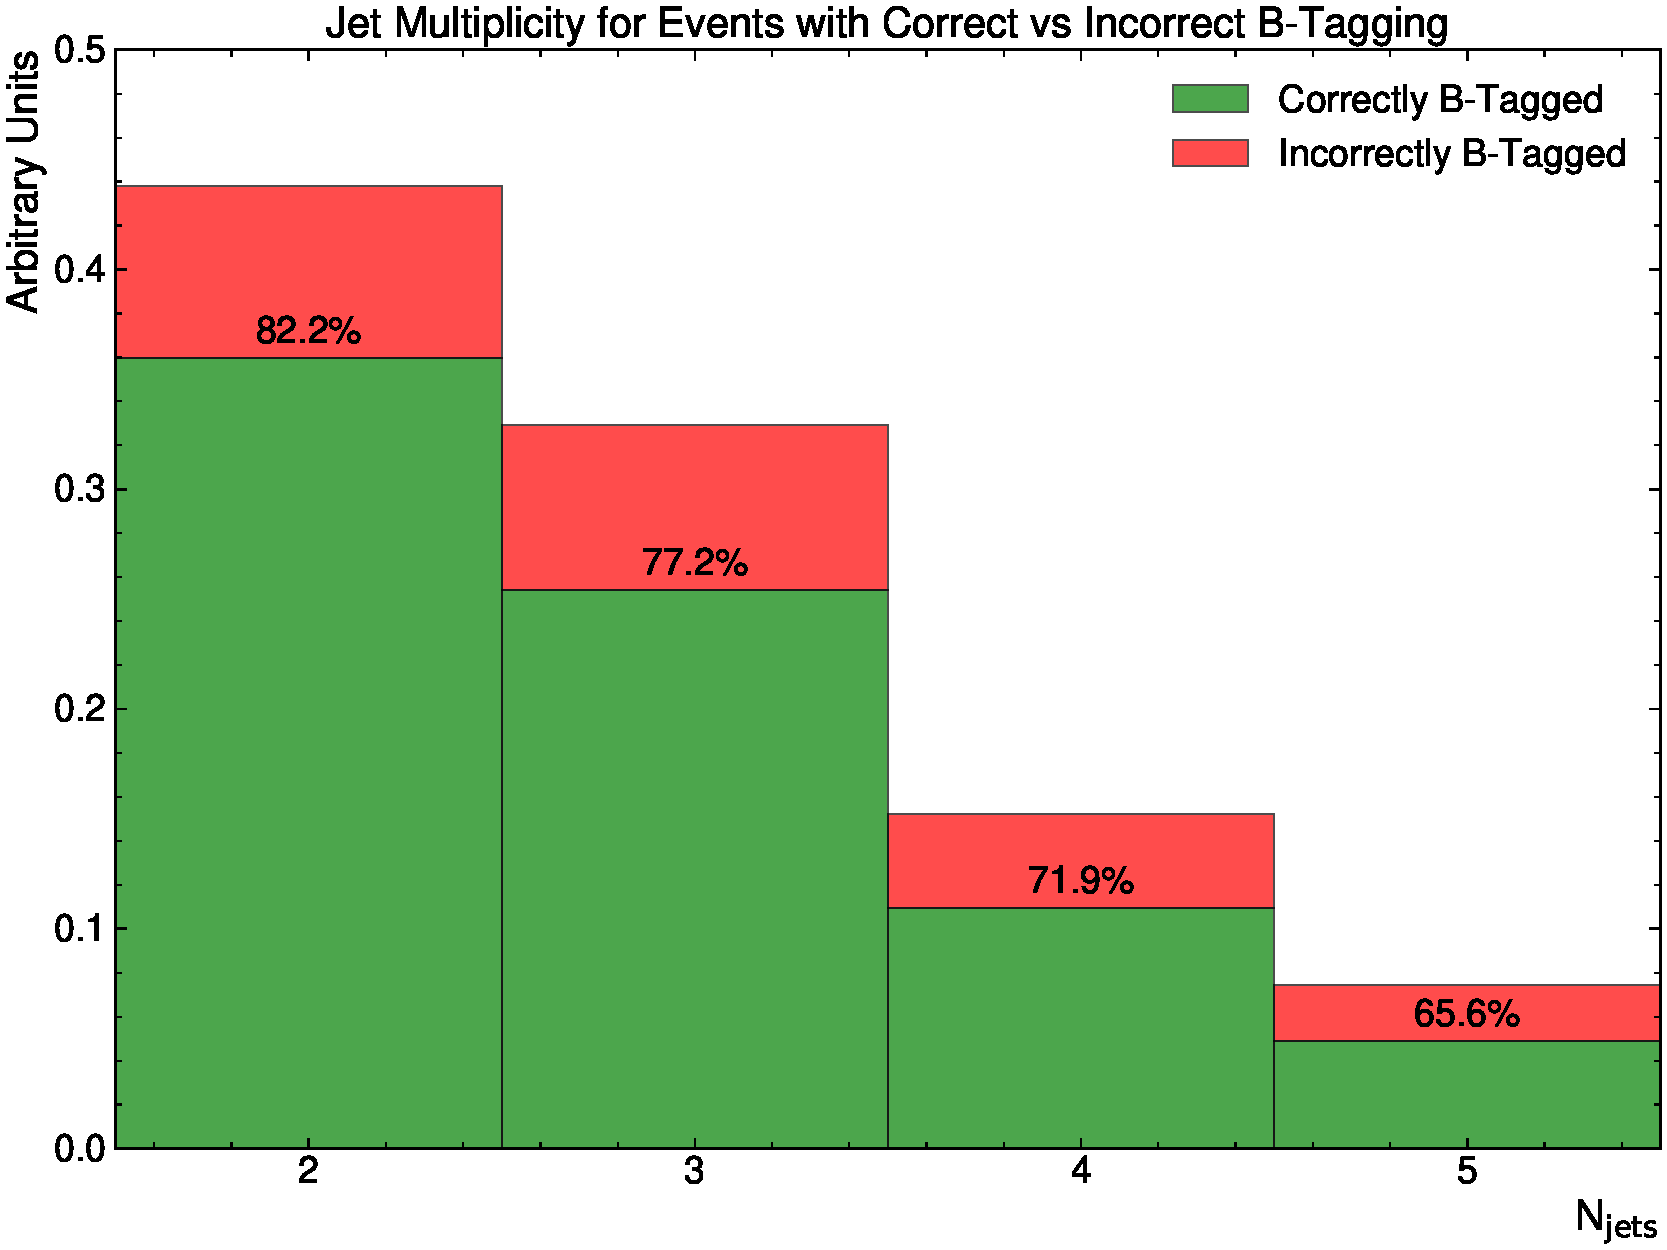
\includegraphics[width=0.7\textwidth]{plots/feature_plots/btagging_performance_by_jet_multiplicity.pdf}
    \caption{This plot shows the b-tagging performance for different numbers of jets in the event. For each jet multiplicity, the number of events, with only jets from top-decays being b-tagged }
\end{figure}

\subsubsection{Threshold Topology}
\label{sec:threshold_topology}
\begin{figure}[H]
    \centering
    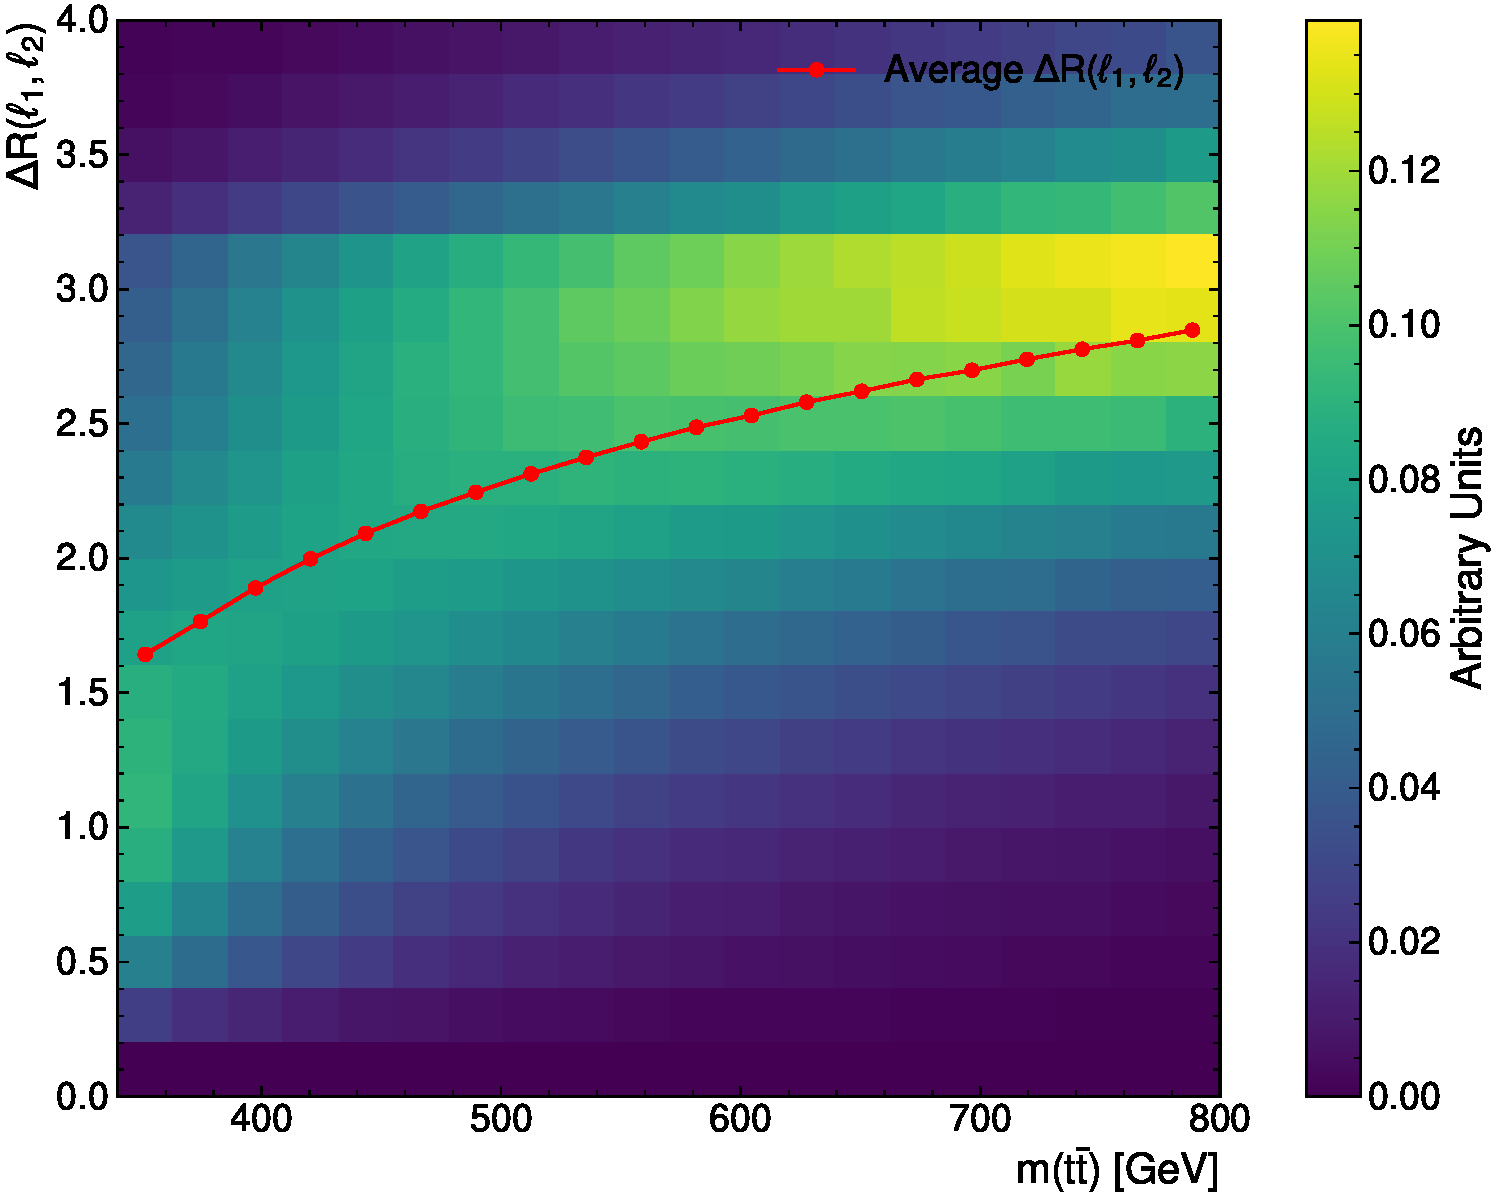
\includegraphics[width=0.7\textwidth]{plots/feature_plots/ttbar_mass_vs_dR_l1l2.pdf}
    \caption{This plot shows the distribution of events binned in the parton-level $m(t\bar{t})$ and the angular distance $\Delta R(\ell_1,\ell_2)$.}
    \label{fig:feature_2d_mttbar_dR_l1l2}
\end{figure}


\begin{figure}[H]
    \begin{subfigure}{0.49\textwidth}
        \centering
        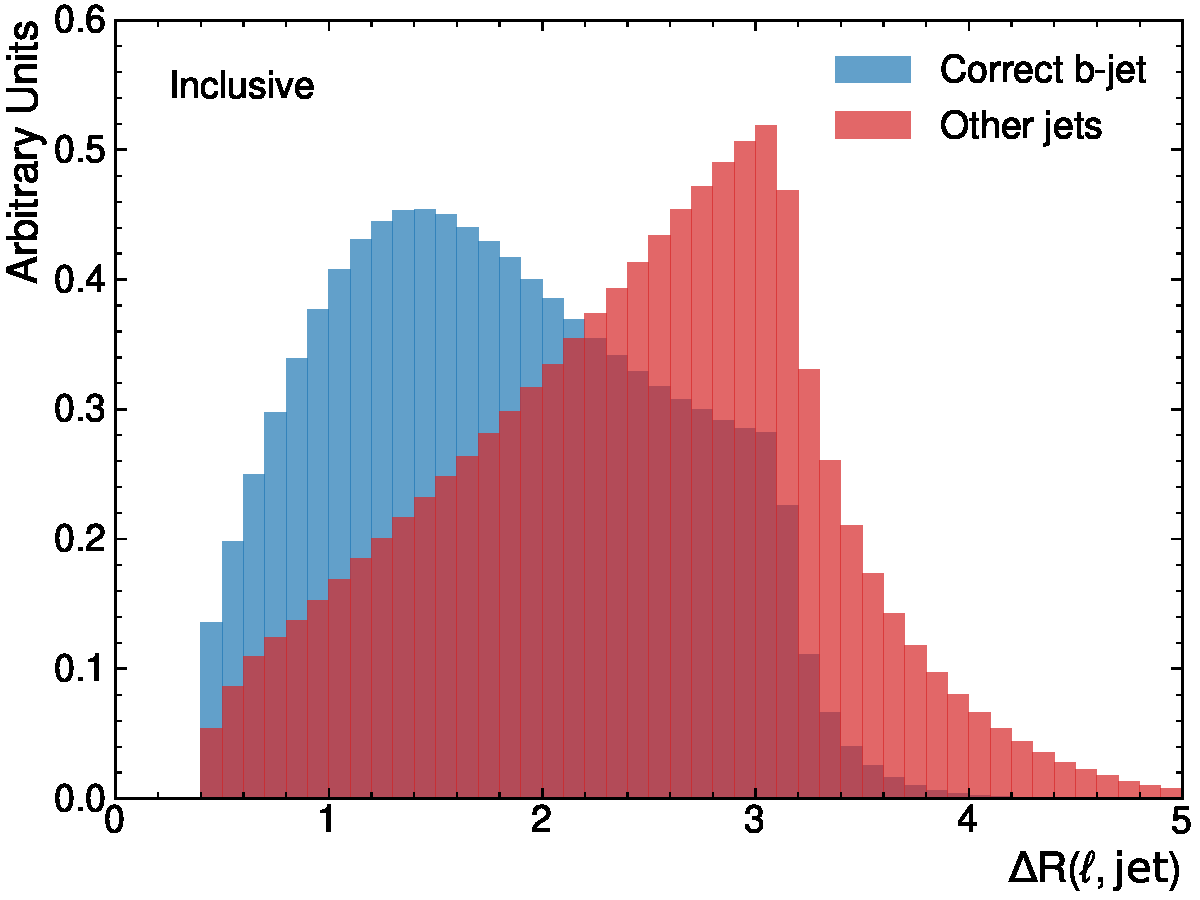
\includegraphics[width=1.0\textwidth]{plots/feature_plots/relational_jet_lepton_deltaR_distribution.pdf}
        \caption{Inclusive}
        \label{fig:deltaR_pairing:inclusive}
    \end{subfigure}
    \begin{subfigure}{0.49\textwidth}
        \centering
        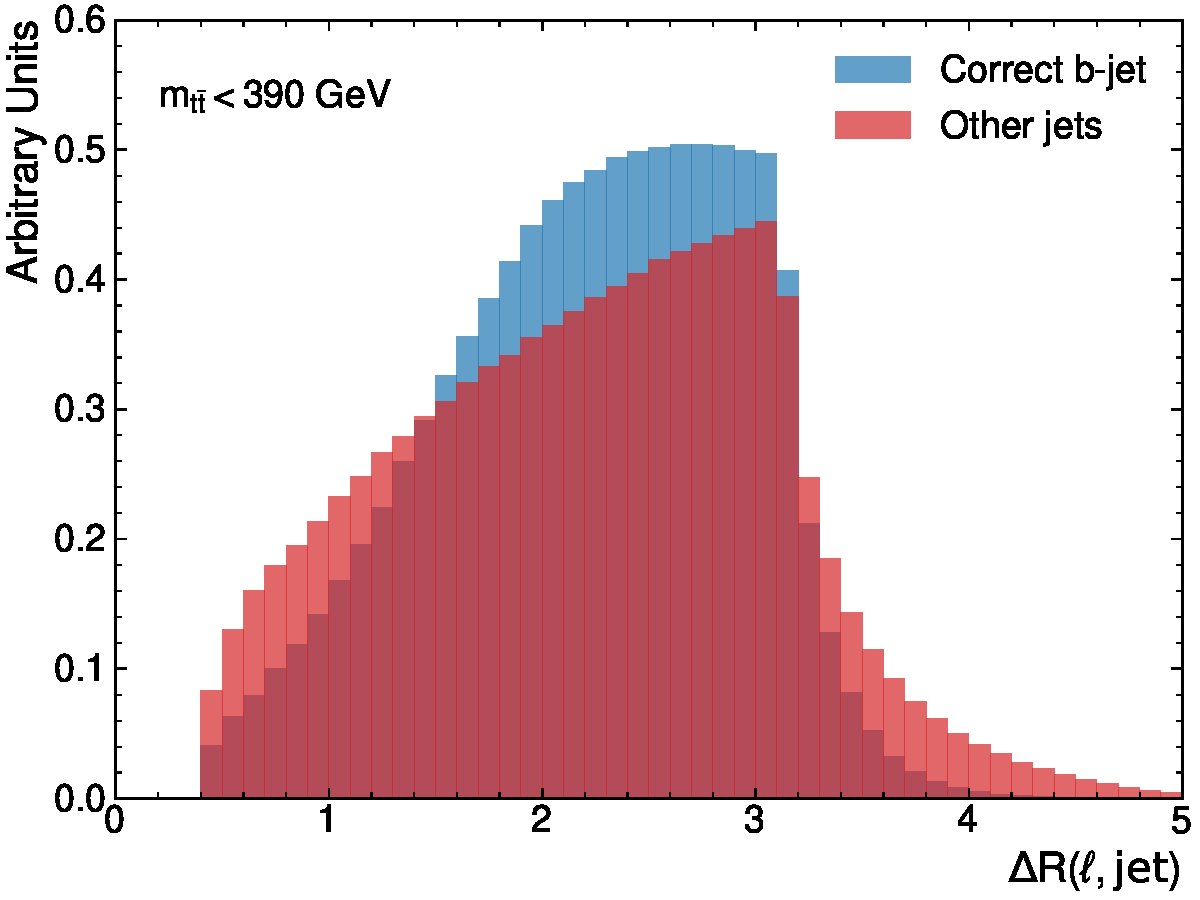
\includegraphics[width=1.0\textwidth]{plots/feature_plots/relational_jet_lepton_deltaR_distribution_m_tt_390GeV.pdf}
        \caption{Near-Threshold}
        \label{fig:deltaR_pairing:threshold}
    \end{subfigure}
    \caption{Distribution of $\Delta R(\ell,j)$ for correct and incorrect pairing of jets and leptons. Evaluated on the full sample in \subrefb{fig:deltaR_pairing:inclusive} and near-threshold in \subrefb{fig:deltaR_pairing:threshold}.}
    \label{fig:deltaR_pairing}
\end{figure}

\begin{figure}[H]
    \begin{subfigure}{0.49\textwidth}
        \centering
        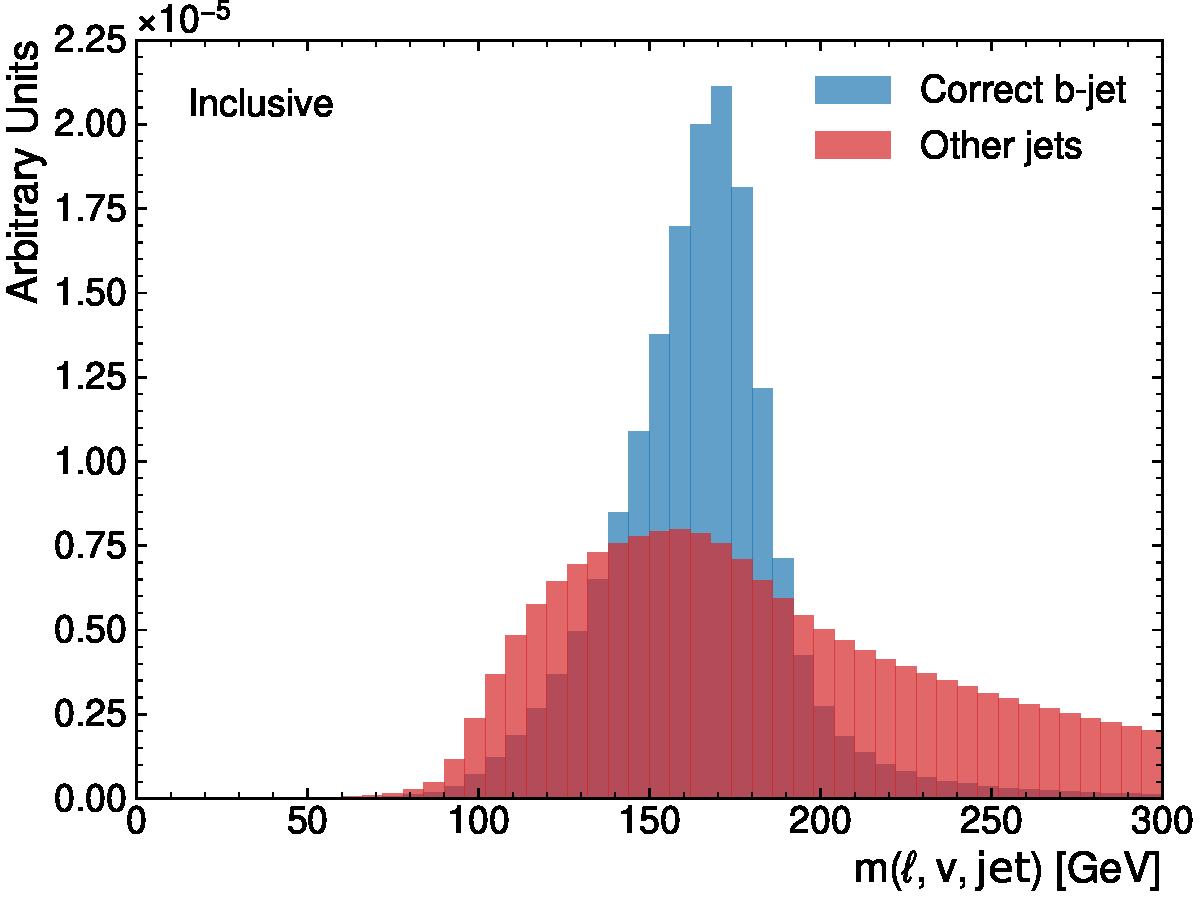
\includegraphics[width=1.0\textwidth]{plots/feature_plots/relational_jet_lepton_full_inv_mass_distribution.pdf}
        \caption{Inclusive}
        \label{fig:invariant_mass_pairing:inclusive}
    \end{subfigure}
    \begin{subfigure}{0.49\textwidth}
        \centering
        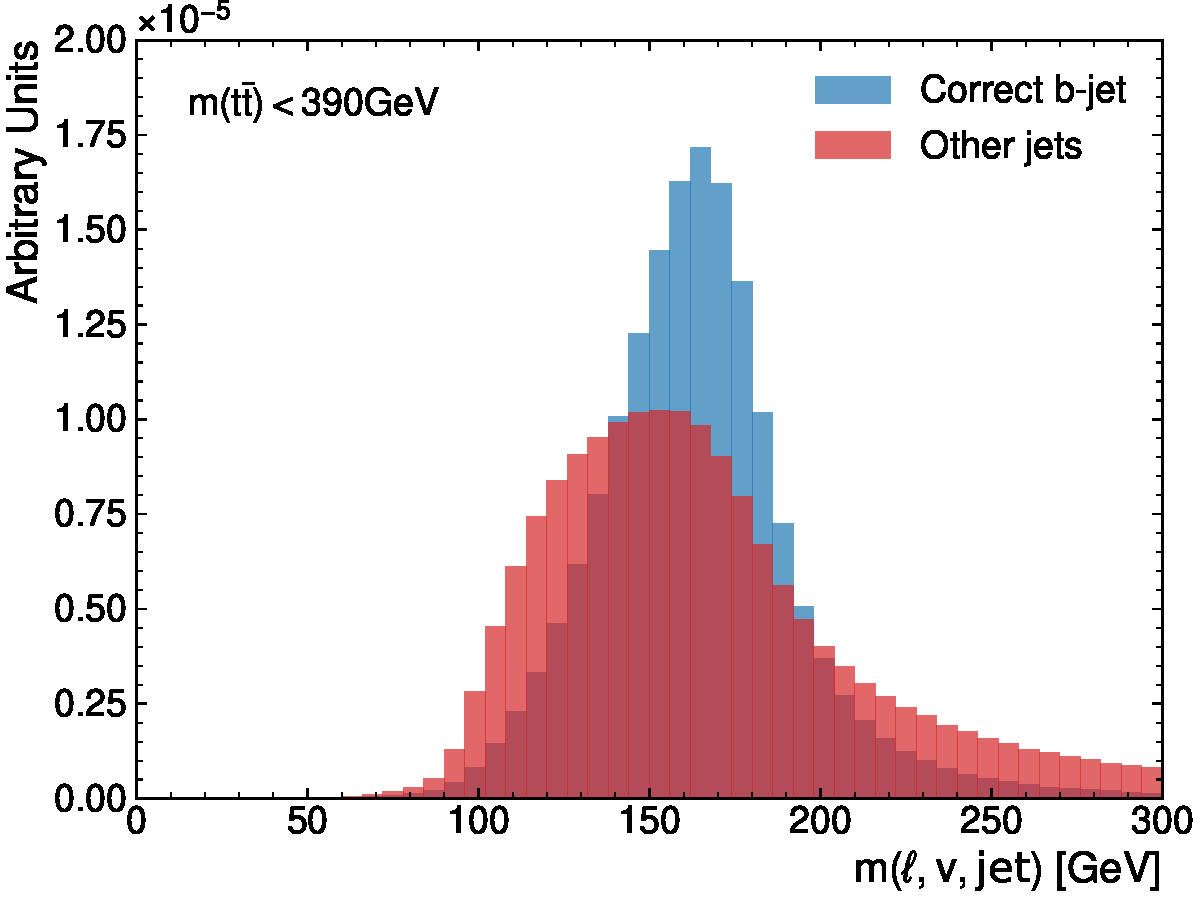
\includegraphics[width=1.0\textwidth]{plots/feature_plots/relational_jet_lepton_full_inv_mass_distribution_m_tt_390GeV.pdf}
        \caption{Near-Threshold}
        \label{fig:invariant_mass_pairing:threshold}
    \end{subfigure}
    \caption{Distribution of $m(\ell,\nu, j)$ for correct and incorrect pairing of jets and leptons. Evaluated on the full sample in \subrefb{fig:invariant_mass_pairing:inclusive} and near-threshold in \subrefb{fig:invariant_mass_pairing:threshold}.}
    \label{fig:invariant_mass_pairing}
\end{figure}



\section{Hyperparameter Optimisation Results}
\label{sec:hyperparams}

\subsection{FeatureConcatTransformer}
\begin{figure}[H]
    \begin{subfigure}{1.0\textwidth}
        \centering
        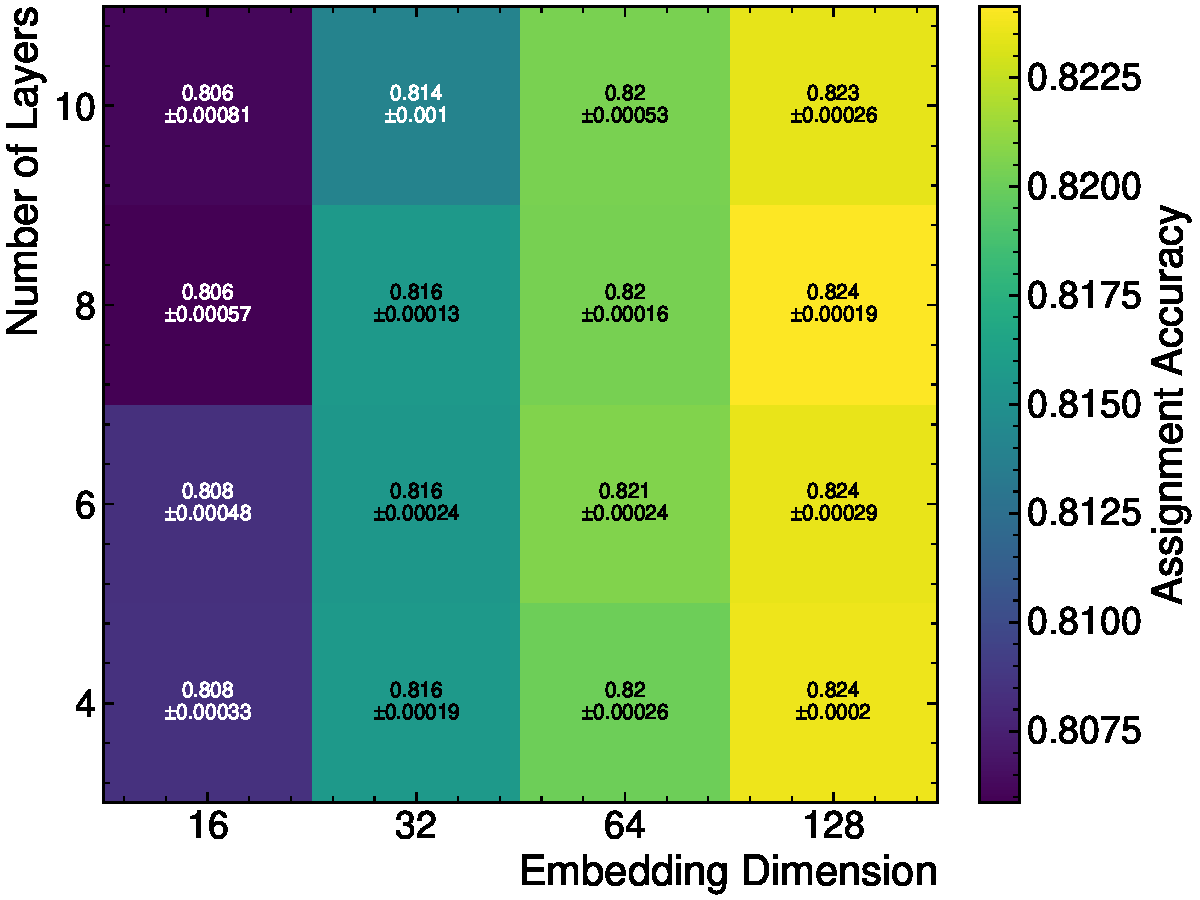
\includegraphics[width=0.7\textwidth]{plots/hyperparams_assignment/FeatureConcatTransformer_assignment_accuracy_embedding_dimension_vs_num_layers.pdf}
        \caption{Assignment Accuracy}
        \label{fig:hyperparams_fct_acc}
    \end{subfigure}
    \begin{subfigure}{1.0\textwidth}
        \centering
        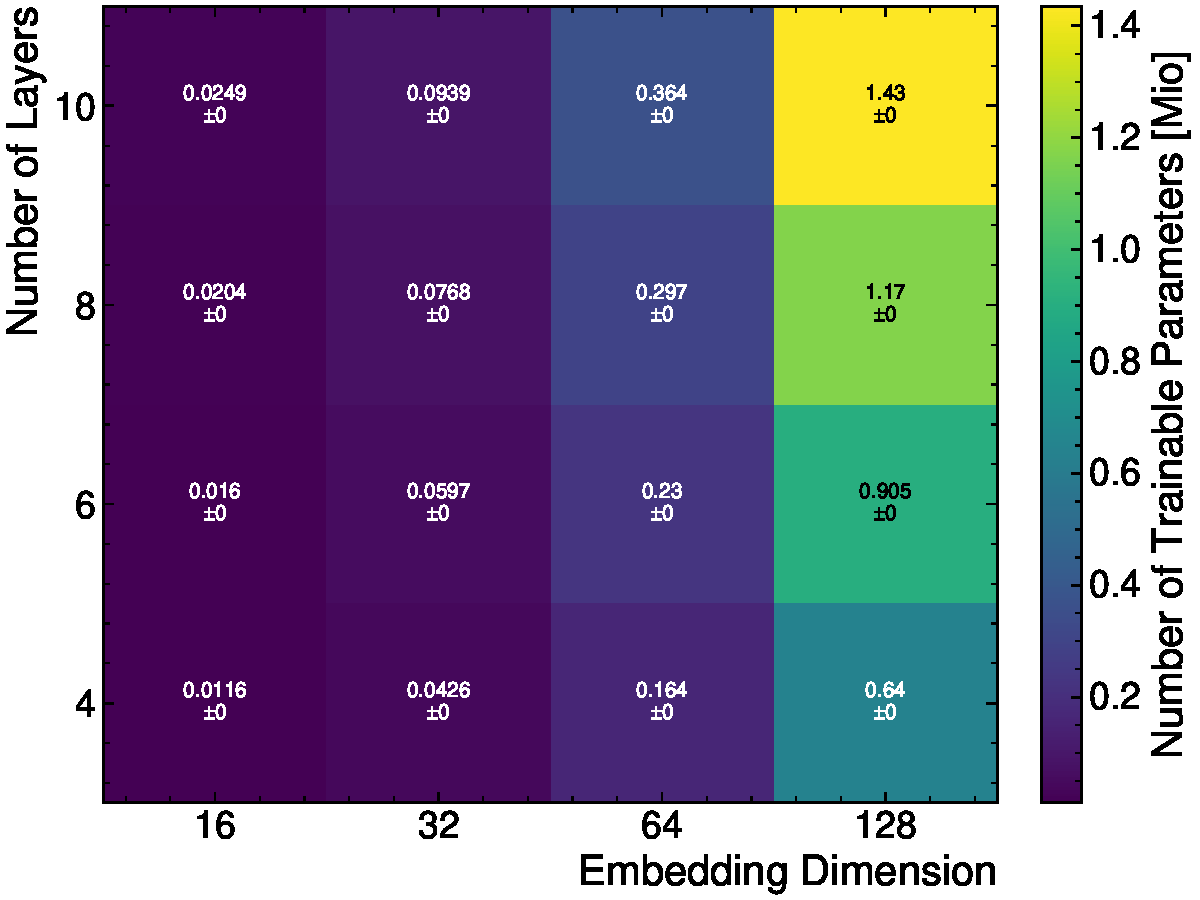
\includegraphics[width=0.7\textwidth]{plots/hyperparams_assignment/FeatureConcatTransformer_num_trainable_parameters_embedding_dimension_vs_num_layers.pdf}
        \caption{Number of Trainable Parameters}
        \label{fig:hyperparams_fct_params}
    \end{subfigure}
    \caption{The Figures \subrefb{fig:hyperparams_fct_acc} and \subrefb{fig:hyperparams_fct_params} show the assignment accuracy and the number of trainable parameters of the FeatureConcatTransformer architecture as a function of the embedding dimension and the number of transformer layers.}
    \label{fig:hyperparams_fct}
\end{figure}

\subsection{CrossAttentionTransformer}
\begin{figure}[H]
    \begin{subfigure}{1.0\textwidth}
        \centering
        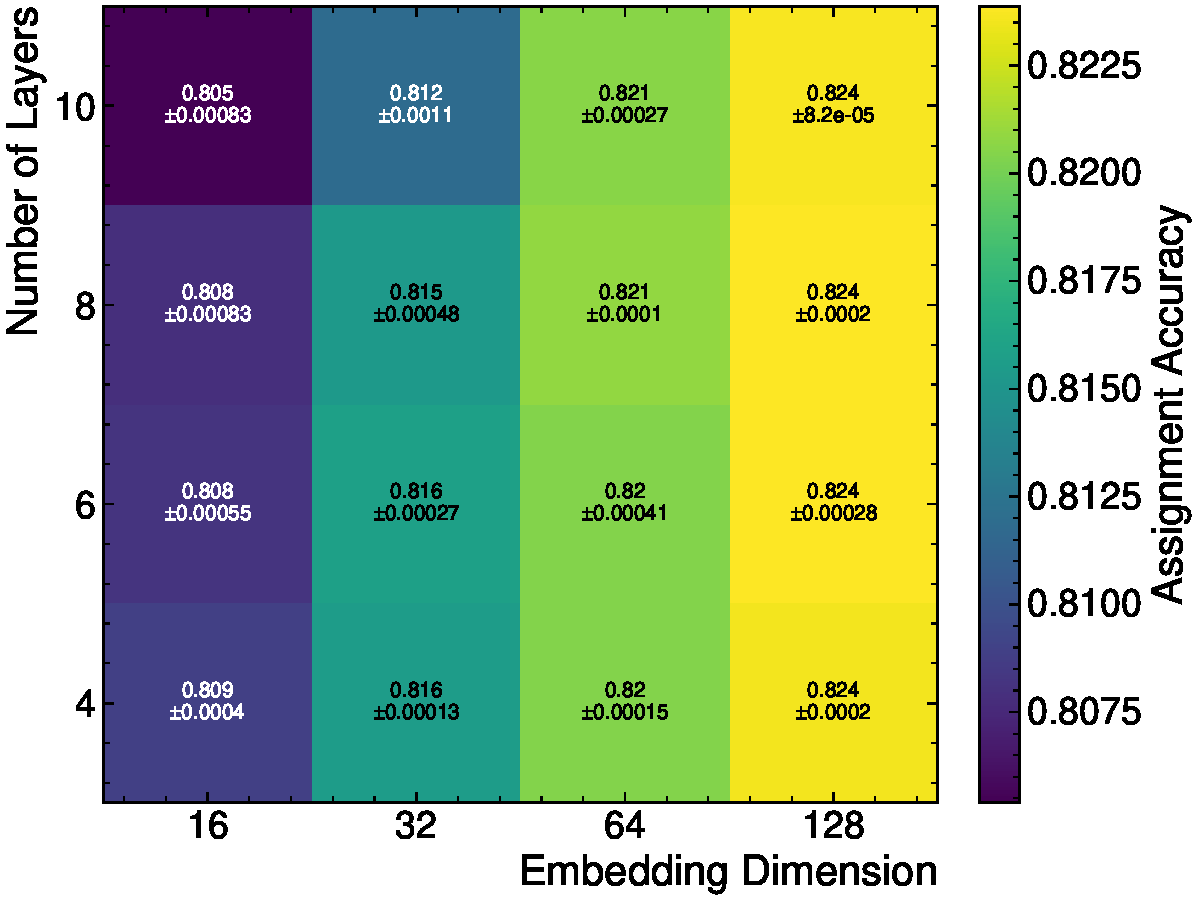
\includegraphics[width=0.7\textwidth]{plots/hyperparams_assignment/CrossAttentionTransformer_assignment_accuracy_embedding_dimension_vs_num_layers.pdf}
        \caption{Assignment Accuracy}
        \label{fig:hyperparams_cat_acc}
    \end{subfigure}
    \begin{subfigure}{1.0\textwidth}
        \centering
        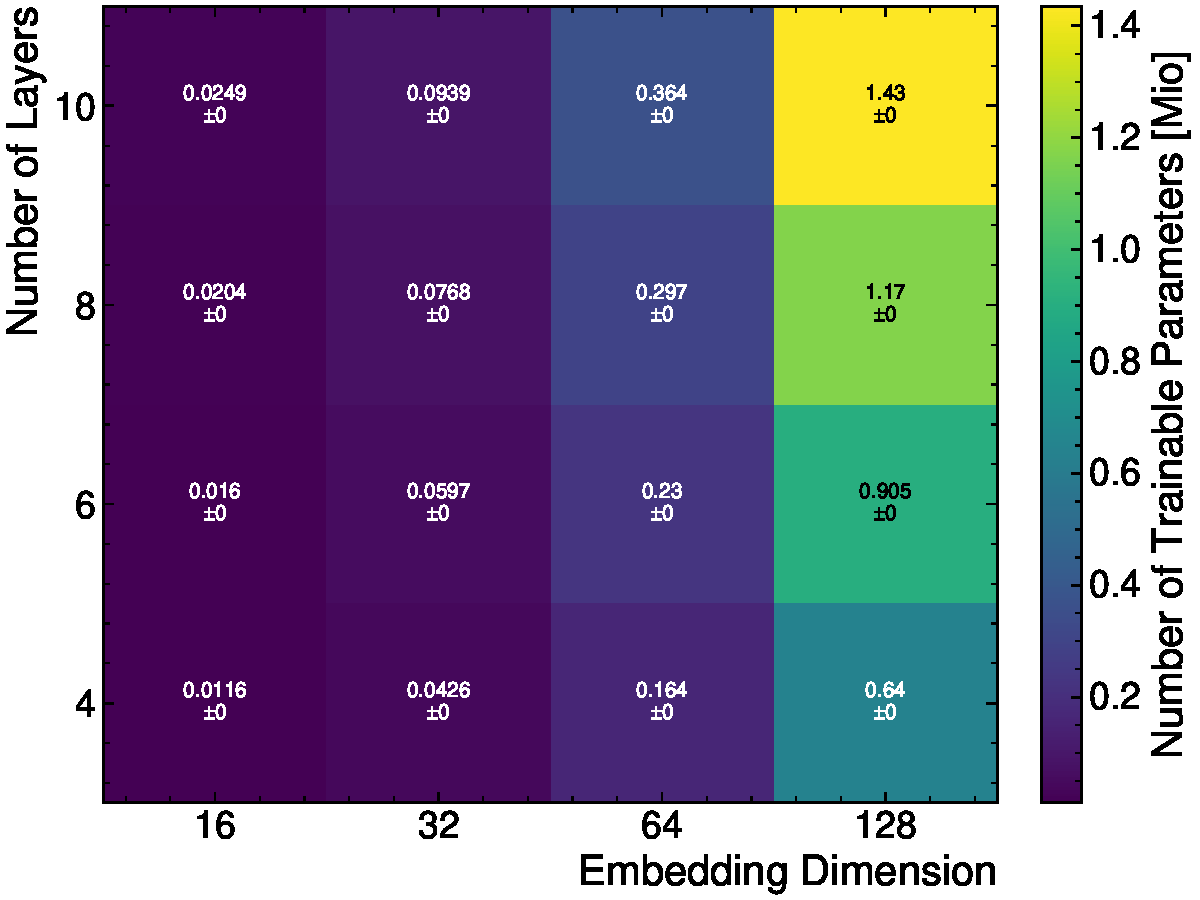
\includegraphics[width=0.7\textwidth]{plots/hyperparams_assignment/CrossAttentionTransformer_num_trainable_parameters_embedding_dimension_vs_num_layers.pdf}
        \caption{Number of Trainable Parameters}
        \label{fig:hyperparams_cat_params}
    \end{subfigure}
    \caption{The Figures \subrefb{fig:hyperparams_cat_acc} and \subrefb{fig:hyperparams_cat_params} show the assignment accuracy and the number of trainable parameters of the CrossAttentionTransformer architecture as a function of the embedding dimension and the number of transformer layers.}
    \label{fig:hyperparams_cat}
\end{figure}

\subsection{CompactTransformer}
\begin{figure}[H]
    \begin{subfigure}{1.0\textwidth}
        \centering
        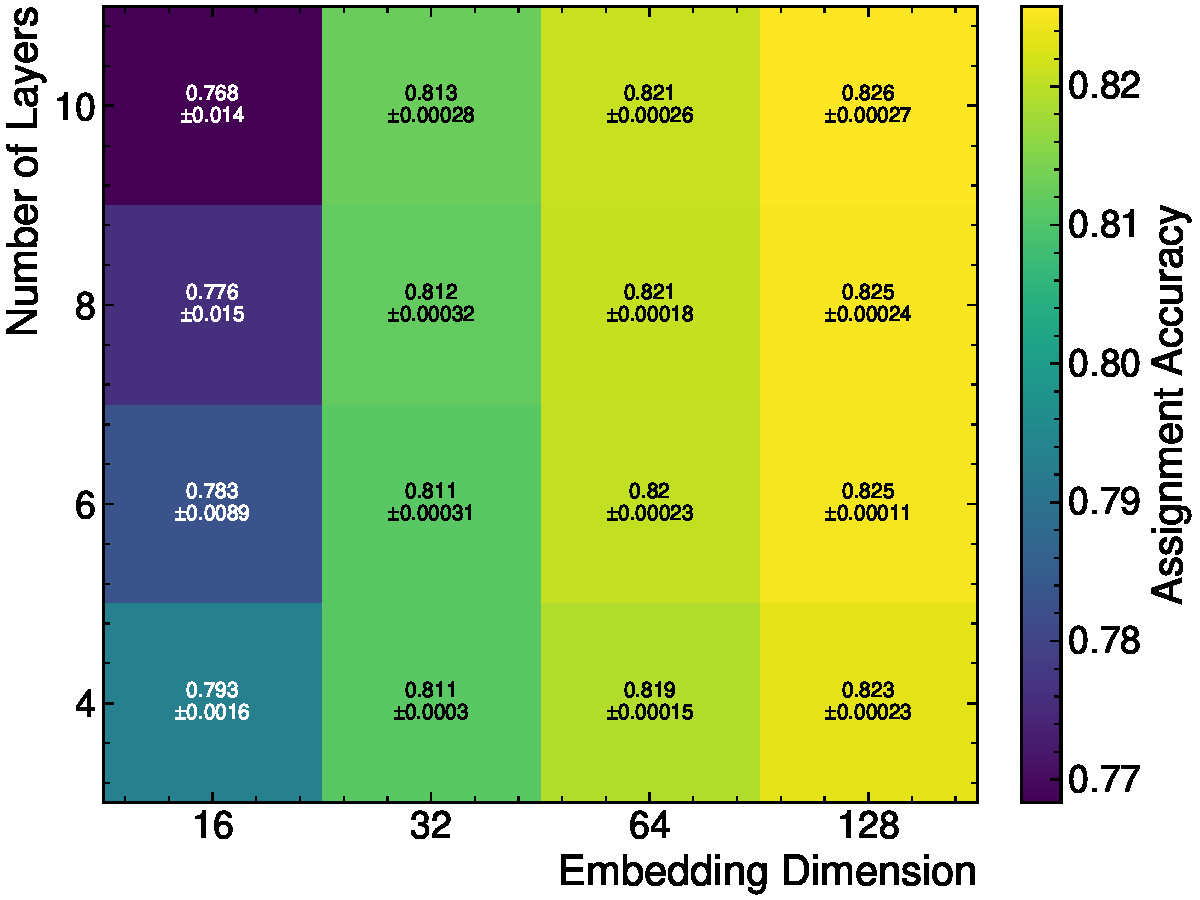
\includegraphics[width=0.7\textwidth]{plots/hyperparams_assignment/CompactTransformer_assignment_accuracy_embedding_dimension_vs_num_layers.pdf}
        \caption{Assignment Accuracy}
        \label{fig:hyperparams_compact_acc}
    \end{subfigure}
    \begin{subfigure}{1.0\textwidth}
        \centering
        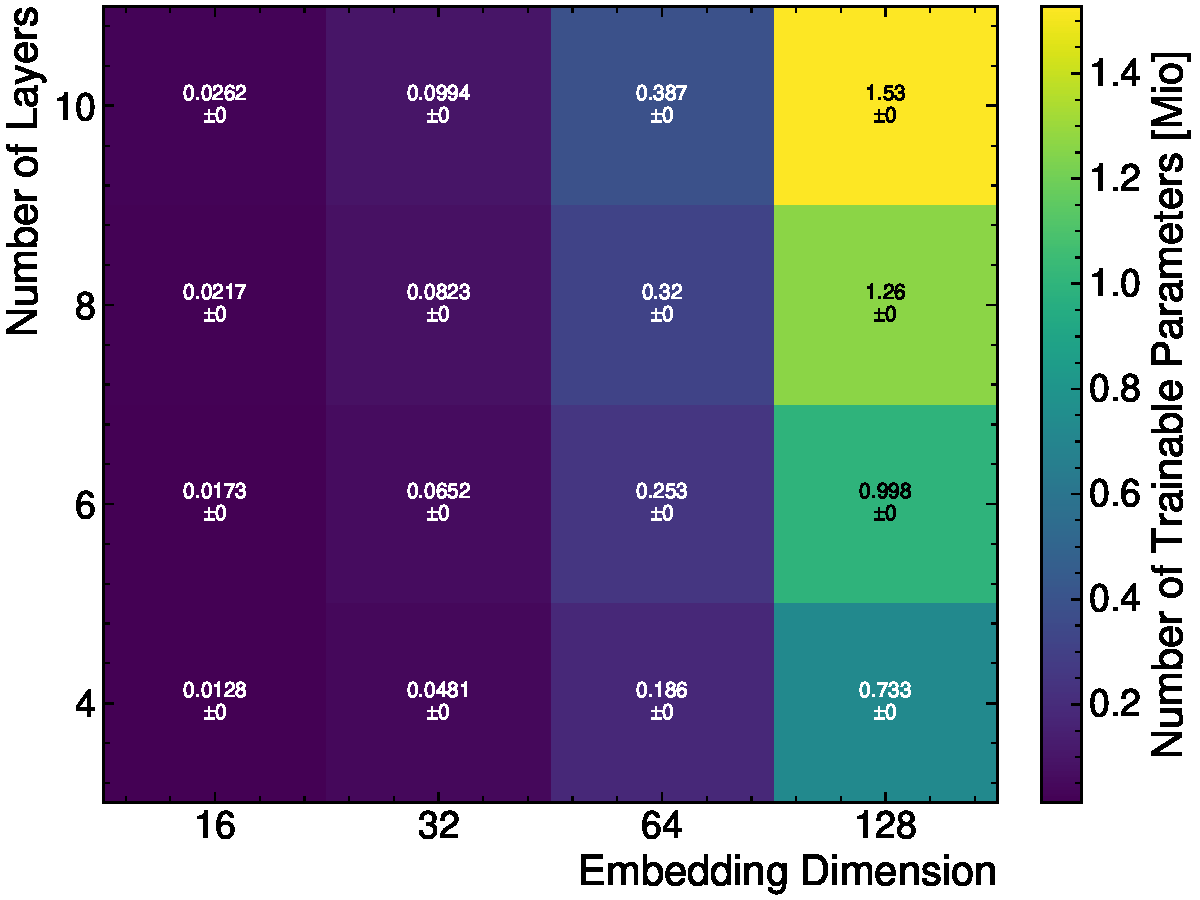
\includegraphics[width=0.7\textwidth]{plots/hyperparams_assignment/CompactTransformer_num_trainable_parameters_embedding_dimension_vs_num_layers.pdf}
        \caption{Number of Trainable Parameters}
        \label{fig:hyperparams_compact_params}
    \end{subfigure}
    \caption{The Figures \subrefb{fig:hyperparams_compact_acc} and \subrefb{fig:hyperparams_compact_params} show the assignment accuracy and the number of trainable parameters of the CompactTransformer architecture as a function of the embedding dimension and the number of transformer layers.}
    \label{fig:hyperparams_compact}
\end{figure}



\section{Performance Plots}
\subsection{Assignment Performance}
\begin{figure}[H]
    \centering
    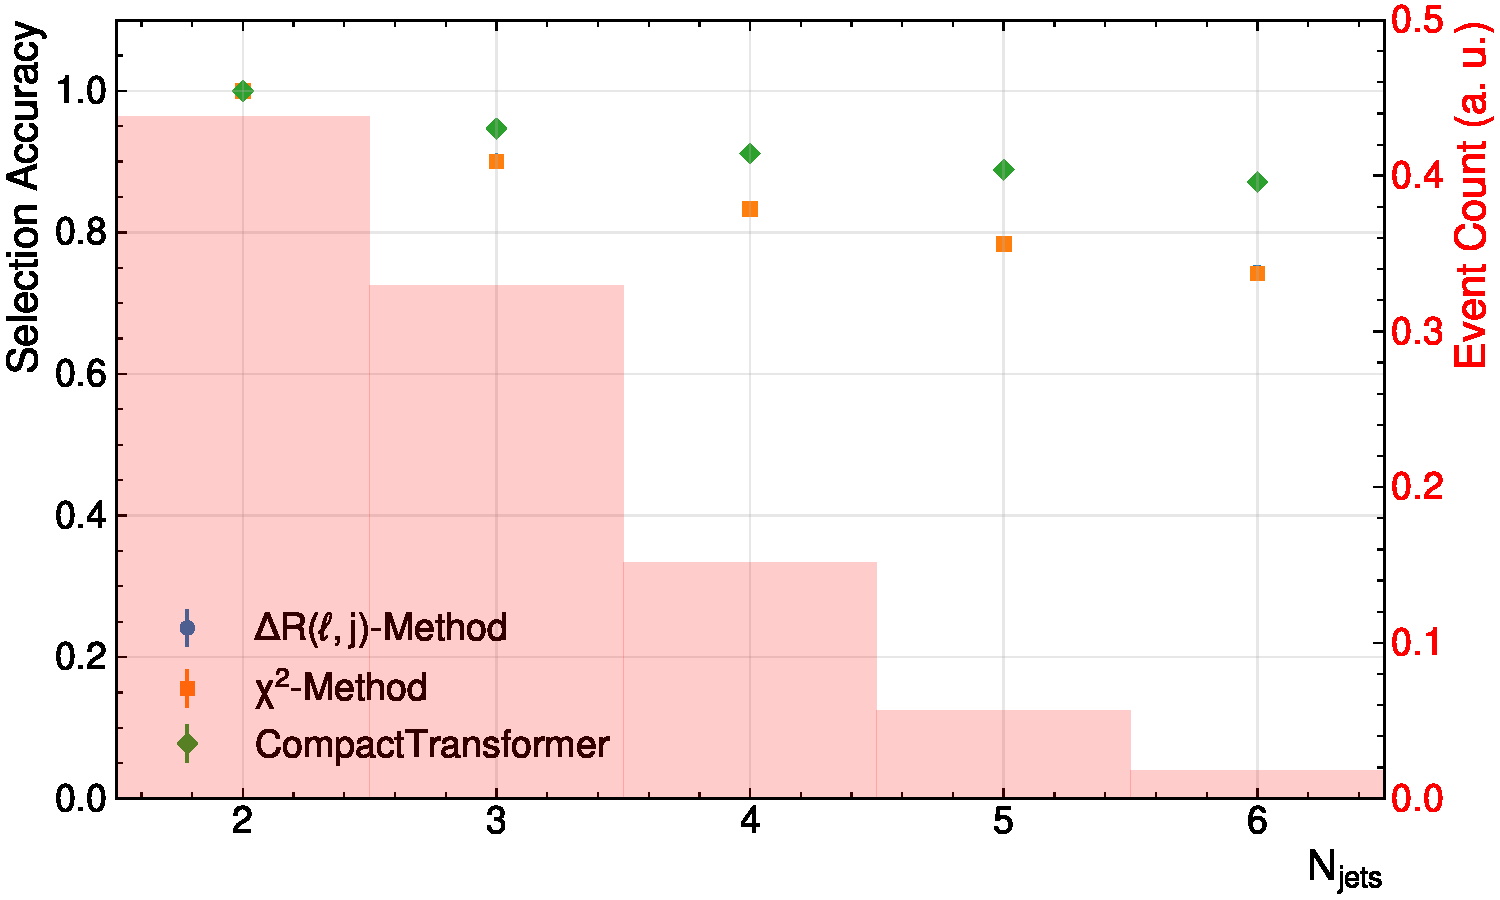
\includegraphics[width=0.7\textwidth]{plots/compact_assigner/binned_performance/N_jets/binned_selection_accuracies_N_jets.pdf}
    \caption{Selection accuracy as a function of the number of jets in the event for different reconstruction methods. The background histograms show of the distribution of events as a function of the number of jets. The uncertainties represent the statistical variations in the evaluation dataset.}
    \label{fig:selection_accuracy_vs_n_jets}
\end{figure}



\begin{figure}
    \centering
    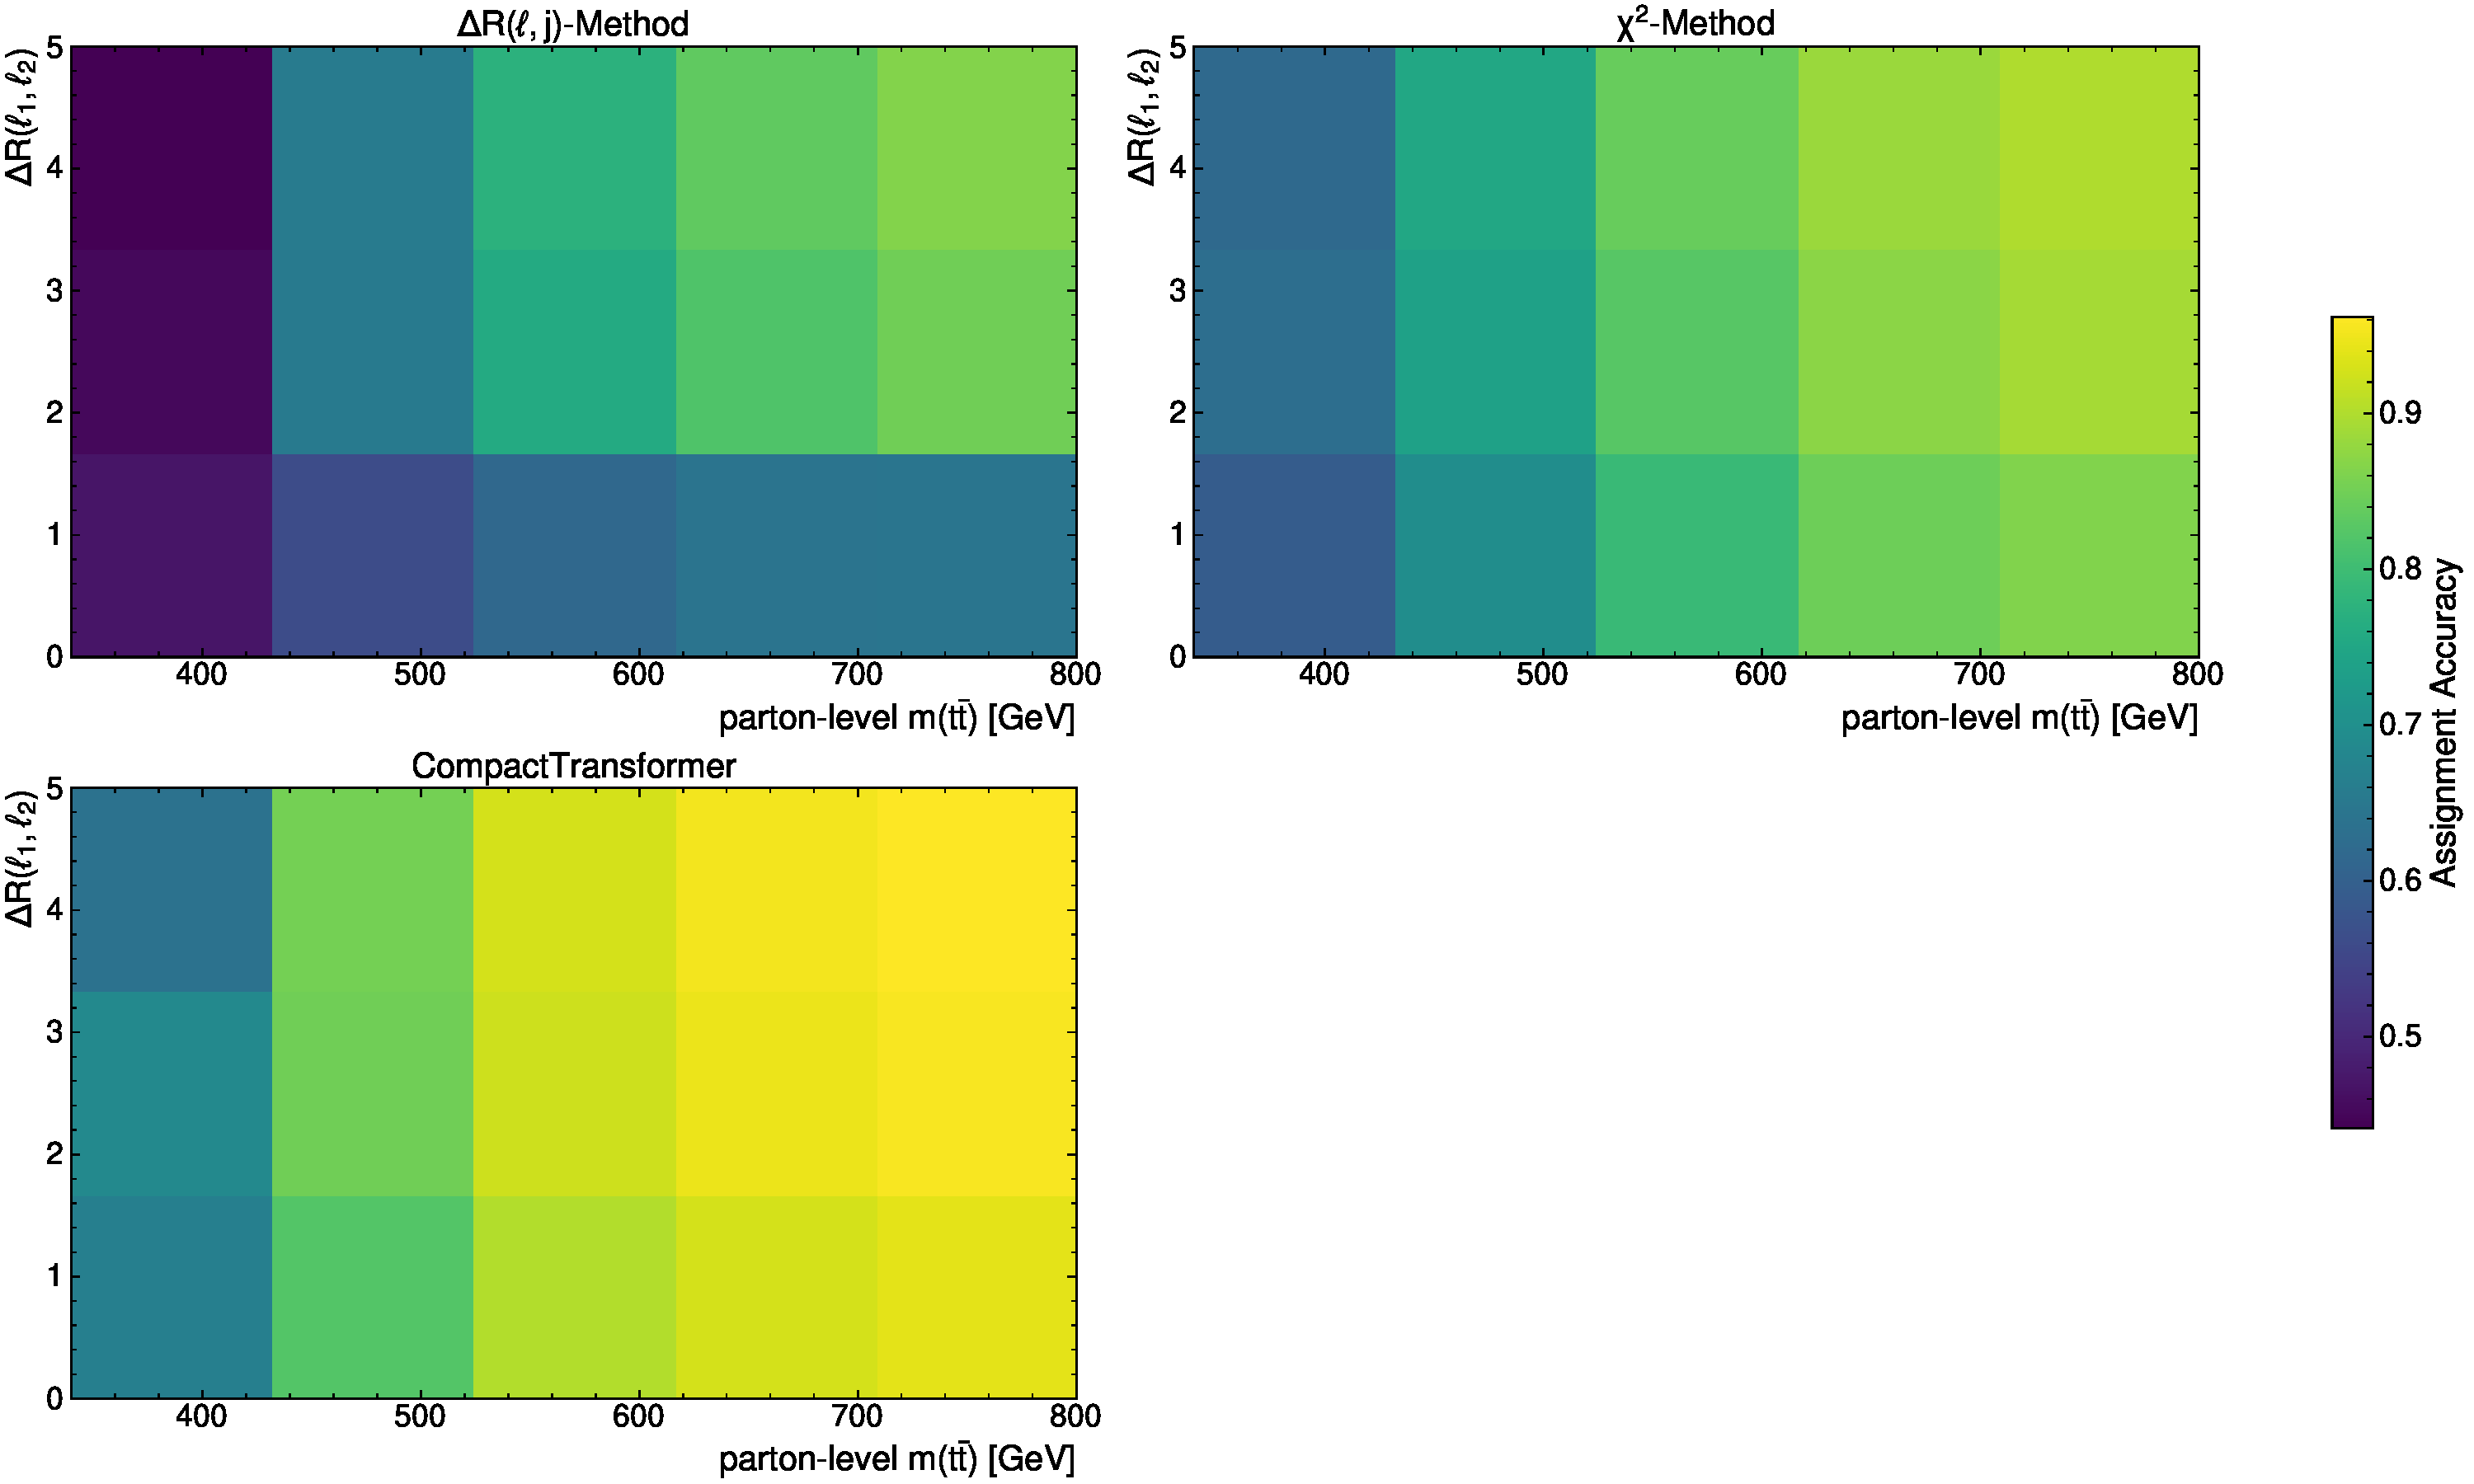
\includegraphics[width=1.0\textwidth]{plots/compact_assigner/binned_2d_performance/truth_ttbar_mass_vs_dR_l1l2/2d_binned_accuracies_truth_ttbar_mass_dR_l1l2.pdf}
    \caption{Assignment accuracy binned with respect to parton-level $m(t\bar{t})$ and $\Delta R(\ell_1,\ell_2)$.}
    \label{fig:accuracy_2d_mttbar_dR_l1l2}
\end{figure}
\chapter{Supplementary Material}
\label[appsec]{chap:supplementary_computations_and_proofs}
\section{Mathematical Foundation of Machine Learning}
\subsection{Mean Squared Error Loss and Conditional Expectation}
\label[appsec]{app:mse_mean}
When performing a minimisation of the batch loss based on the mean squared error (MSE) in a supervised learning setting, one can show that the optimal predictor corresponds to the conditional expectation of the target variable given the input features.
The MSE batch loss can be written as:
\begin{equation}
  \mathcal{L}_{\text{MSE}}(f_{\boldsymbol{\theta}}) = \frac{1}{N}
  \sum_{i=1}^{N} (\mathbf{y}_i - f_{\boldsymbol{\theta}}(\mathbf{x}_i))^2~.
\end{equation}
Using a simple calculus argument, one can show that the function $f_{\boldsymbol{\theta}}$ that minimises this batch loss is given by:
\begin{align}
  \frac{d}{d{\boldsymbol{\theta}}} \mathcal{L}_{\text{MSE}}(f_{\boldsymbol{\theta}}) & = \frac{d}{df} \int (\mathbf{y} - f_{\boldsymbol{\theta}}(\mathbf{x}))^2 p(\mathbf{y}|\mathbf{x}) \,d\mathbf{y} \cdot \frac{\partial f}{\partial {\boldsymbol{\theta}}}   \\
  & = \int 2(f_{\boldsymbol{\theta}}(\mathbf{x}) - \mathbf{y}) p(\mathbf{y}|\mathbf{x}) dy \cdot \frac{\partial   f}{\partial {\boldsymbol{\theta}}}\overset{!}{=} 0 \\
  \Rightarrow f_{\boldsymbol{\theta}}(\mathbf{x})
  & = \int \mathbf{y} p(\mathbf{y}|\mathbf{x}) \,d\mathbf{y} = \mathbb{E}_{\mathbf{y}|\mathbf{x}}(\mathbf{y})~.
\end{align}

\subsection{Equivalence of Maximum Likelihood and KL-Divergence Minimisation}
\label[appsec]{app:ml_kld}
Let $p_{\text{data}}(\mathbf{x})$ denote the true data distribution and $p_{\boldsymbol{\theta}}(\mathbf{x})$ a parametric model. The KL-divergence between them is defined as 
\begin{equation}
  D_{\text{KL}}(p_{\text{data}} \| p_{\boldsymbol{\theta}})
  = \mathbb{E}_{\mathbf{x} \sim p_{\text{data}}} \left[ \log
  \frac{p_{\text{data}}(\mathbf{x})}{p_{\boldsymbol{\theta}}(\mathbf{x})} \right]
  = \mathbb{E}_{\mathbf{x} \sim p_{\text{data}}} \left[ \log p_{\text{data}}(\mathbf{x}) \right]
  - \mathbb{E}_{\mathbf{x} \sim p_{\text{data}}} \left[ \log p_{\boldsymbol{\theta}}(\mathbf{x}) \right].
\end{equation}
Since the first term, $-H(p_{\text{data}})$, is the negative entropy of the data distribution and does not depend on ${\boldsymbol{\theta}}$, minimising the KL-divergence over ${\boldsymbol{\theta}}$ is equivalent to \begin{equation}
  \hat{{\boldsymbol{\theta}}} = \argmin_{\boldsymbol{\theta}} D_{\text{KL}}(p_{\text{data}} \| p_{\boldsymbol{\theta}})
  = \argmax_{\boldsymbol{\theta}} \, \mathbb{E}_{\mathbf{x} \sim p_{\text{data}}} \left[ \log
  p_{\boldsymbol{\theta}}(\mathbf{x}) \right].
\end{equation}
Approximating the expectation over $p_{\text{data}}$ by the empirical mean over a dataset $\{x_i\}_{i=1}^{N}$ of $N$ independent observations gives \begin{equation}
  \hat{{\boldsymbol{\theta}}} = \argmax_{\boldsymbol{\theta}} \frac{1}{N} \sum_{i=1}^{N} \log
  p_{\boldsymbol{\theta}}(\mathbf{x}_i),=\argmin_{\boldsymbol{\theta}} \frac{1}{N} \sum_{i=1}^{N} -\log p_{\boldsymbol{\theta}}(\mathbf{x}_i)
\end{equation}
which is precisely the maximum likelihood estimator. Note that this simply generalises to the case of a conditional probability.

\subsection{Gaussian-Loss as Minimisation of the KL-divergence}
\label[appsec]{app:gaussian_loss}
Assume the conditional parametric model to have the form of a (multidimensional) Gaussian distribution,
\begin{equation}
  p_{\boldsymbol{\theta}}(\mathbf{y}|\mathbf{x})=\prod_i^{\text{dim}}\frac{1}{\sqrt{2\pi\sigma_{i,{\boldsymbol{\theta}}}^2(\mathbf{x})}}\exp\left(-\frac{(y_i-\mu_{i,{\boldsymbol{\theta}}}^2(\mathbf{x}))^2}{2\sigma_{i,{\boldsymbol{\theta}}}^2(\mathbf{x})}\right)~.
\end{equation}
For this, one can now consider the negative log-likelihood (NLL) of a dataset of $\{x_j\}_{j=1}^{N}$ of $N$ independent observations:
\begin{align}
  \text{NLL}(p_{\boldsymbol{\theta}})&=\frac{1}{N}\sum_{j=1}^N-\log(p_{\boldsymbol{\theta}}(\mathbf{y}|\mathbf{x}))\\
  &=\frac{1}{N}\sum_{j=1}^N\sum_{i=1}^{\text{dim}}\left(\frac{1}{2}\log(2\pi)+\frac{1}{2}\log(\sigma_{i,{\boldsymbol{\theta}}}^2(\mathbf{x}))+\frac{(y_i-\mu_{i,{\boldsymbol{\theta}}}^2(\mathbf{x}))^2}{2\sigma_{i,{\boldsymbol{\theta}}}^2(\mathbf{x})}\right)~.
\end{align}
The constant term $\log(2\pi)$ can be dropped for the minimisation, which results in \begin{align}
  \hat{\boldsymbol{\theta}}&=\argmin_{\boldsymbol{\theta}} \text{NLL}(p_{\boldsymbol{\theta}})\\
  &=\argmin_{\boldsymbol{\theta}} \frac{1}{N}\sum_{j=1}^N\sum_{i=1}^\text{dim}\left(2\log(\sigma_{i,{\boldsymbol{\theta}}}(\mathbf{x}))+\frac{(y_i-\mu_{i,{\boldsymbol{\theta}}}^2(\mathbf{x}))^2}{\sigma_{i,{\boldsymbol{\theta}}}^2(\mathbf{x})}\right)~.
\end{align}

\section{Neutrino Momenta Posterior Distributions}
\label[appsec]{app:neutrino_probs}
\subsection{Invariant Mass of Top-Quark Pair}
\begin{figure}[H]
  \centering
  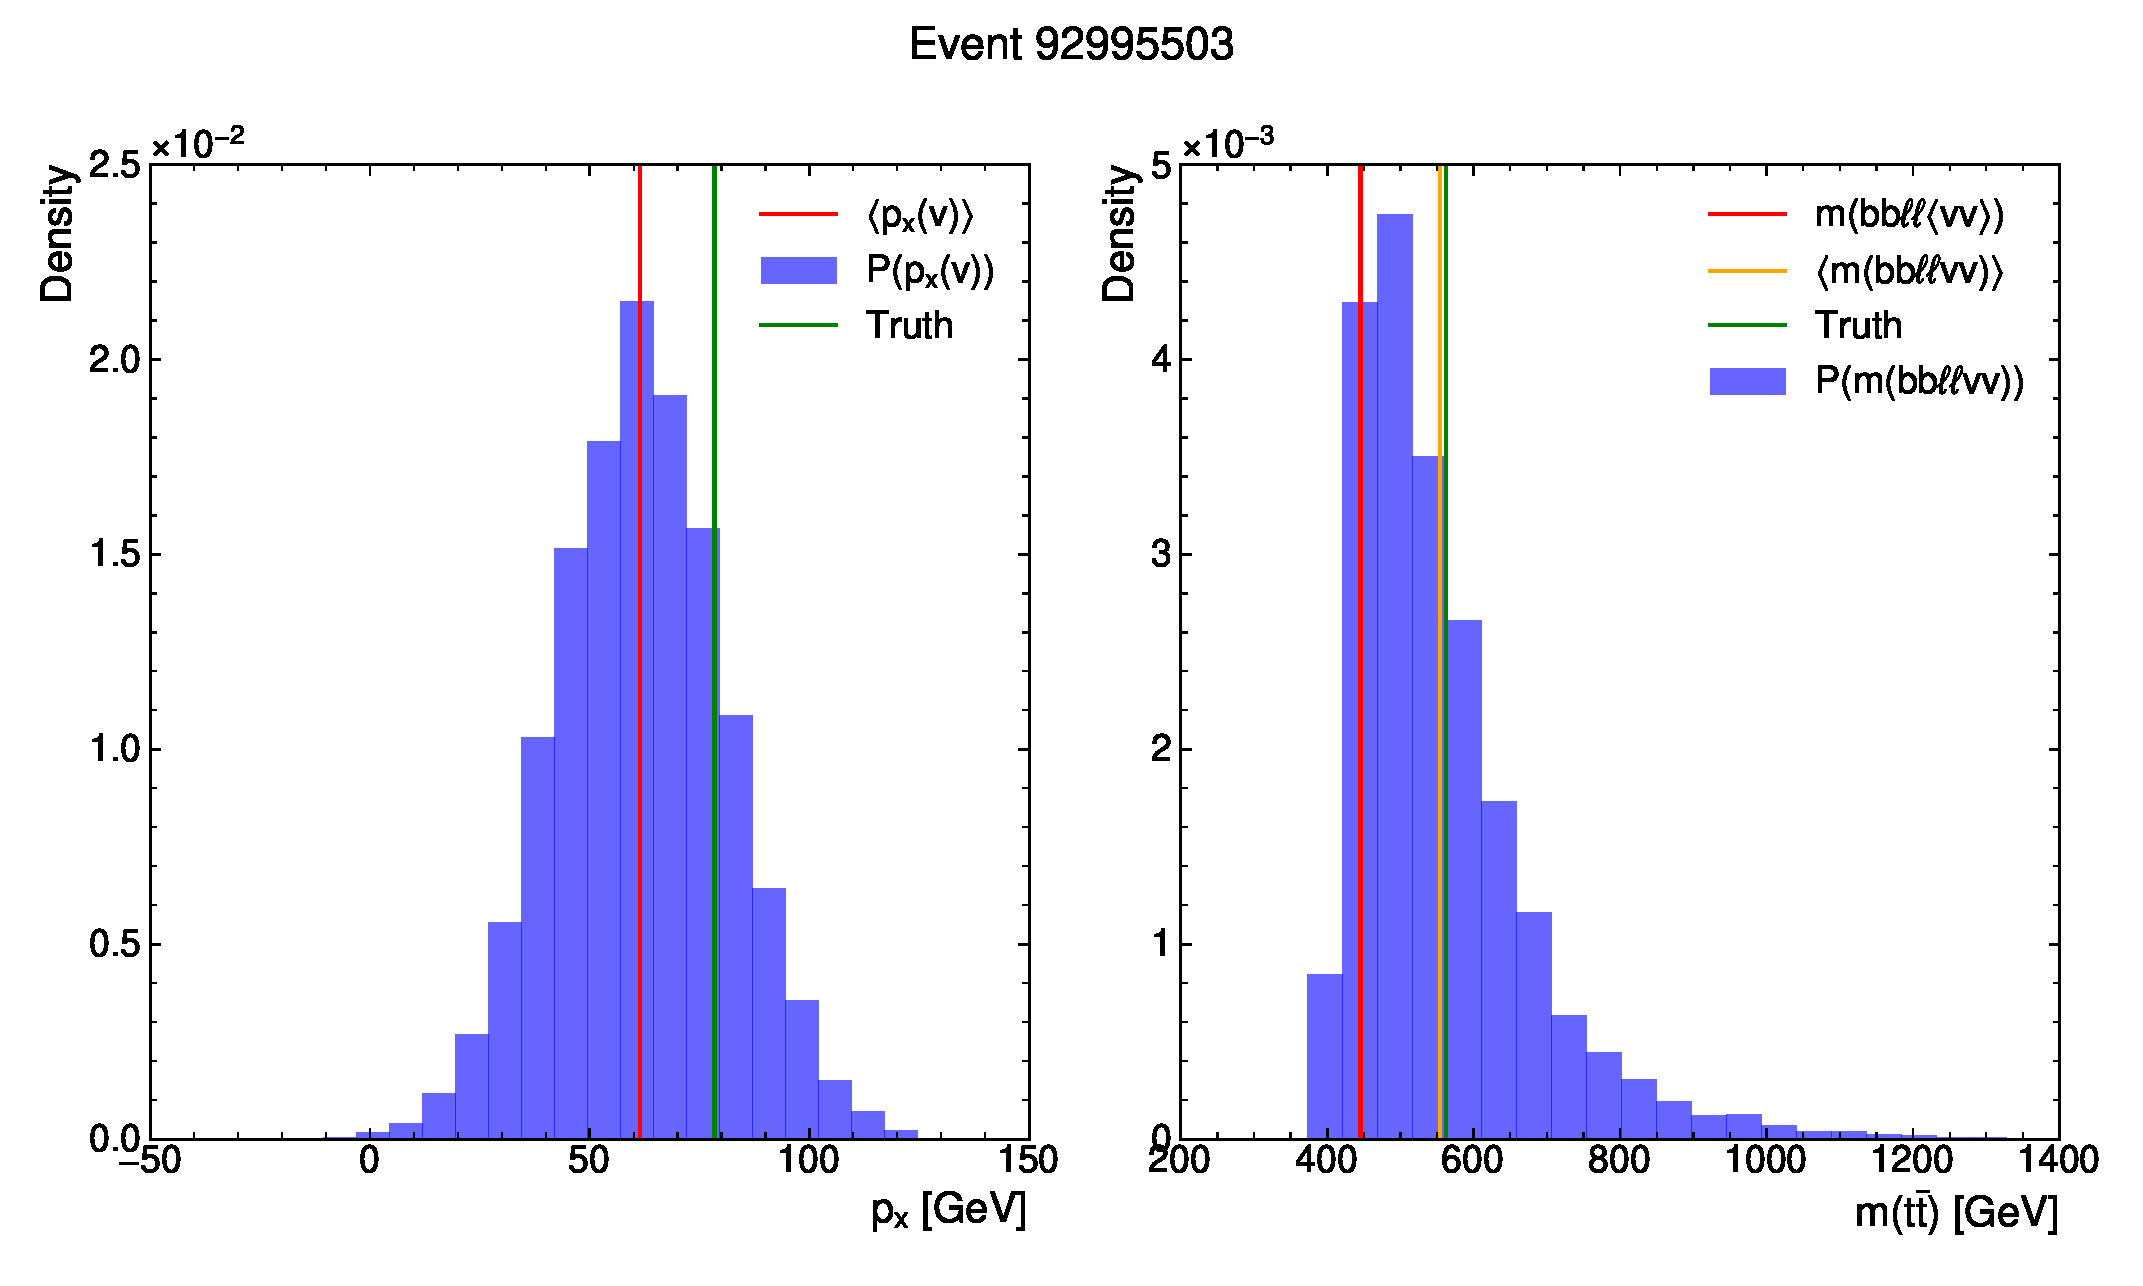
\includegraphics[width=1.0\textwidth]{plots/gaussian_loss_plots/gaussian_loss_sample_mttbar_plots.pdf}
  \caption{Plots showing the probability distribution of the neutrino momentum component $p_x$ and the reconstructed invariant mass $m(t\bar{t})$ based on the mean and standard deviation predicted by the MMT-model trained with a Gaussian-loss for a random event.}
  \label{fig:gaussian_loss:mttbar_posterior_sample}
\end{figure}


\subsection{Spin-Sensitive Variable \chel}
\begin{figure}[H]
  \centering
  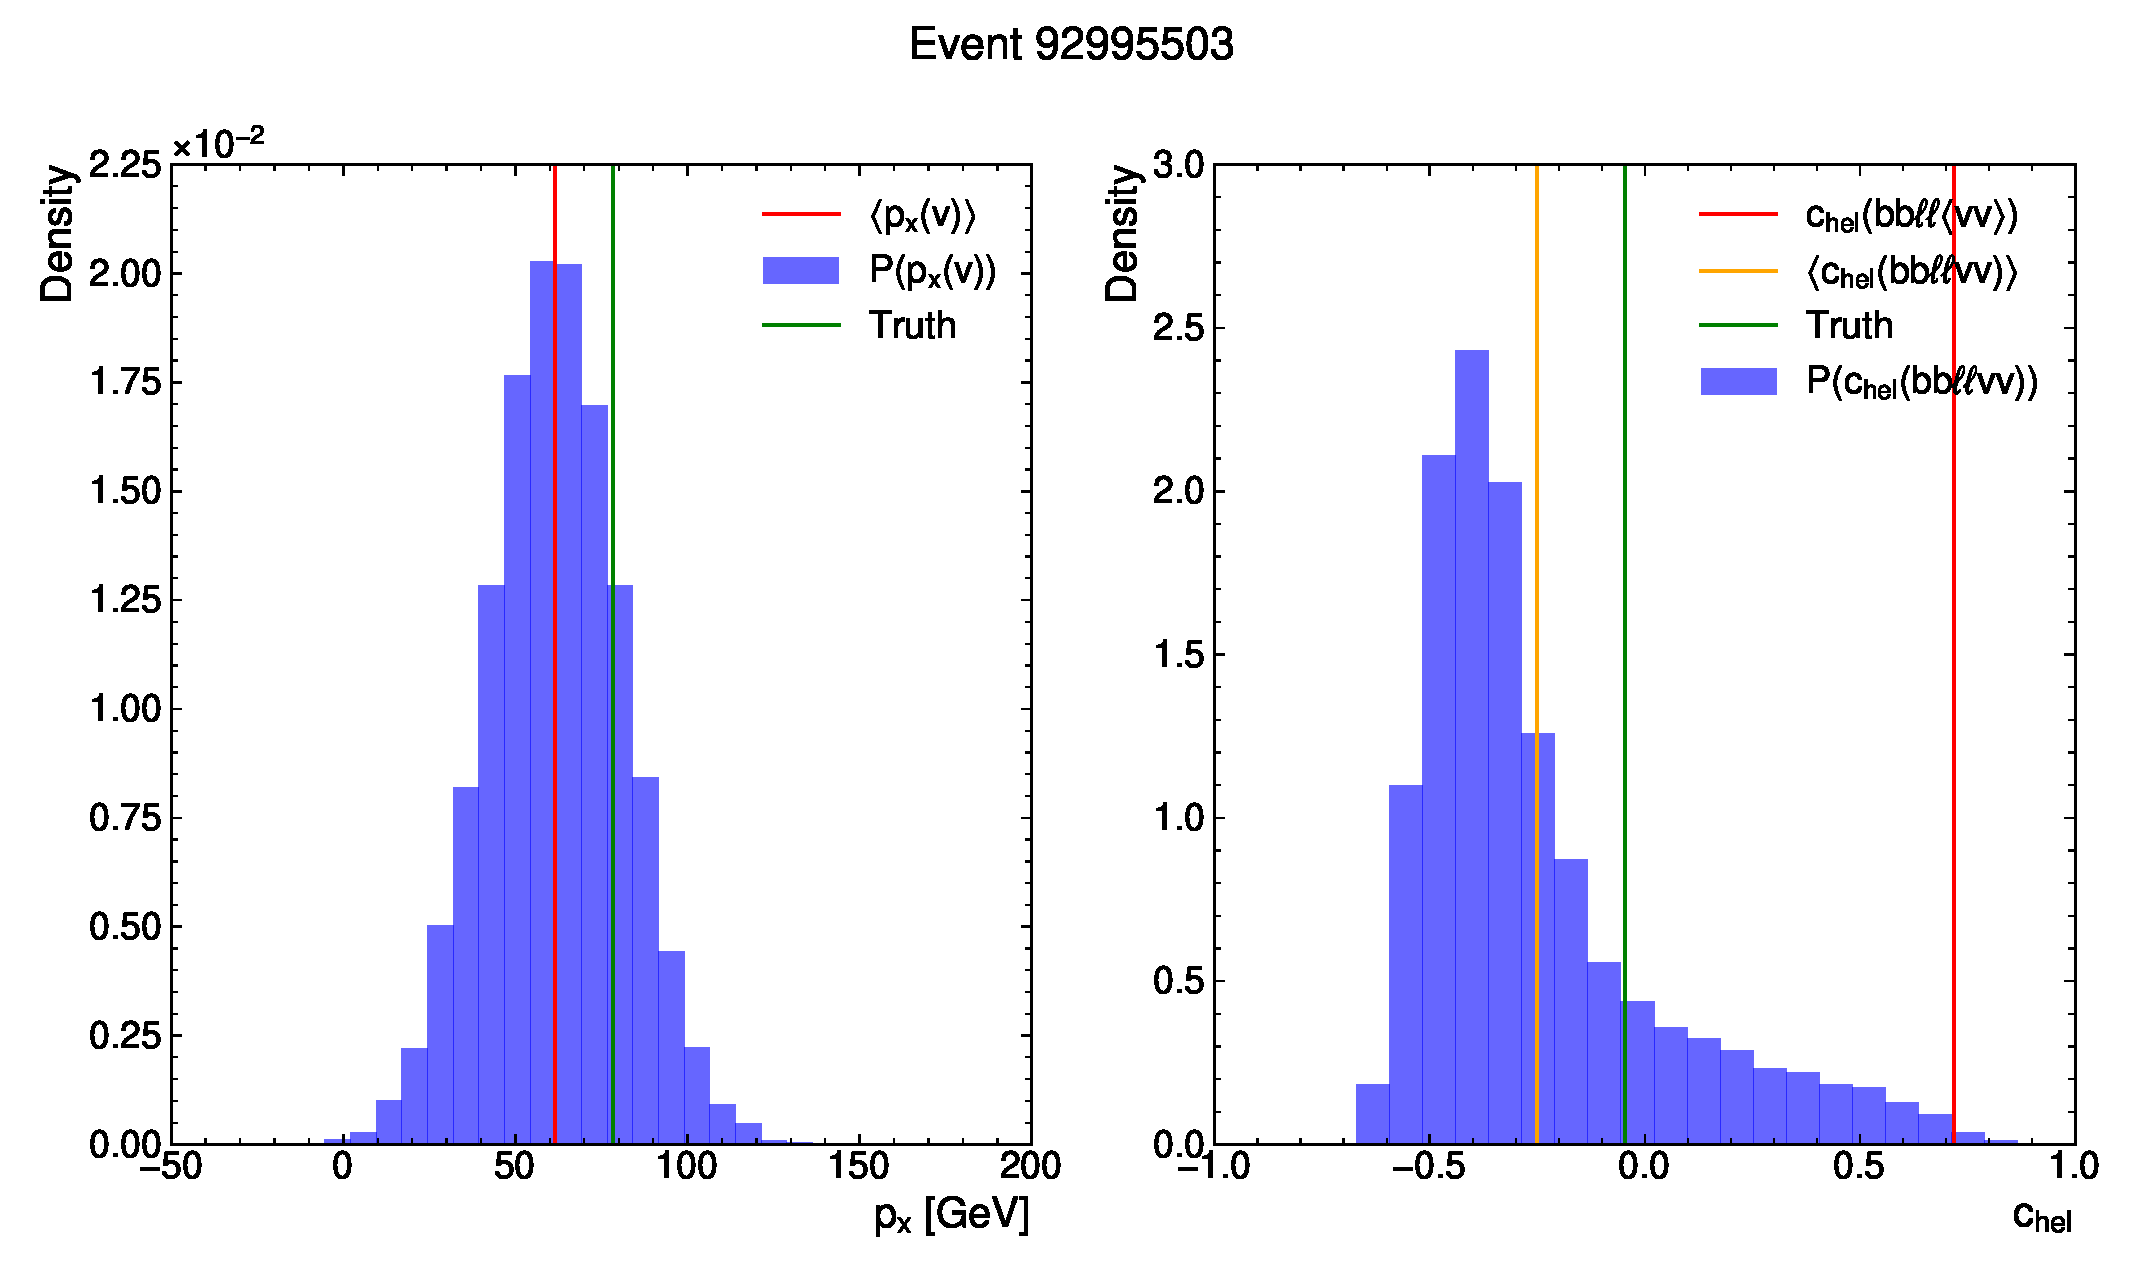
\includegraphics[width=1.0\textwidth]{plots/gaussian_loss_plots/gaussian_loss_sample_c_hel_plots.pdf}
  \caption{Plots showing the probability distribution of the neutrino momentum component $p_x$ and the reconstructed \chel based on the mean and standard deviation predicted by the MMT-model trained with a Gaussian-loss for a random event. Indicated are the mean and true values by vertical lines.}
  \label{fig:gaussian_loss:c_hel_posterior_sample}
\end{figure}
\begin{figure}[H]
  \centering
  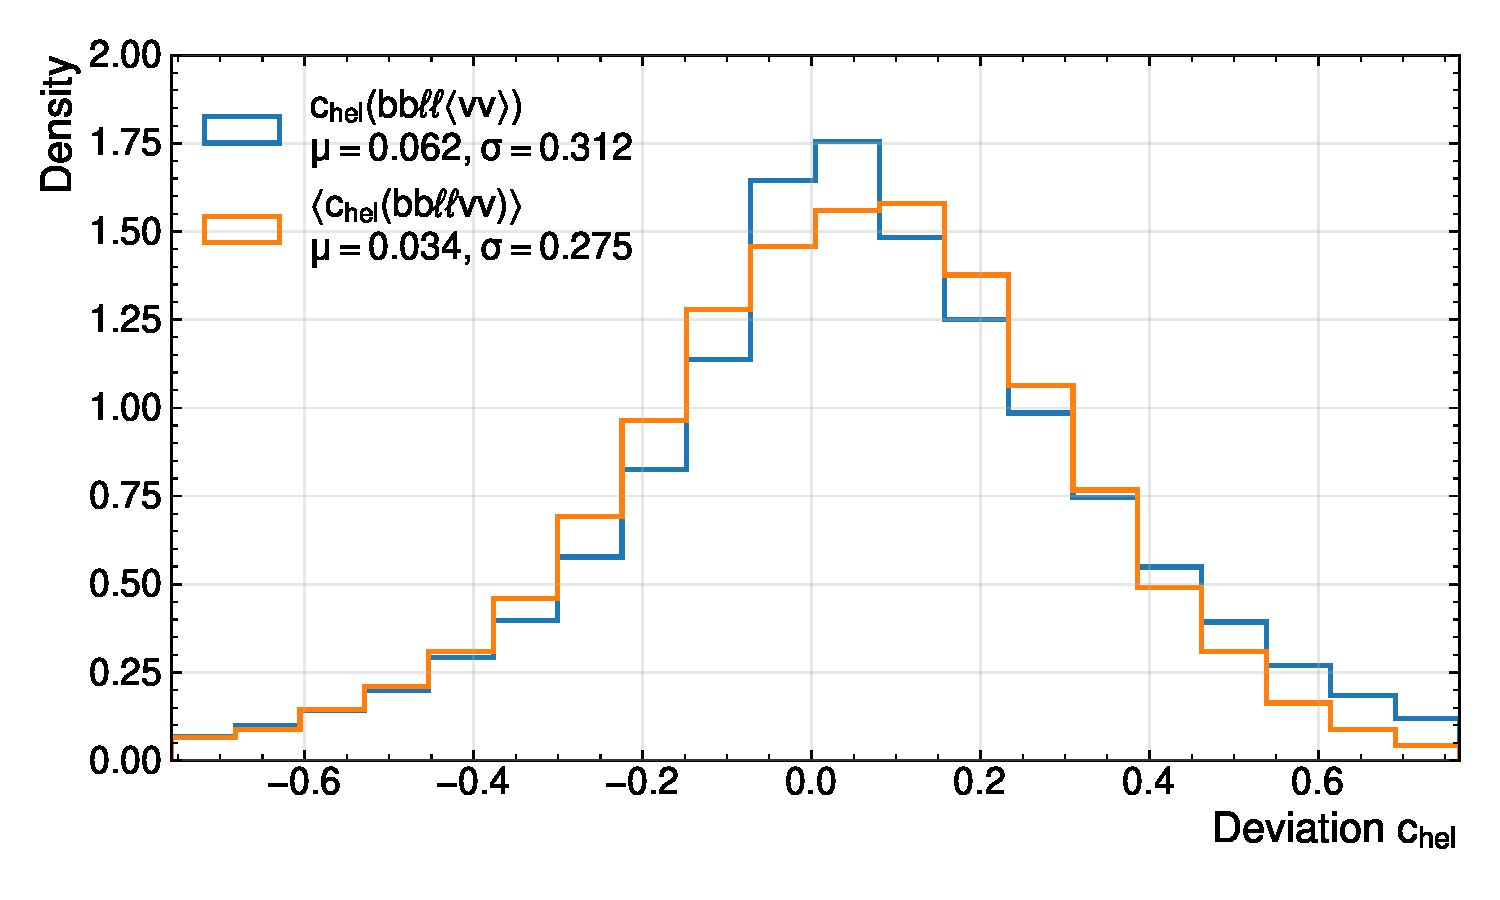
\includegraphics[width=0.7\textwidth]{plots/gaussian_loss_plots/gaussian_loss_c_hel_posterior_deviation.pdf}
  \caption{Deviation between the reconstructed and true \chel. The different curves show, whether the invariant mass was computed using the mean momentum or by propagating the neutrino probabilities and averaging of the obtained spin-variable.}
  \label{fig:gaussian_loss:c_hel_posterior_deviation}
\end{figure}

\subsection{Spin-Sensitive Variable \chan}
\begin{figure}[H]
  \centering
  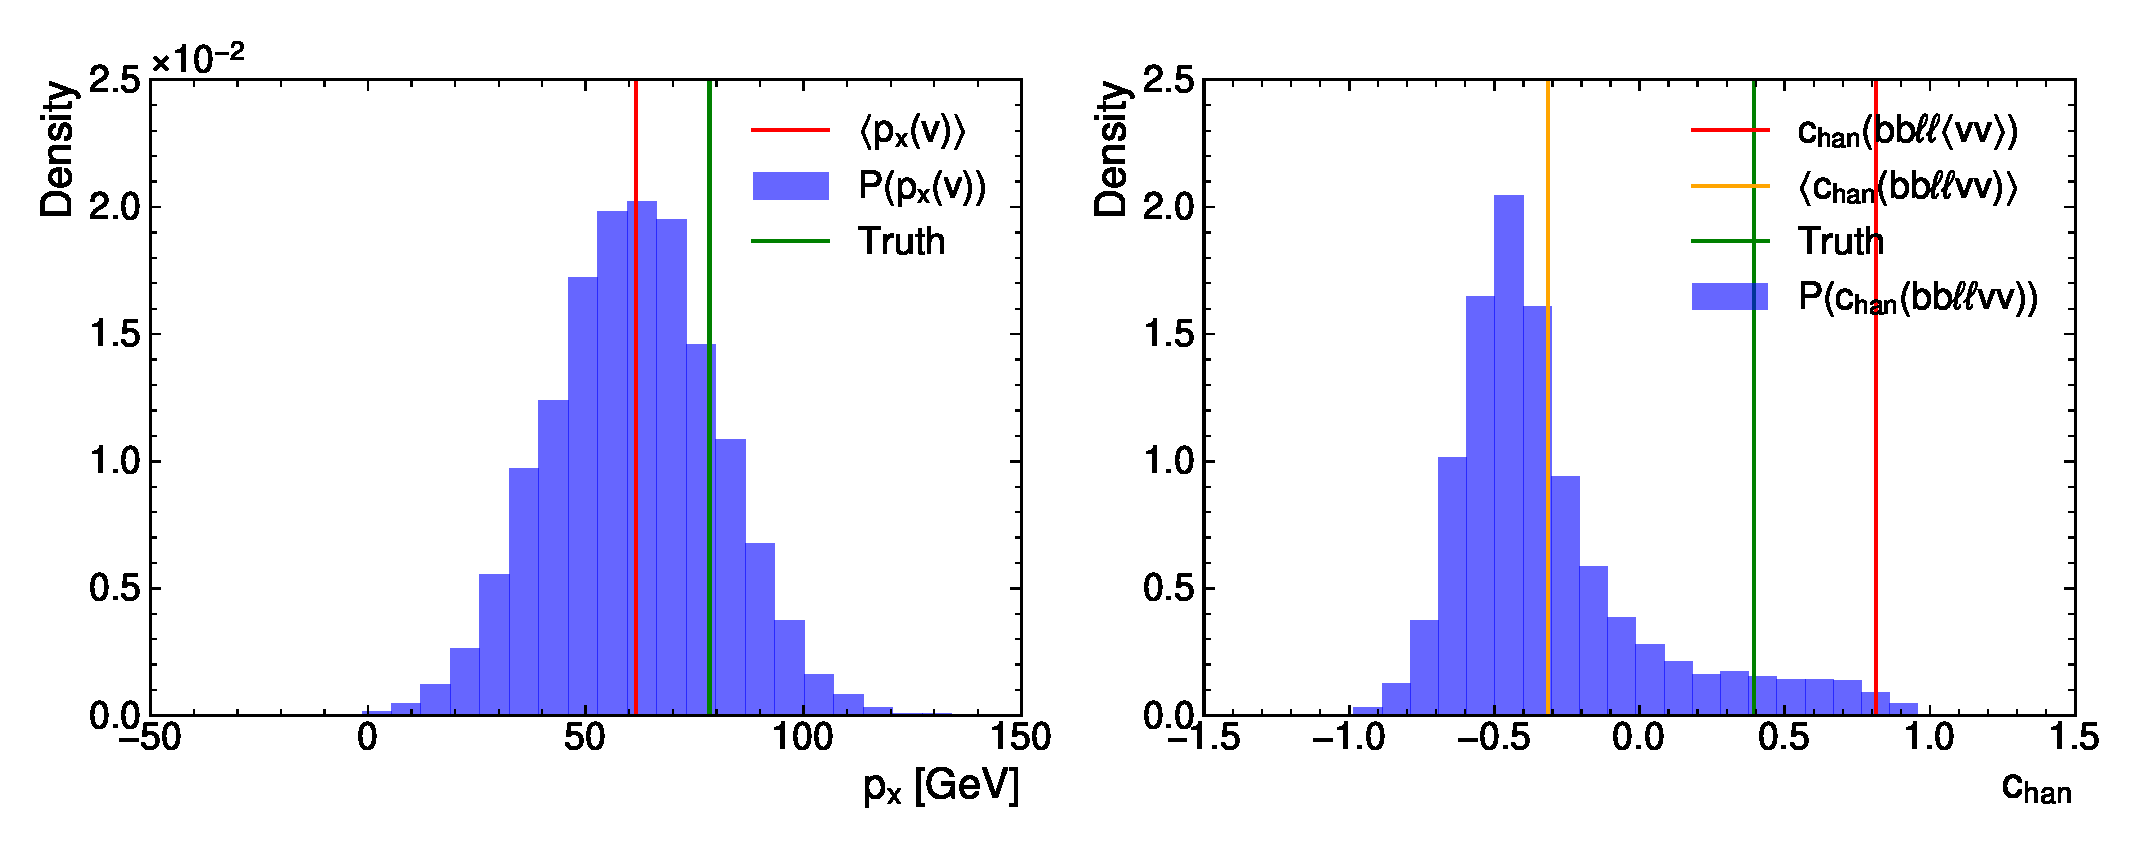
\includegraphics[width=1.0\textwidth]{plots/gaussian_loss_plots/gaussian_loss_sample_c_han_plots.pdf}
  \caption{Plots showing the probability distribution of the neutrino momentum component $p_x$ and the reconstructed \chan based on the mean and standard deviation predicted by the MMT-model trained with a Gaussian-loss for a random event. Indicated are the mean and true values by vertical lines.}
  \label{fig:gaussian_loss:c_han_posterior_sample}
\end{figure}
\begin{figure}[H]
  \centering
  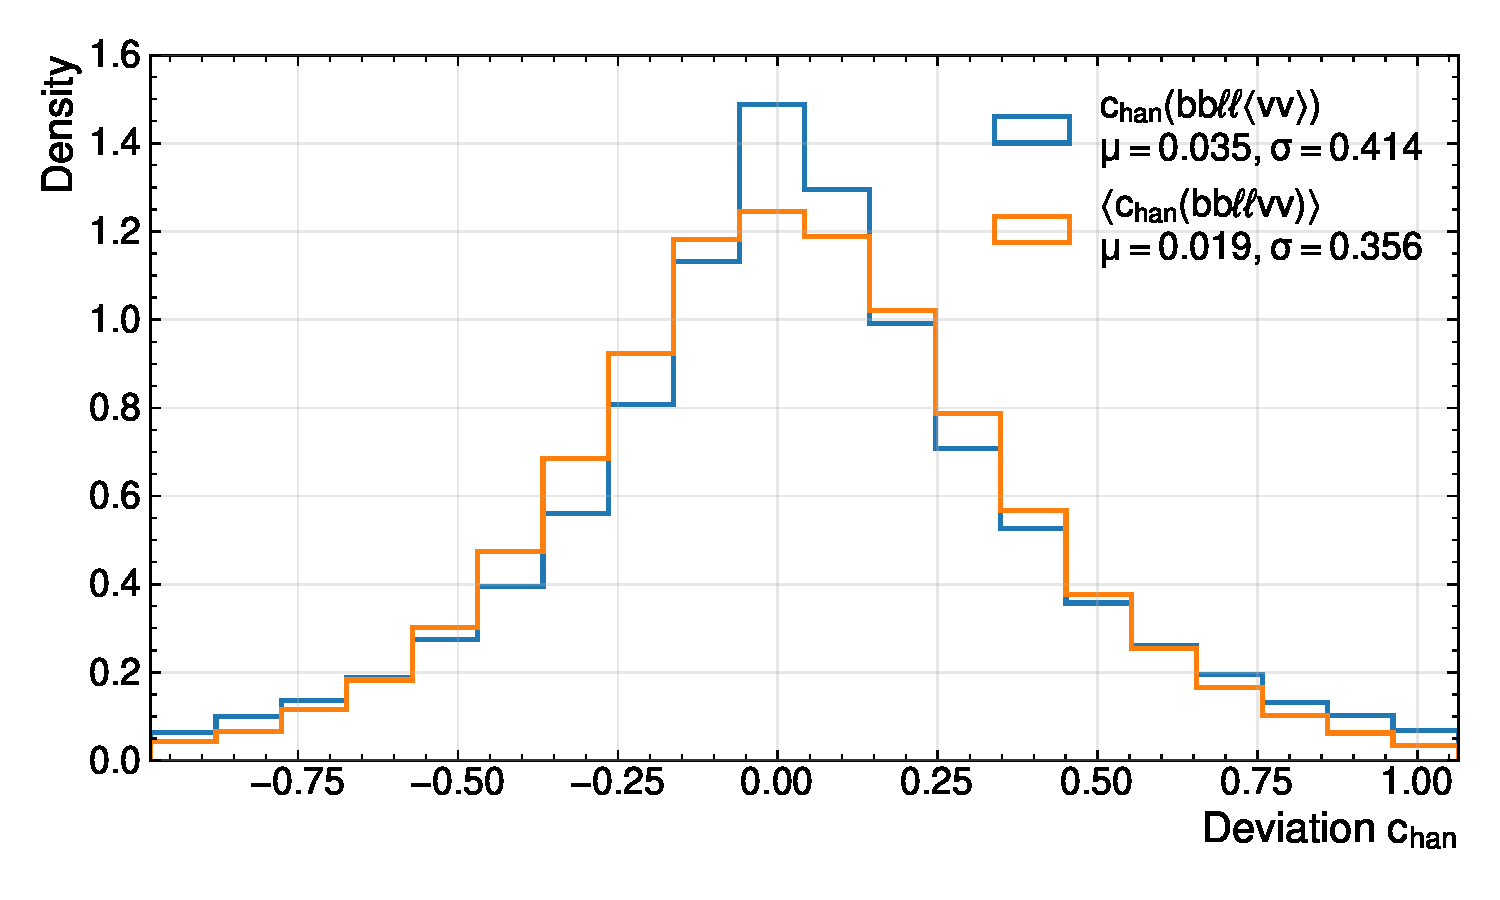
\includegraphics[width=0.7\textwidth]{plots/gaussian_loss_plots/gaussian_loss_c_han_posterior_deviation.pdf}
  \caption{Deviation between the reconstructed and true \chan. The different curves show, whether the invariant mass was computed using the mean momentum or by propagating the neutrino probabilities and averaging of the obtained spin-variable.}
  \label{fig:gaussian_loss:c_han_posterior_deviation}
\end{figure}


\cleardoublepage

\bibliography{bthesis_datenbank}

\chapter*{Acknowledgements}
There are numerous people, that have supported me along my path, mentioning all of them here would certainly exceed the scope of this thesis. However, I still want to try to give credit to the people that made this entire thesis possible.

First and foremost, I would like to express my deepest gratitude to Dr. Katharina Behr. She took me on as a student and provided me with the opportunity to work on this topic. Her guidance, support, and encouragement have been invaluable throughout this journey. She always supported me in pursuing my ideas and provided me with the freedom to explore different approaches, which has been crucial for the development of this thesis. She also enabled me to present my work at conferences and workshops, which has been an invaluable experience for me. I am truly grateful for her mentorship and the
opportunities she has given me.

Next, I want to thank Prof. Dr. Stan Lai. Despite me not being engaged in his research, he took on the supervision of this thesis. He also guided me through the administrative jungle to finish this degree and helped me with applications for PhD-positions. Taking on all of this extra work, despite me not being part of your core research group, is incredibly kind and deserves admiration.

Furthermore, I want to express my thanks to all members of Dr. Behr's
research group at DESY: Eleanor, Fiona, Lucas, and Constant.

\begin{otherlanguage}{ngerman}
  \Declaration
\end{otherlanguage}
\end{document}
